\chapter{モジュール設計}
\section{前提}
我々は\texttt{Ruby on rails}を用いて開発を行う.この言語の慣習にのっとり,これ以降,
\begin{itemize}
    \item index
    \item new
    \item show
    \item edit
    \item create
    \item destroy
    \item update
    \item home
\end{itemize}
の8つは「アクション」と呼び,これ以外の関数をすべて「メソッド」と呼ぶ.\par
アクションはコントローラが異なれば同名のものを使用するため,モジュールIDを「コントローラ名.アクション名」
とする.また,1アクション1機能を持つ.

\section{モジュール詳細}
以下に,各モジュールについて「定義書」「フロー図」の順で示す.

\clearpage

%index
\subsection*{UsersController クラスの index アクション}
ユーザを一覧する機能を持つ.対応するviewファイルを描画する.
\begin{figure}[H]
    \centering
    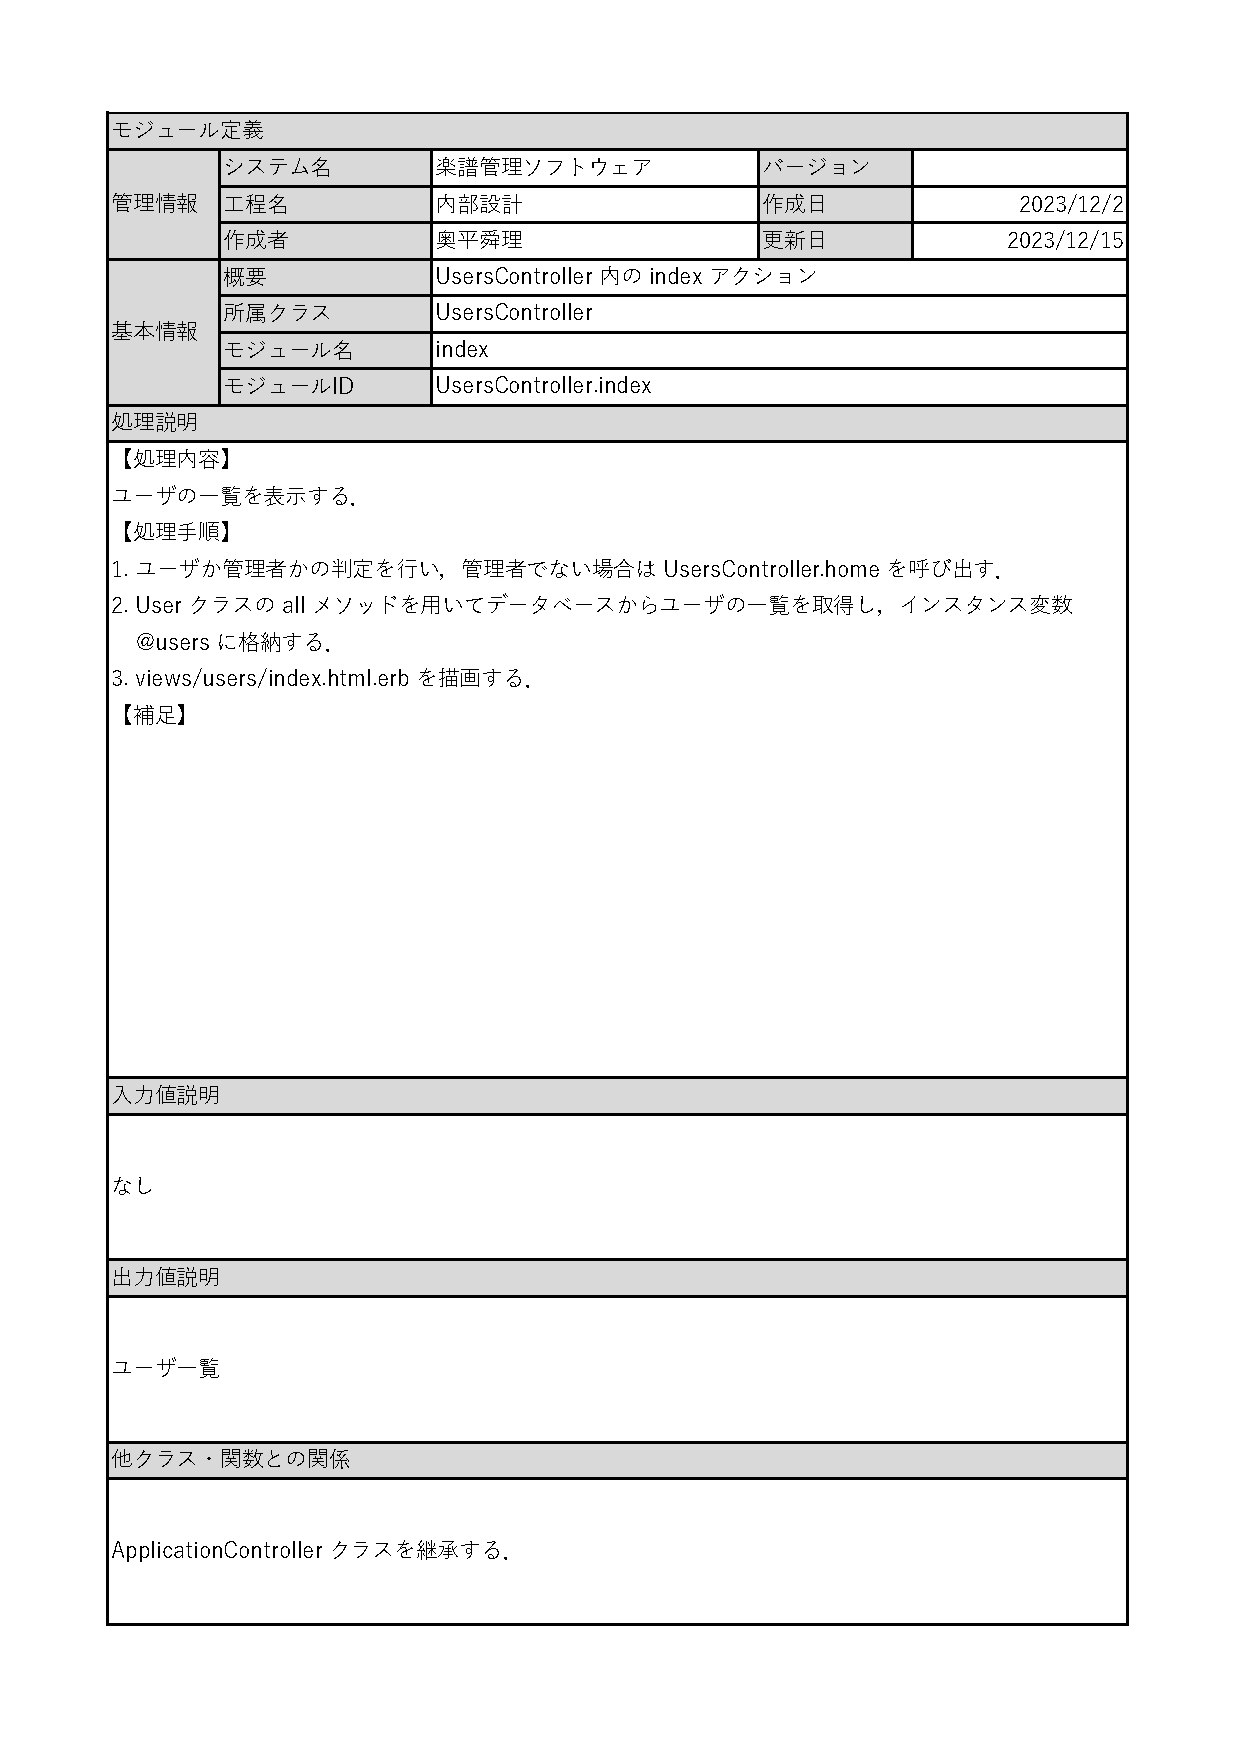
\includegraphics[scale=0.6]{img/Users/xlsx/UsersController_index.pdf}
    \vspace{-1cm}
    \caption{UsersController.index定義書}
\end{figure}
\begin{figure}
    \centering
    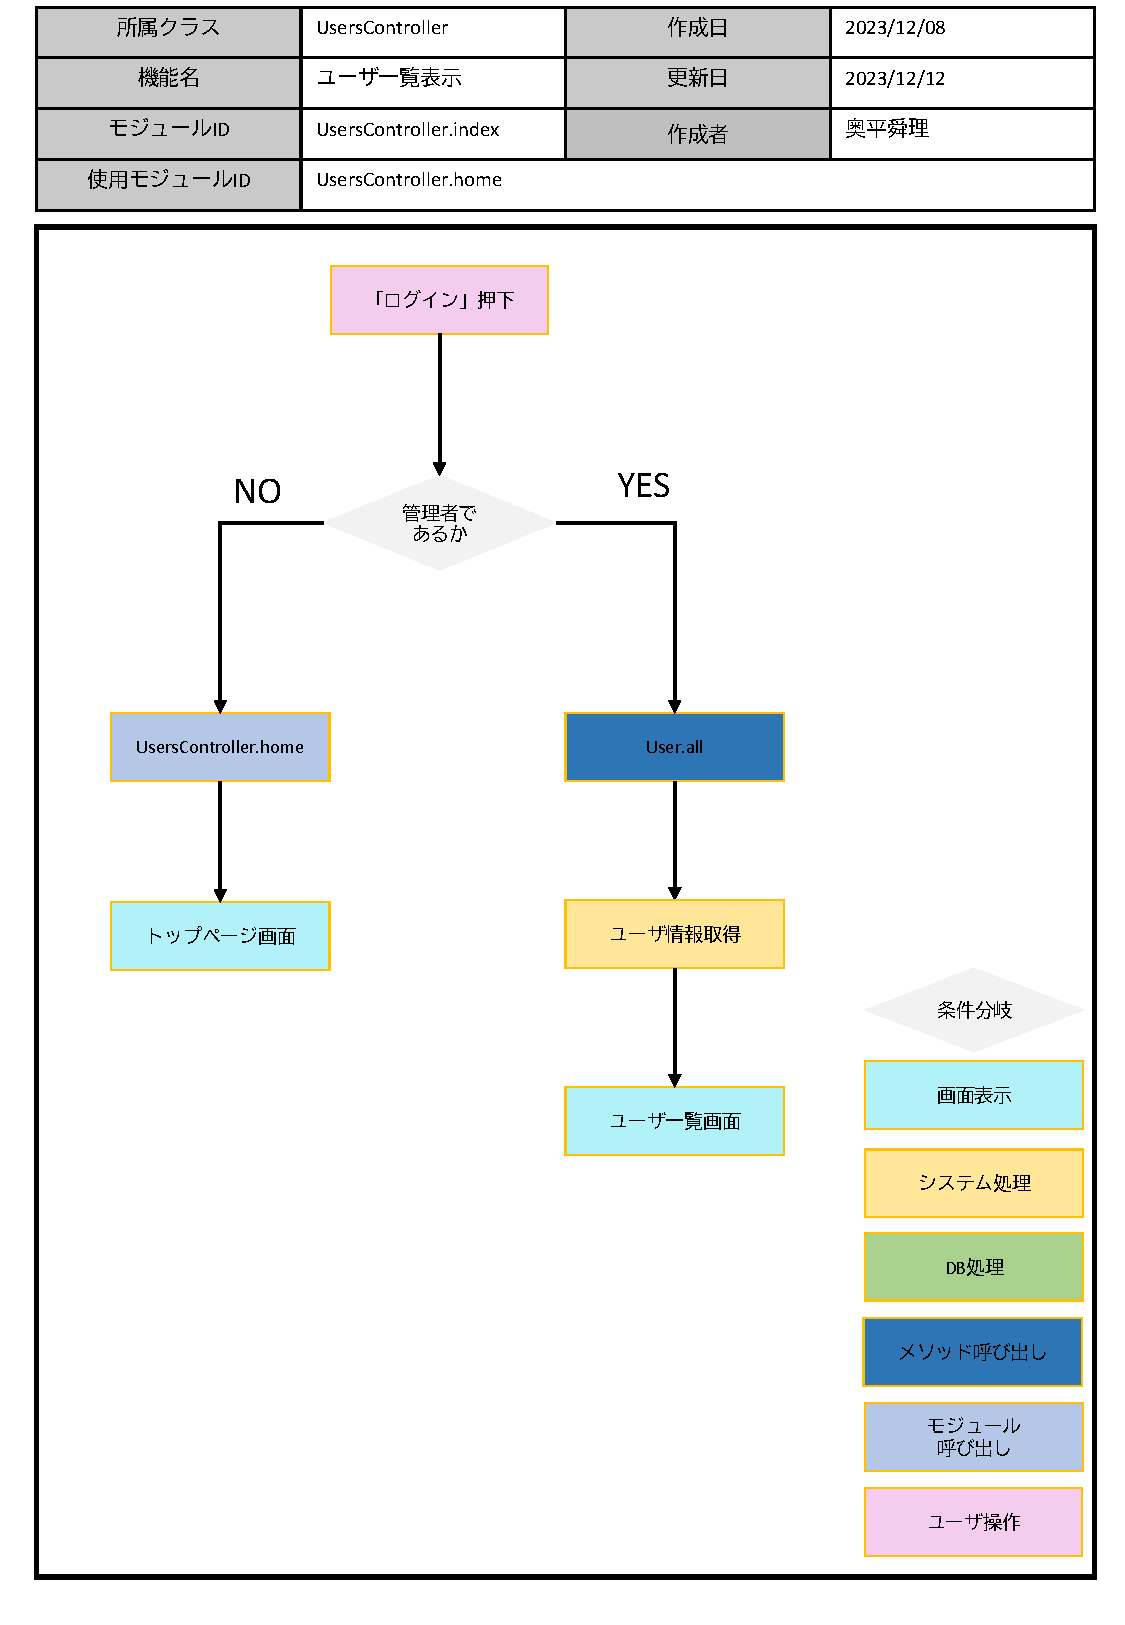
\includegraphics[scale=0.6]{img/Users/pptx/UsersController_index.pdf}
    \caption{UsersController.indexフロー図}
\end{figure}
\clearpage
\subsection*{UsersController クラスの home アクション}
楽譜データの一覧を表示するモジュール.ユーザに紐づいた楽譜データを一覧する機能を持つ.
対応するviewファイルを描画する.
\begin{figure}[H]
    \centering
    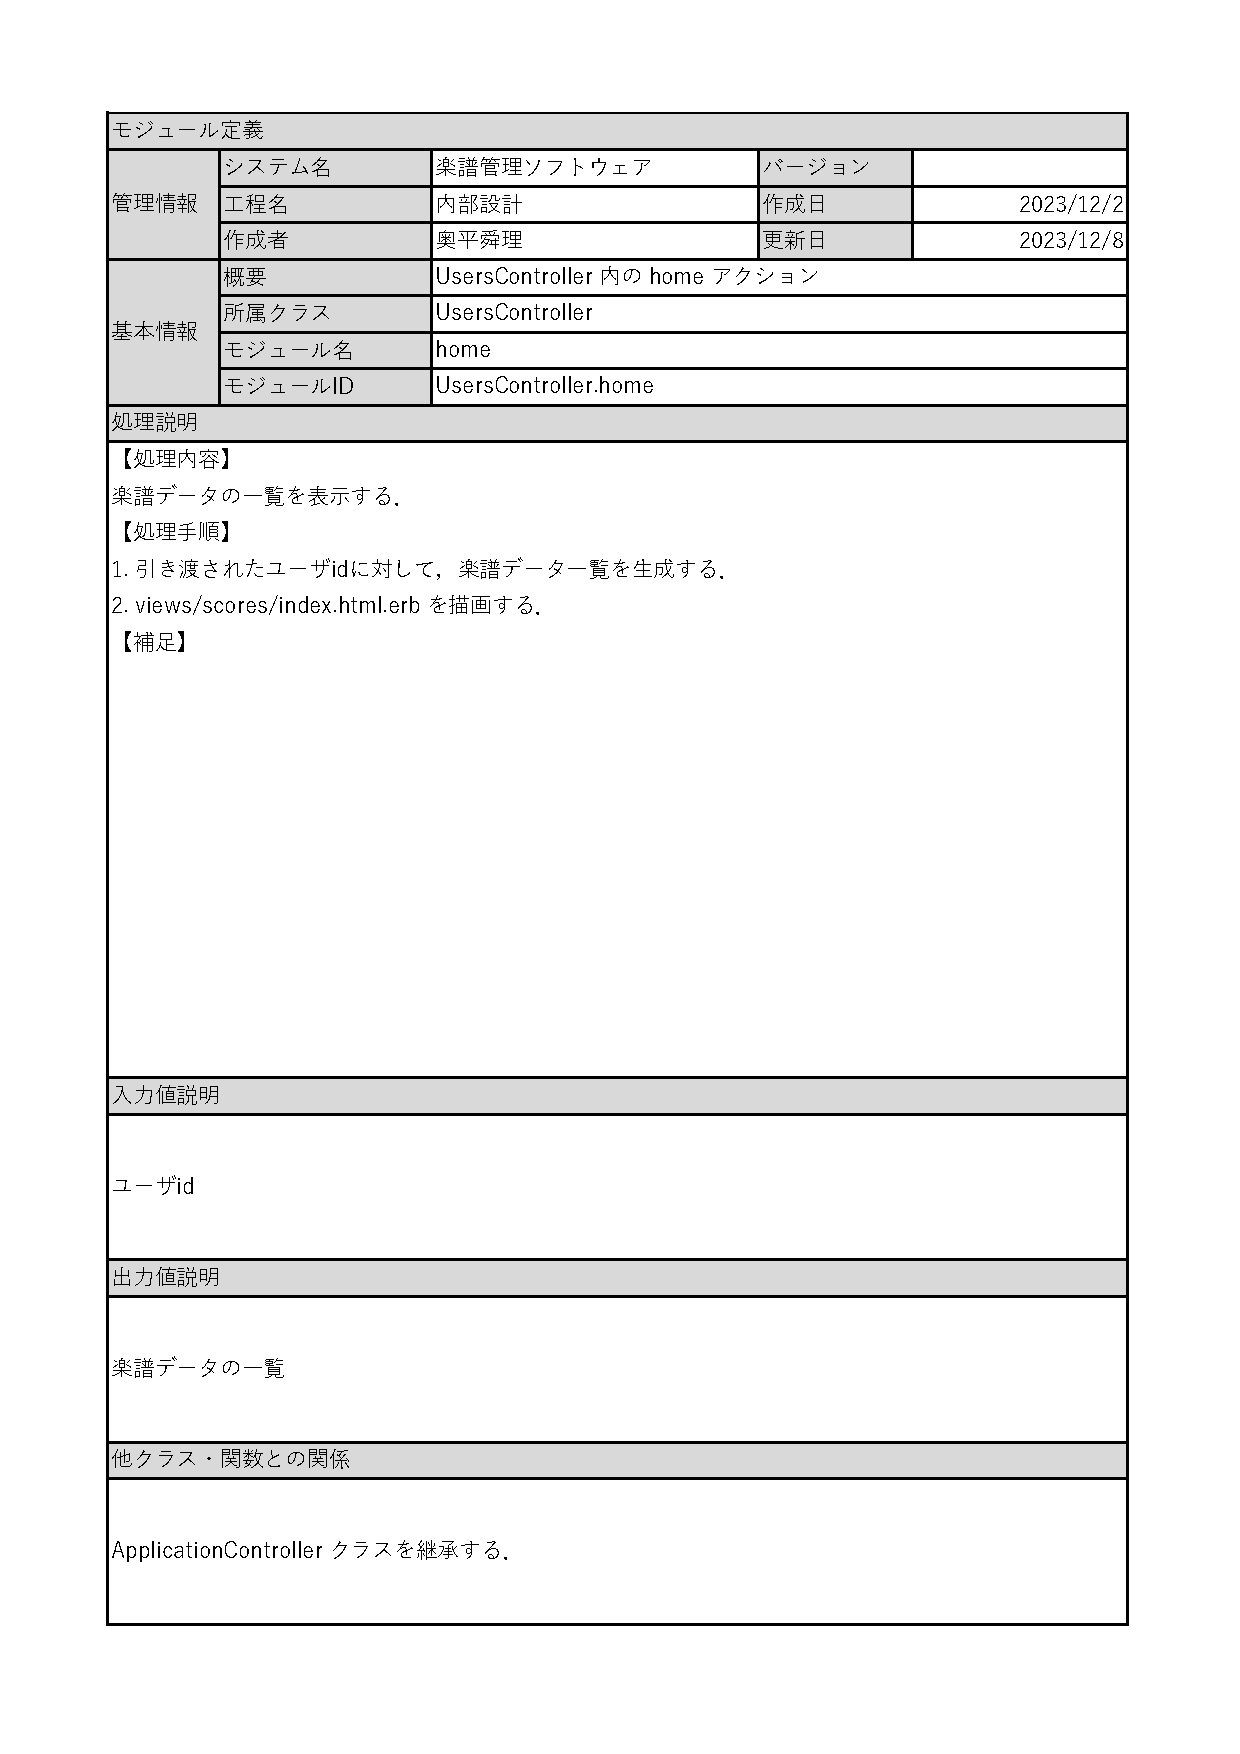
\includegraphics[scale=0.6]{img/Users/xlsx/UsersController_home.pdf}
    \vspace{-1cm}
    \caption{UsersController.home定義書}
\end{figure}
\begin{figure}
    \centering
    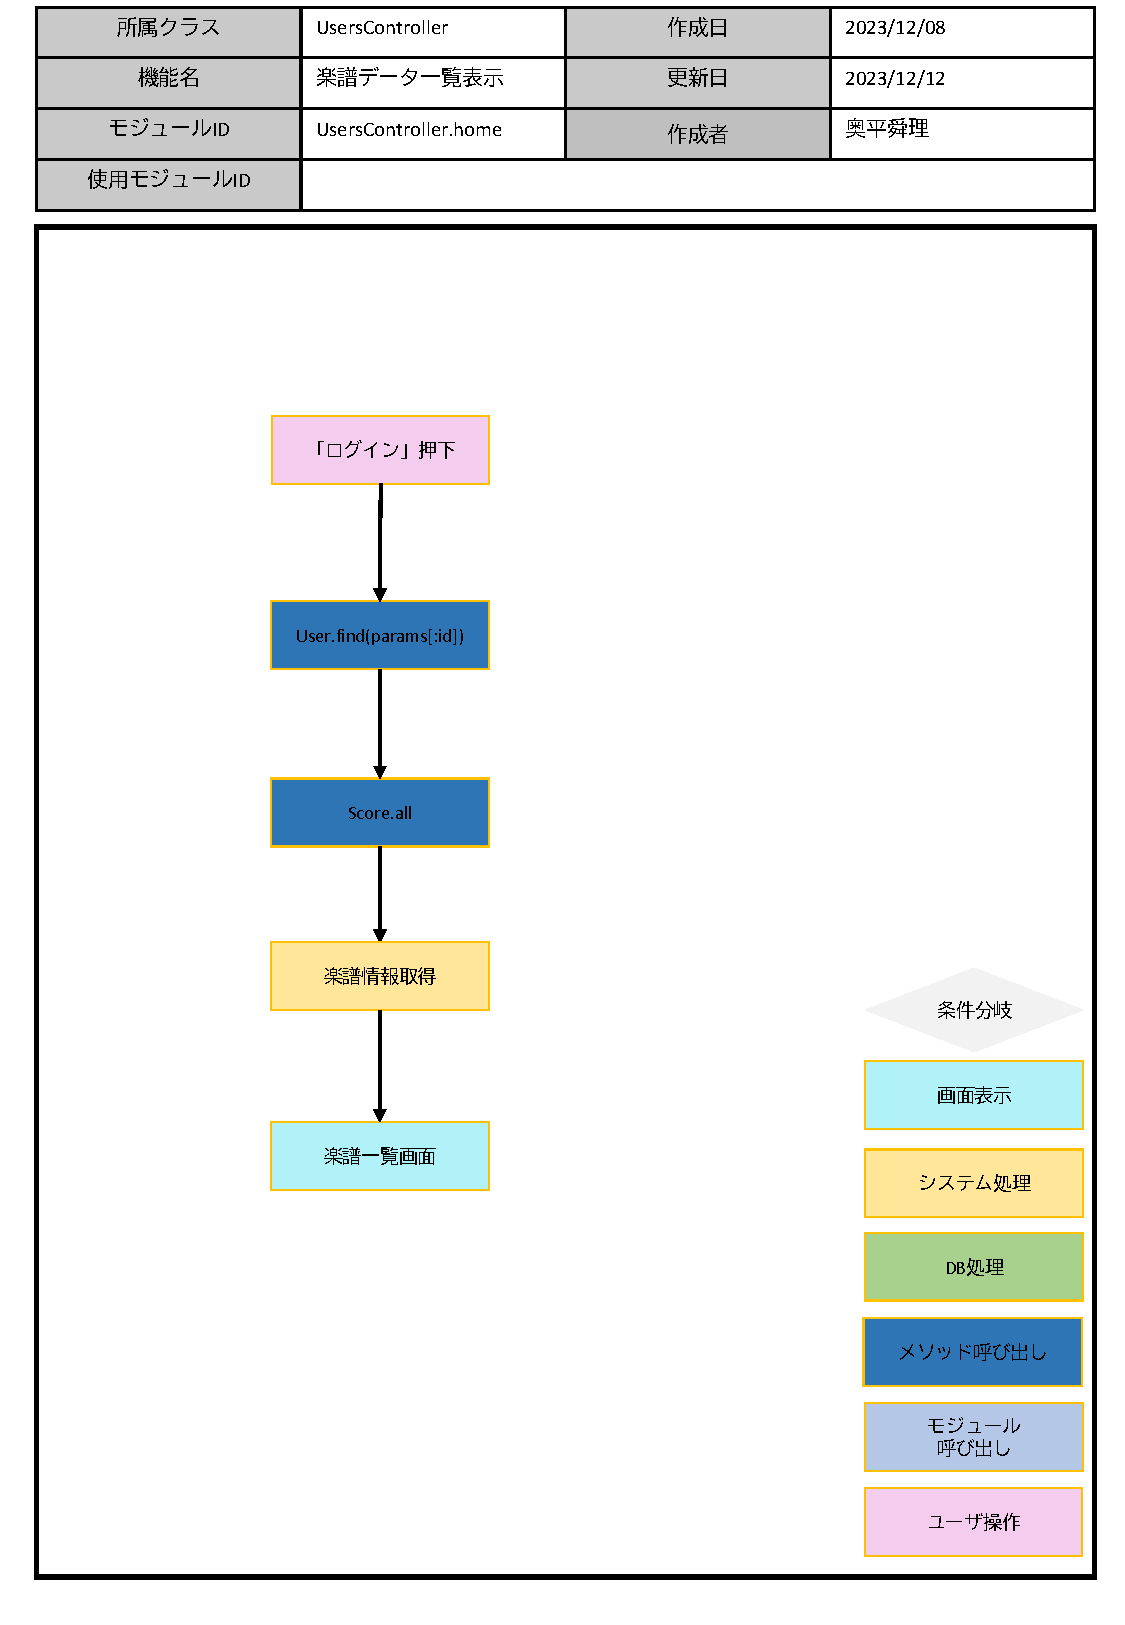
\includegraphics[scale=0.6]{img/Users/pptx/UsersController_home.pdf}
    \caption{UsersController.homeフロー図}
\end{figure}


\clearpage

%show
\subsection*{ScoresController クラスの show アクション}
楽譜の詳細画面を表示する機能を持つ.対応するviewファイルを描画する.
\begin{figure}[H]
    \centering
    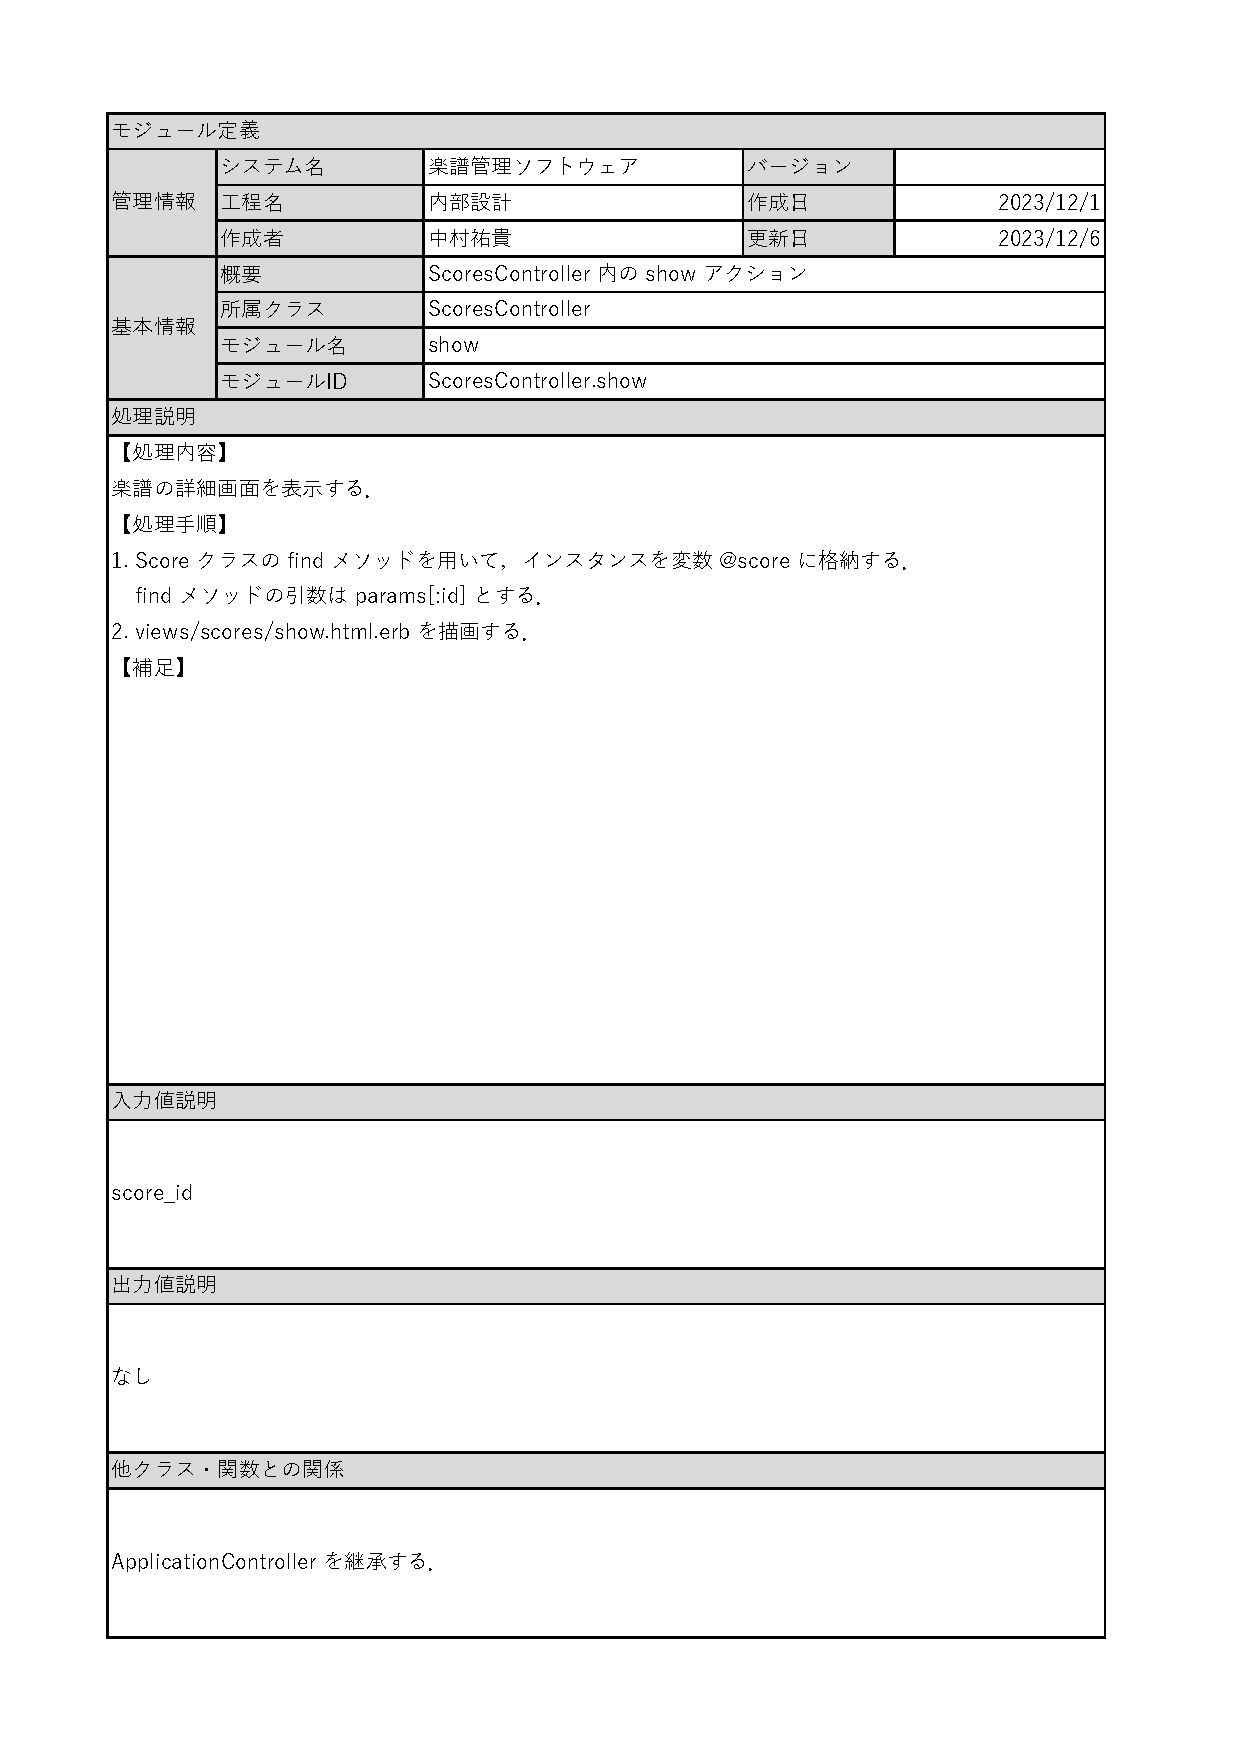
\includegraphics[scale=0.6]{img/Scores/xlsx/ScoresController_show.pdf}
    \vspace{-1cm}
    \caption{ScoresController.show定義書}
\end{figure}
\begin{figure}
    \centering
    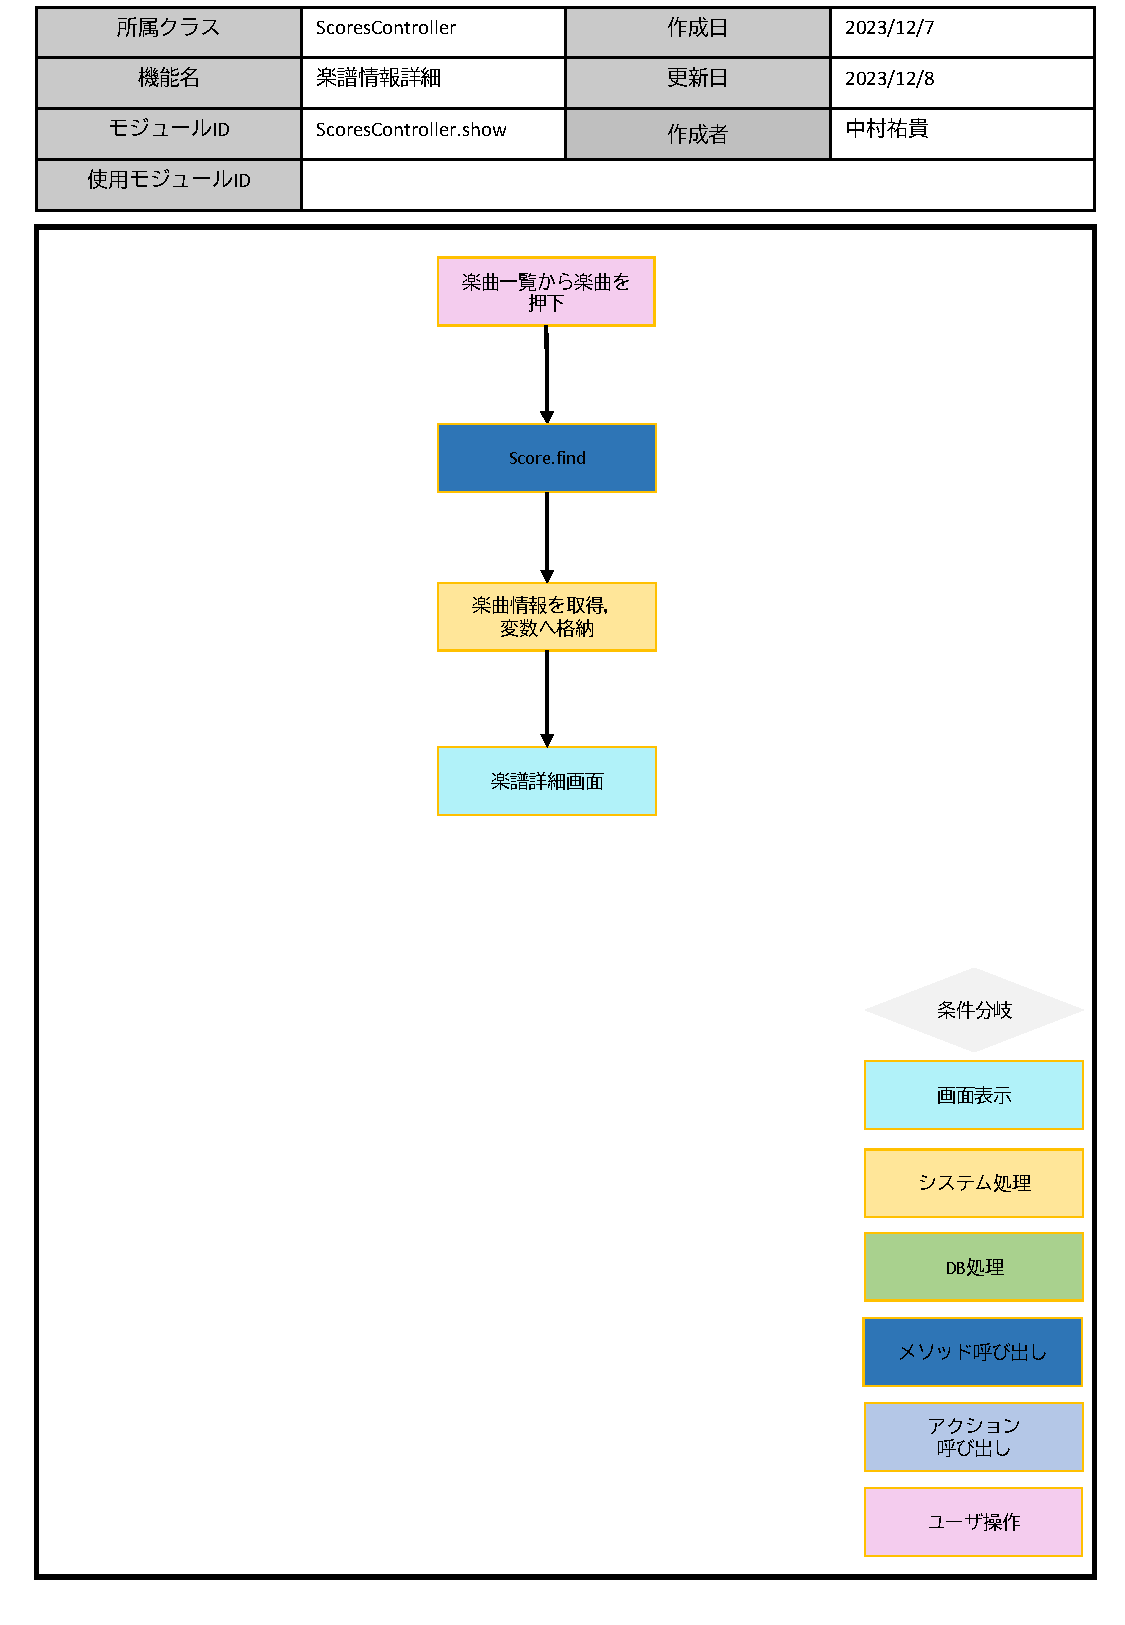
\includegraphics[scale=0.6]{img/Scores/pptx/ScoresController_show.pdf}
    \caption{ScoresController.showフロー図}
\end{figure}
\clearpage
\subsection*{UsersController クラスの show アクション}
ユーザの詳細画面を表示する機能を持つ.対応するviewファイルを描画する.
\begin{figure}[H]
    \centering
    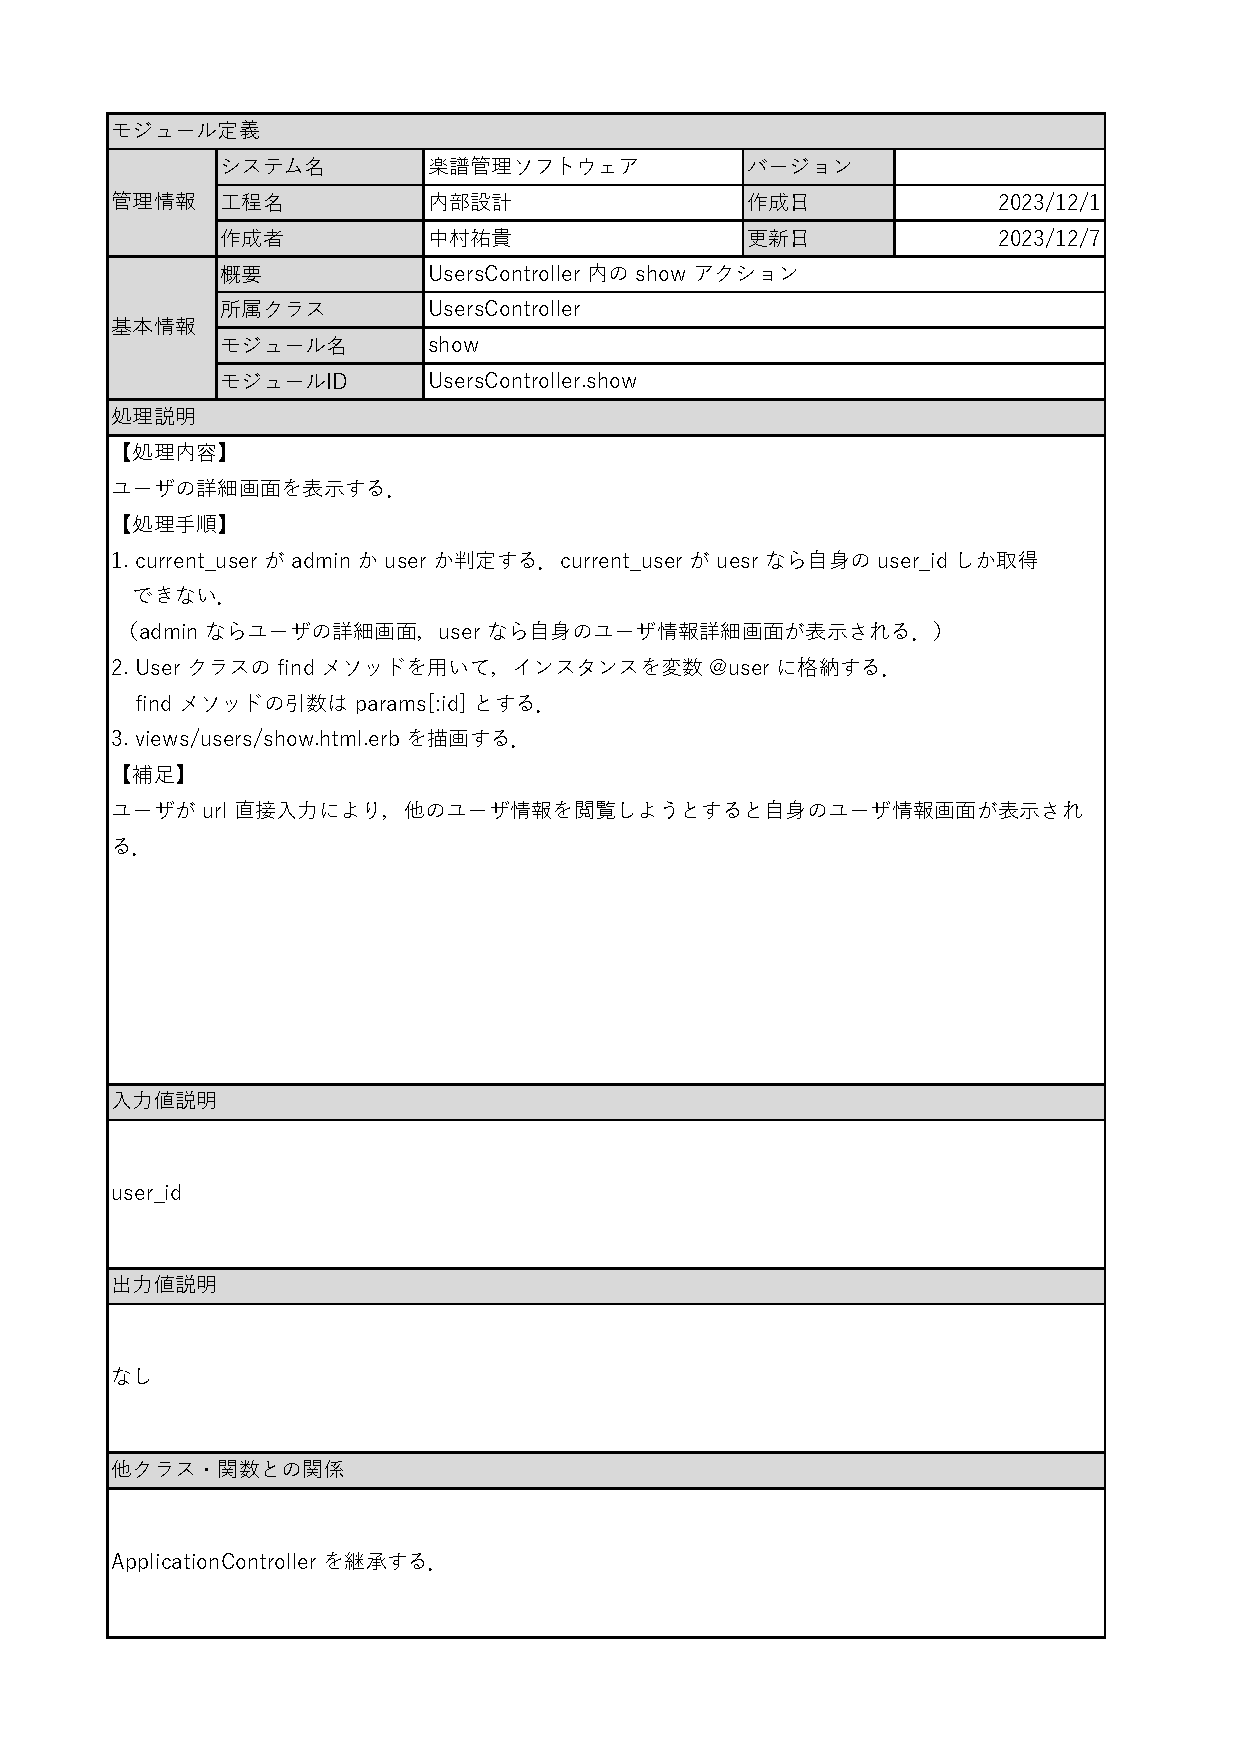
\includegraphics[scale=0.5]{img/Users/xlsx/UsersController_show.pdf}
    \vspace{-0.3cm}
    \caption{UsersController.show定義書}
\end{figure}
\begin{figure}
    \centering
    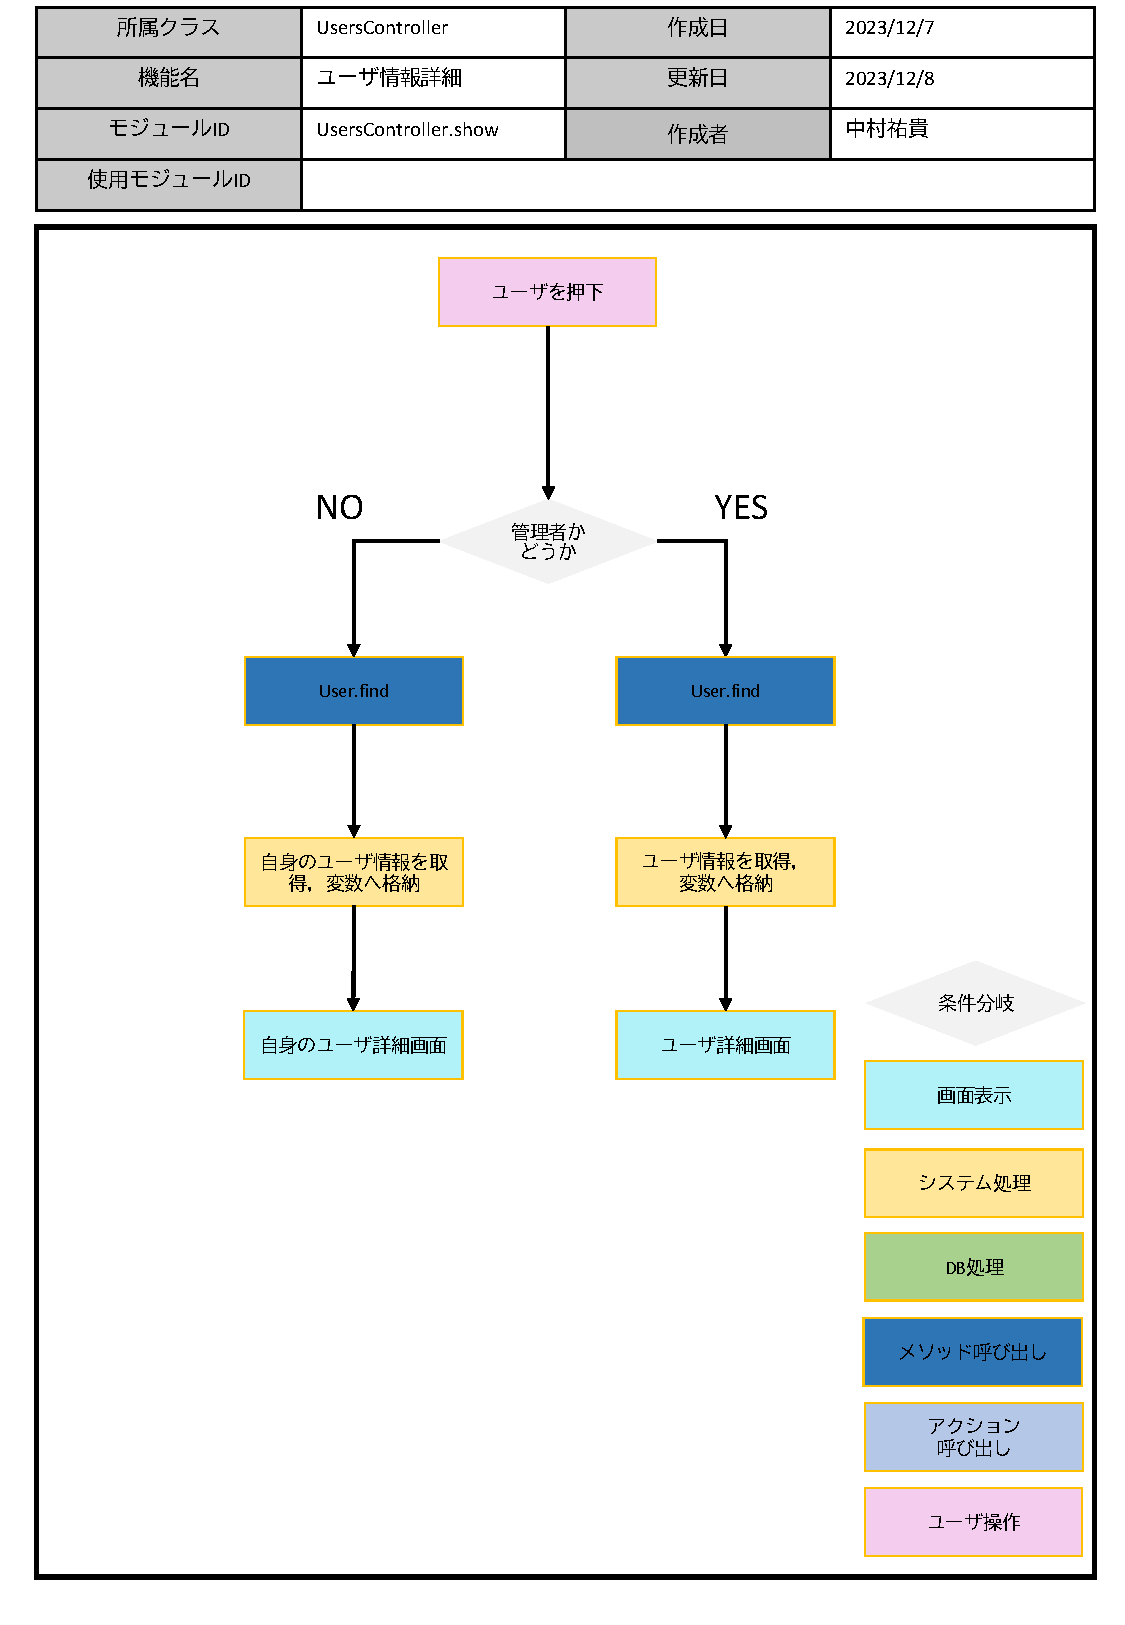
\includegraphics[scale=0.6]{img/Users/pptx/UsersController_show.pdf}
    \vspace{-0.3cm}
    \caption{UsersController.showフロー図}
\end{figure}


\clearpage

%new
\subsection*{ScoresController クラスの new アクション}
楽譜データの新規登録画面を表示する機能を持つ.対応するviewファイルを描画する.
\begin{figure}[H]
    \centering
    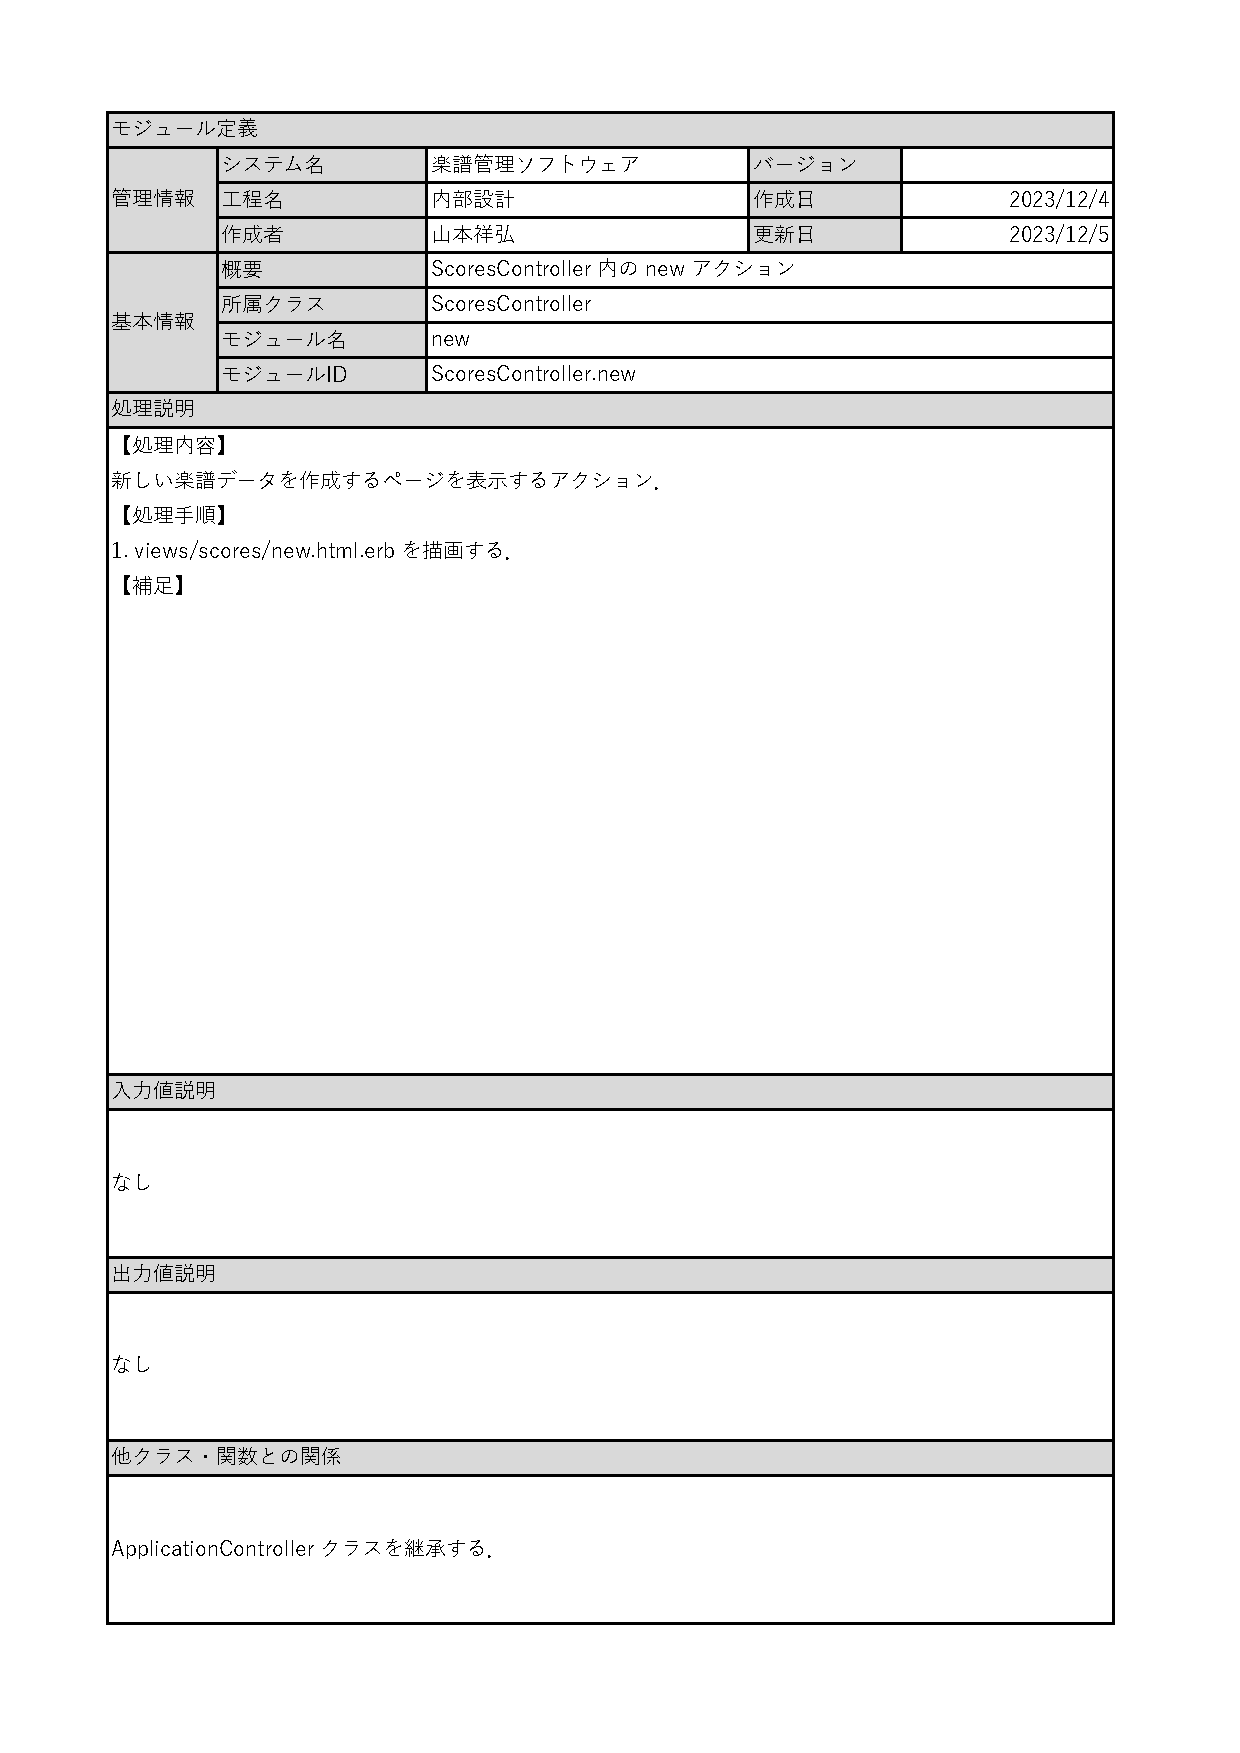
\includegraphics[scale=0.6]{img/Scores/xlsx/ScoresController_new.pdf}
    \vspace{-1cm}
    \caption{ScoresController.new定義書}
\end{figure}
\begin{figure}
    \centering
    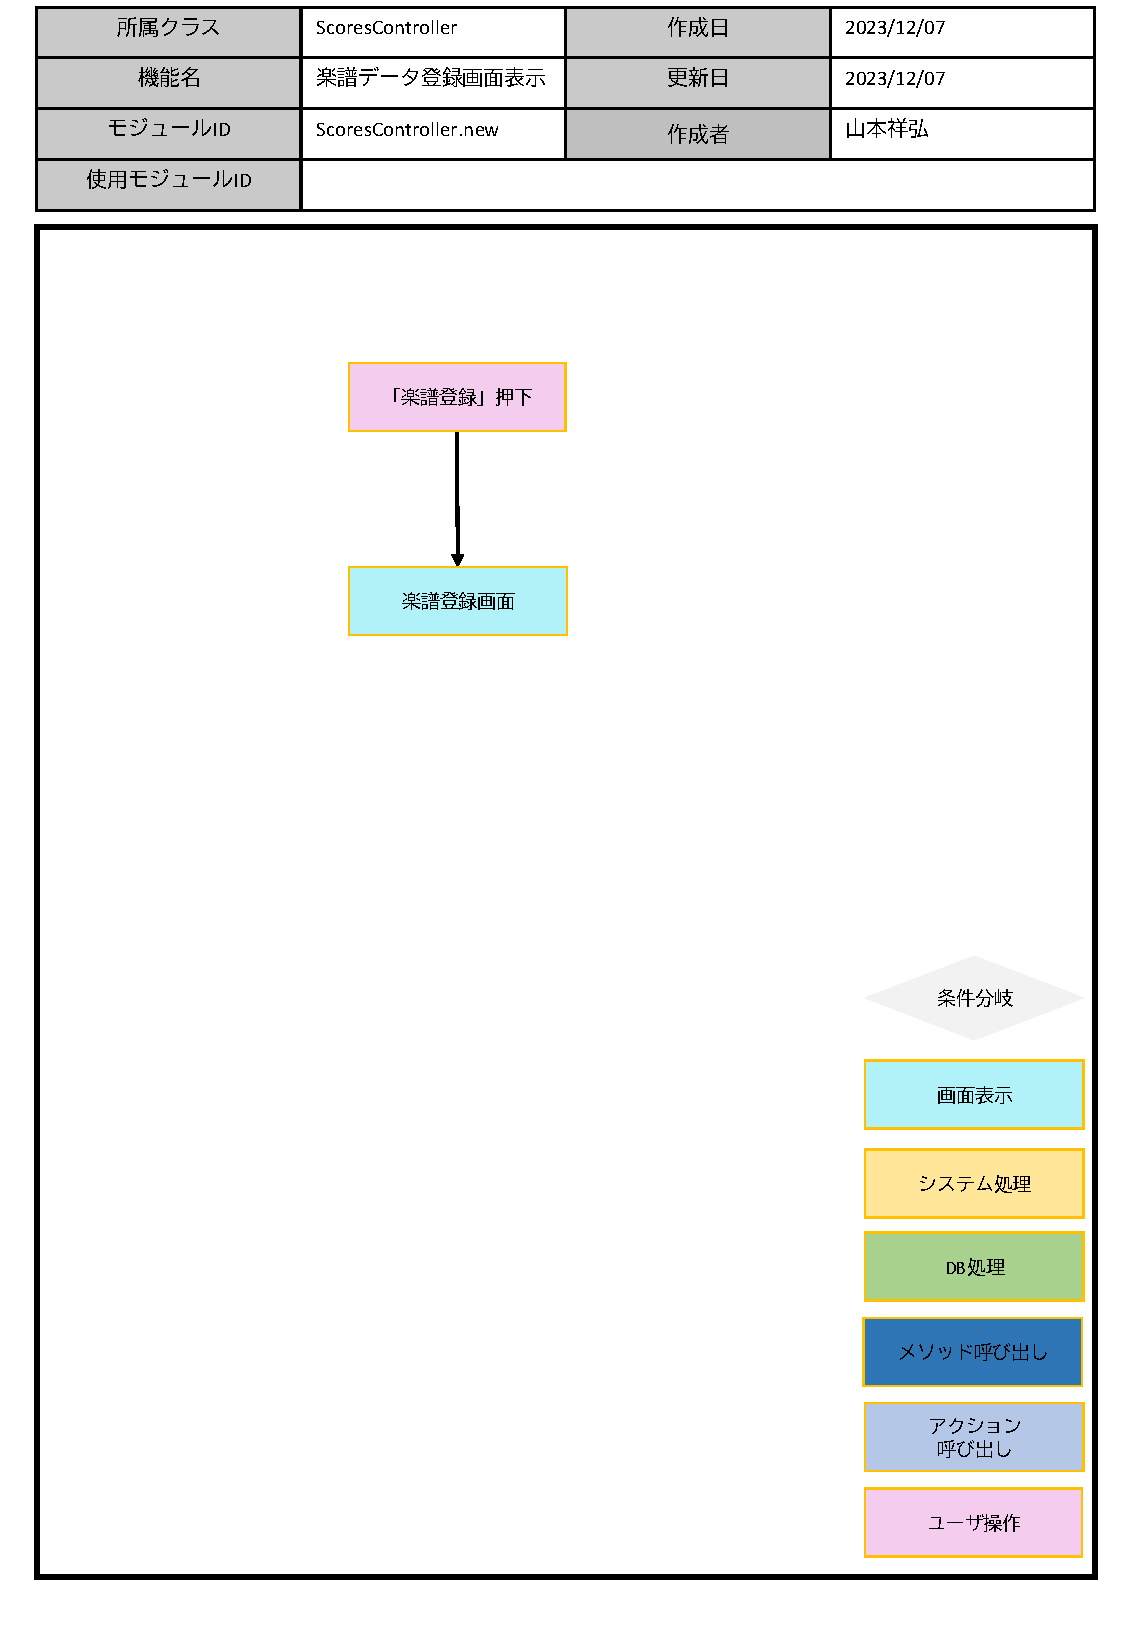
\includegraphics[scale=0.6]{img/Scores/pptx/ScoresController_new.pdf}
    \caption{ScoresController.newフロー図}
\end{figure}
\clearpage
\subsection*{UsersController クラスの new アクション}
ユーザの新規登録画面を表示する機能を持つ.対応するviewファイルを描画する.
\begin{figure}[H]
    \centering
    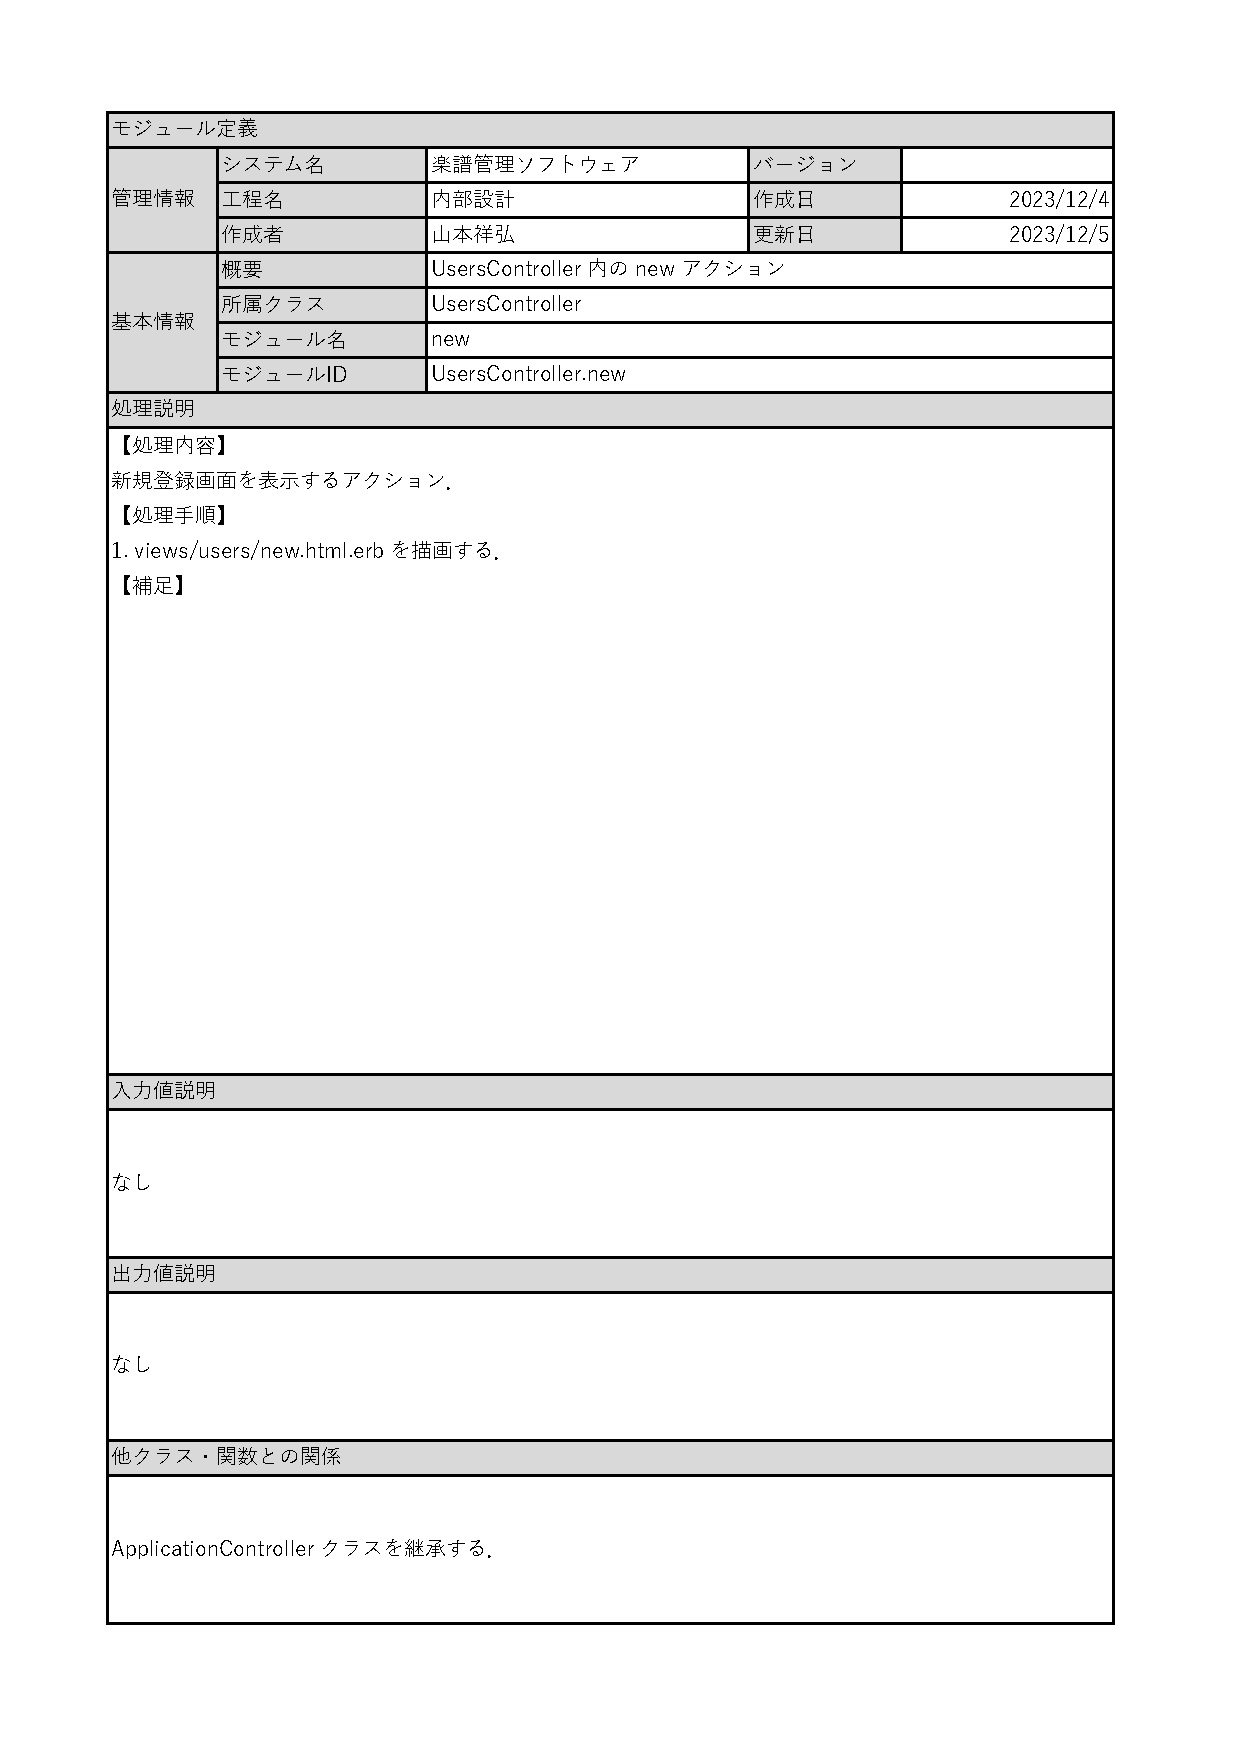
\includegraphics[scale=0.6]{img/Users/xlsx/UsersController_new.pdf}
    \vspace{-1cm}
    \caption{UsersController.new定義書}
\end{figure}
\begin{figure}
    \centering
    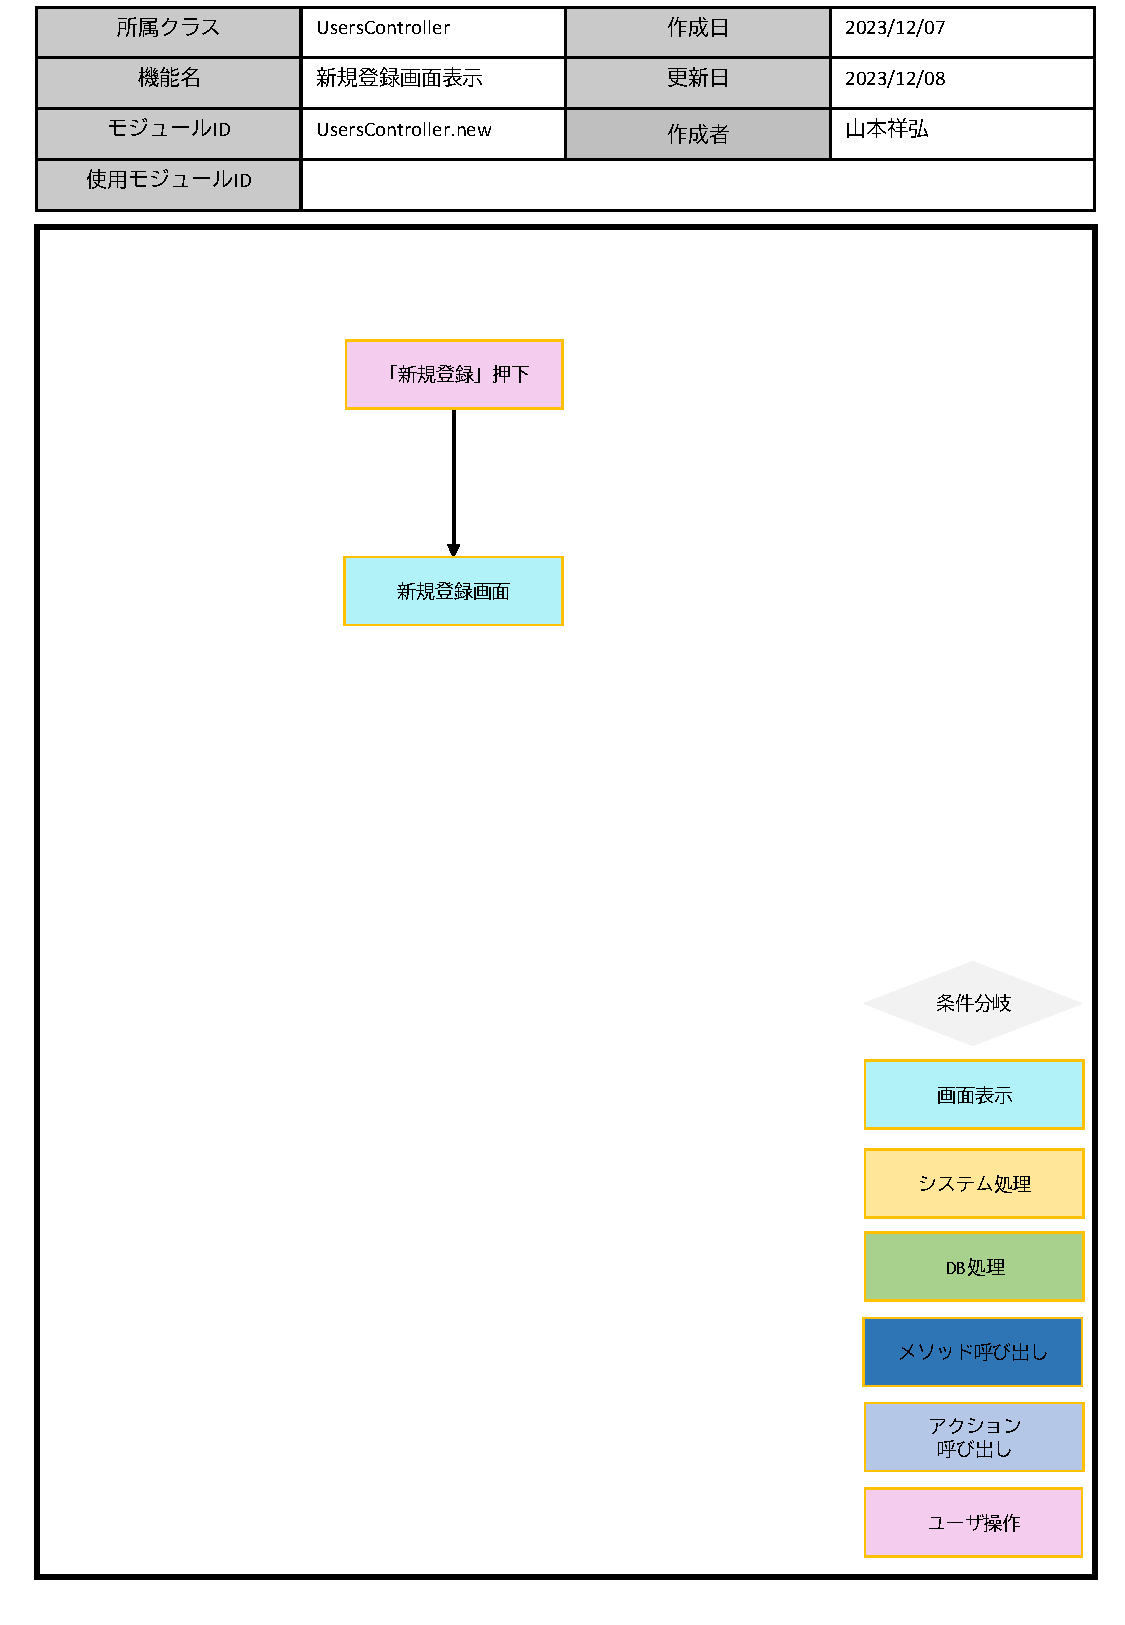
\includegraphics[scale=0.6]{img/Users/pptx/UsersController_new.pdf}
    \caption{UsersController.newフロー図}
\end{figure}


\clearpage

%edit
\subsection*{ScoresController クラスの edit アクション}
既登録された楽譜情報の変種画面を表示する機能を持つ.対応するviewファイルを描画する.
\begin{figure}[H]
    \centering
    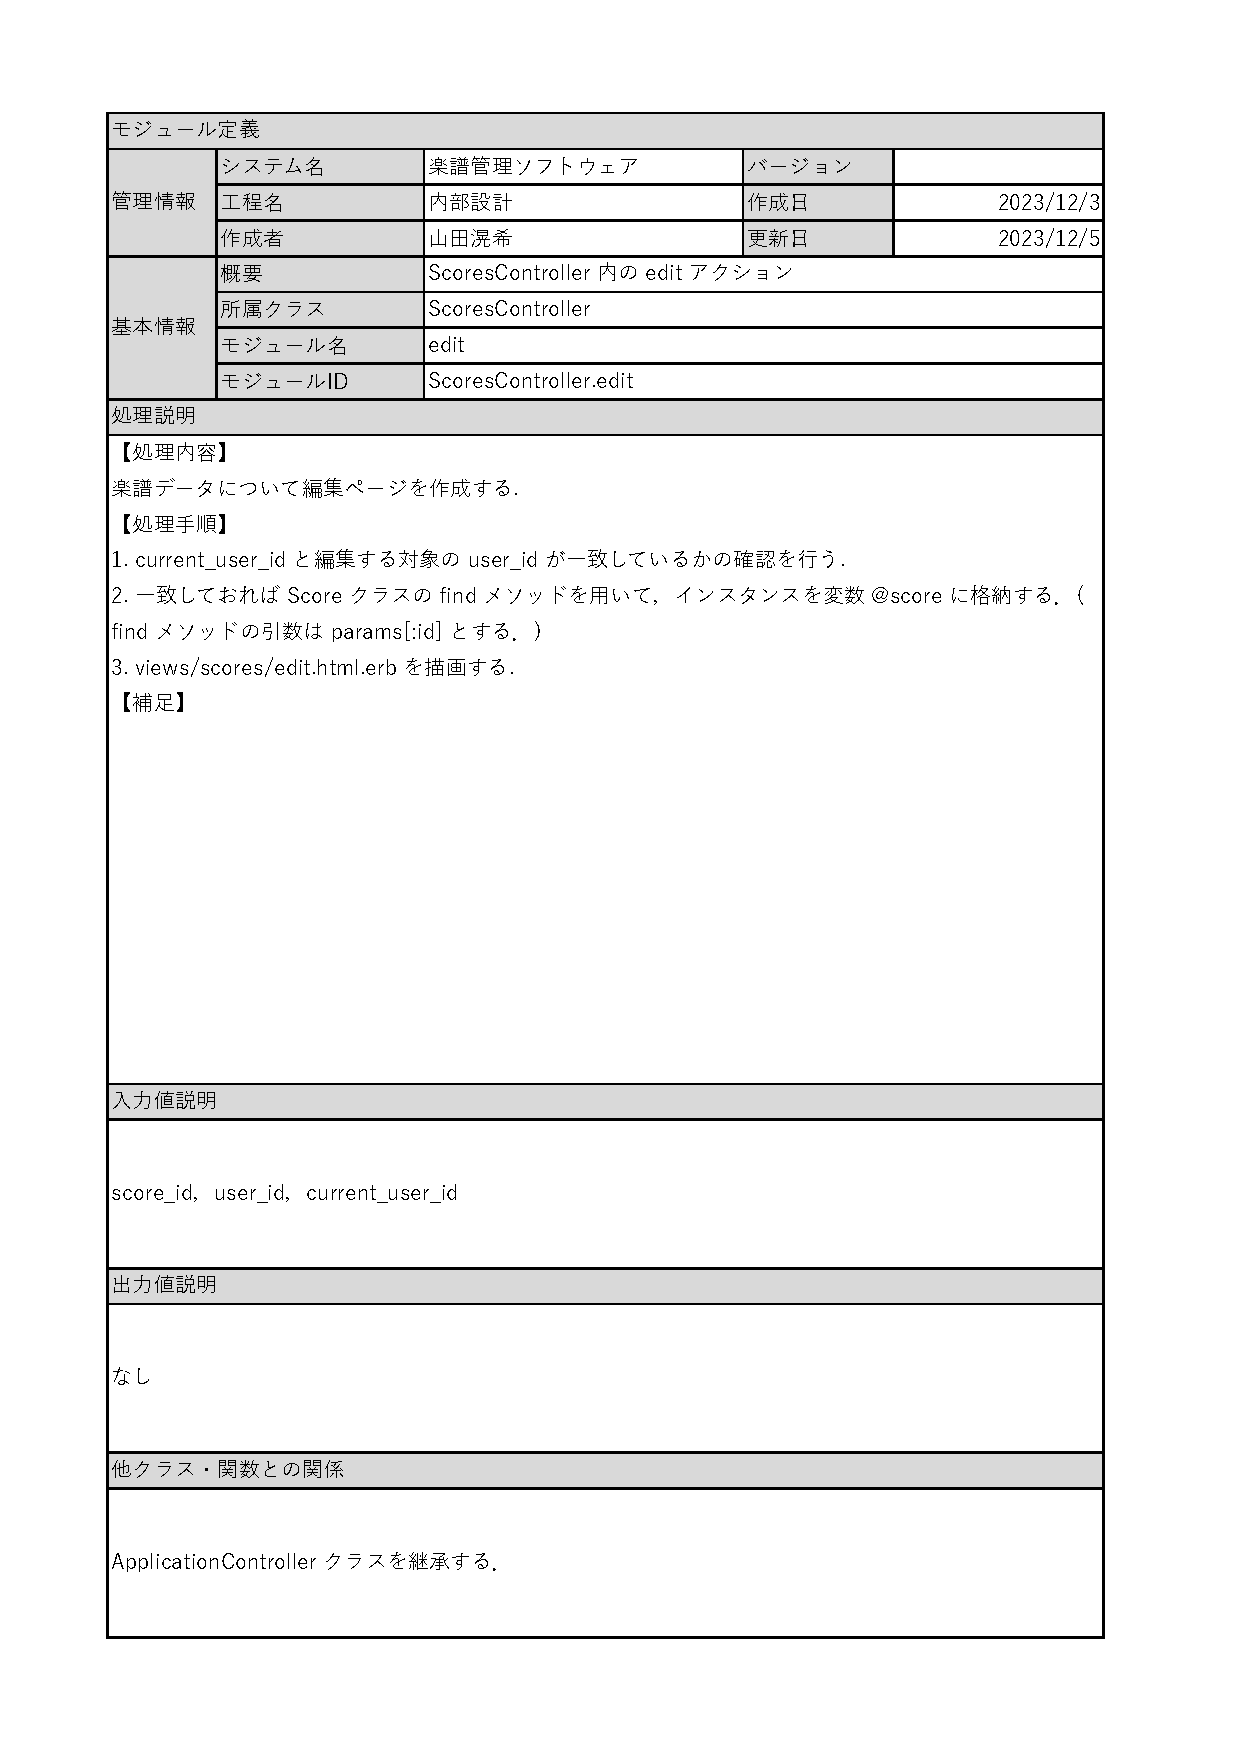
\includegraphics[scale=0.6]{img/Scores/xlsx/ScoresController_edit.pdf}
    \vspace{-1cm}
    \caption{ScoresController.edit定義書}
\end{figure}
\begin{figure}
    \centering
    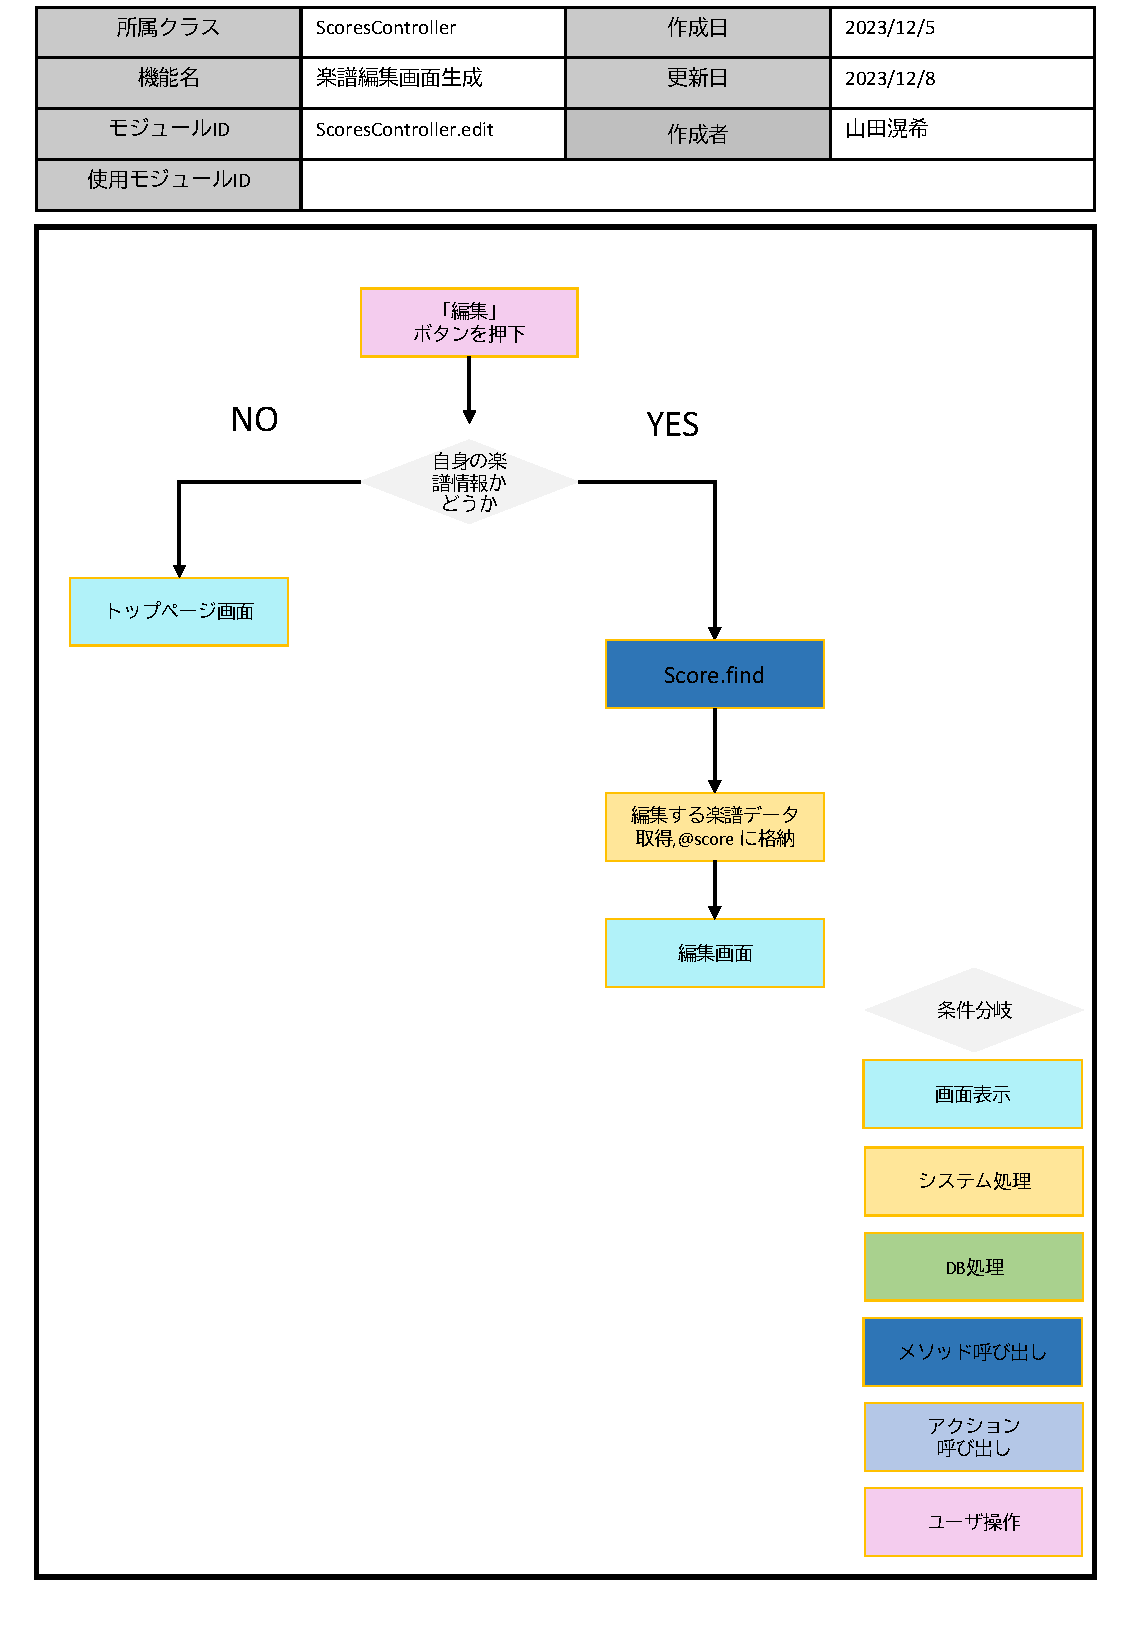
\includegraphics[scale=0.6]{img/Scores/pptx/ScoresController_edit.pdf}
    \caption{ScoresController.editフロー図}
\end{figure}
\clearpage
\subsection*{Userscontroller クラスの edit アクション}
既登録されたユーザ情報を編集する機能を持つ.対応するviewファイルを描画する.
\begin{figure}
    \centering
    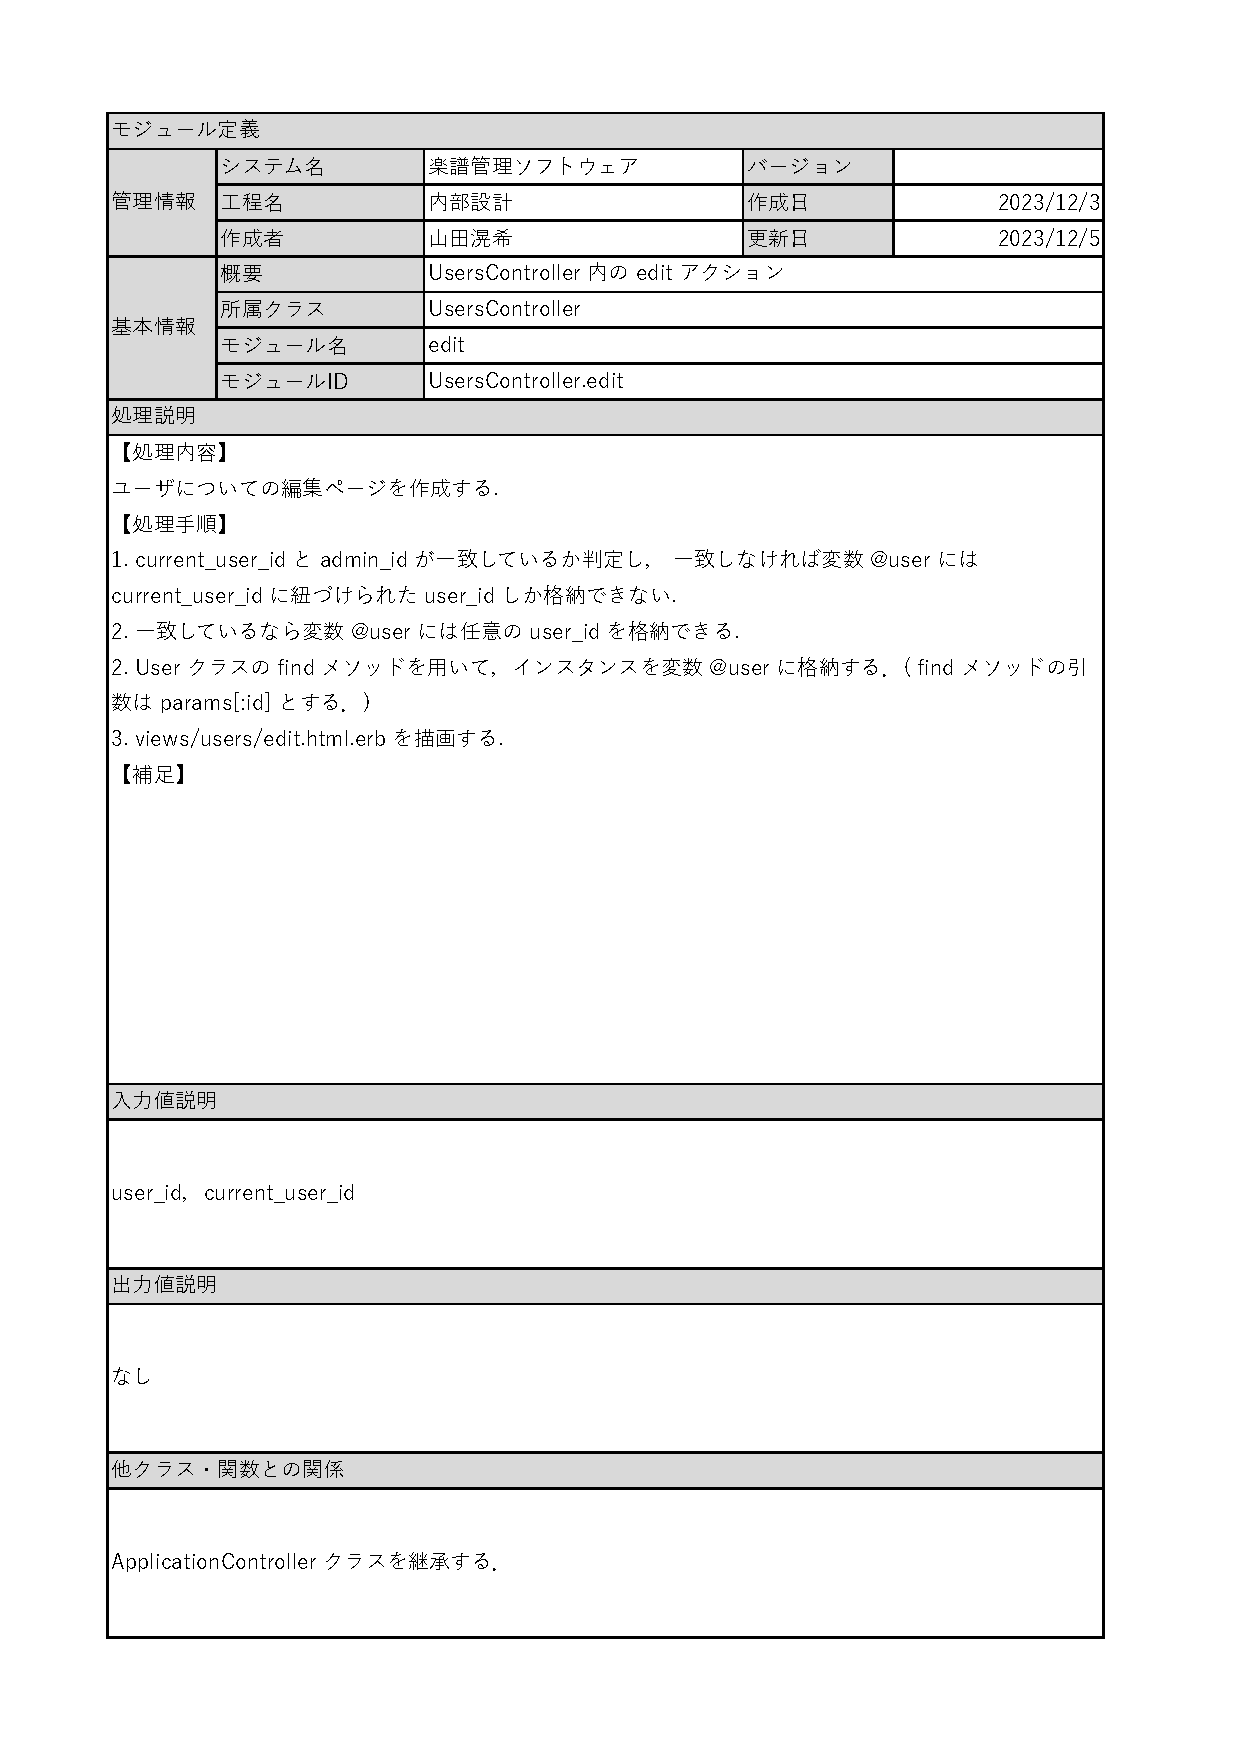
\includegraphics[scale=0.6]{img/Users/xlsx/UsersController_edit.pdf}
    \vspace{-1cm}
    \caption{UsersController.edit定義書}
\end{figure}
\begin{figure}
    \centering
    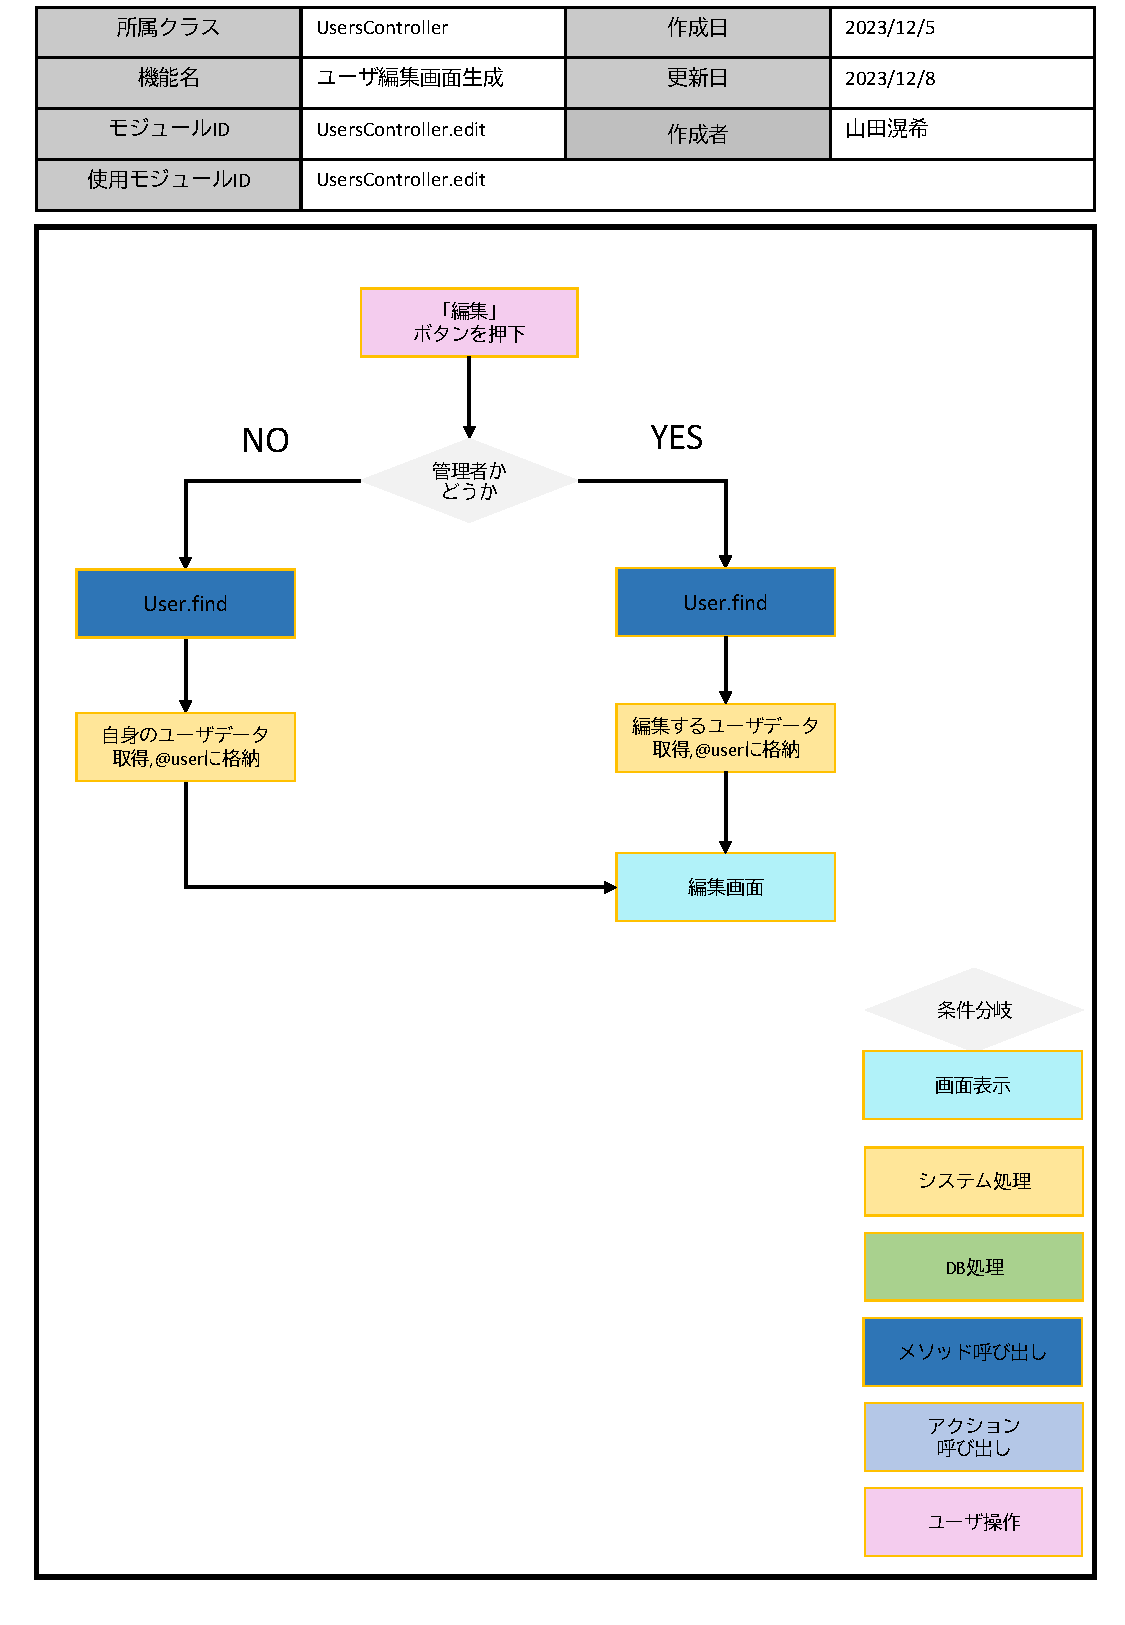
\includegraphics[scale=0.6]{img/Users/pptx/UsersController_edit.pdf}
    \caption{UsersController.editフロー図}
\end{figure}

\clearpage


%create
\subsection*{ScoresController クラスの create アクション}
新規に楽曲を登録する機能を持つ.viewは持たない.
\begin{figure}[H]
    \centering
    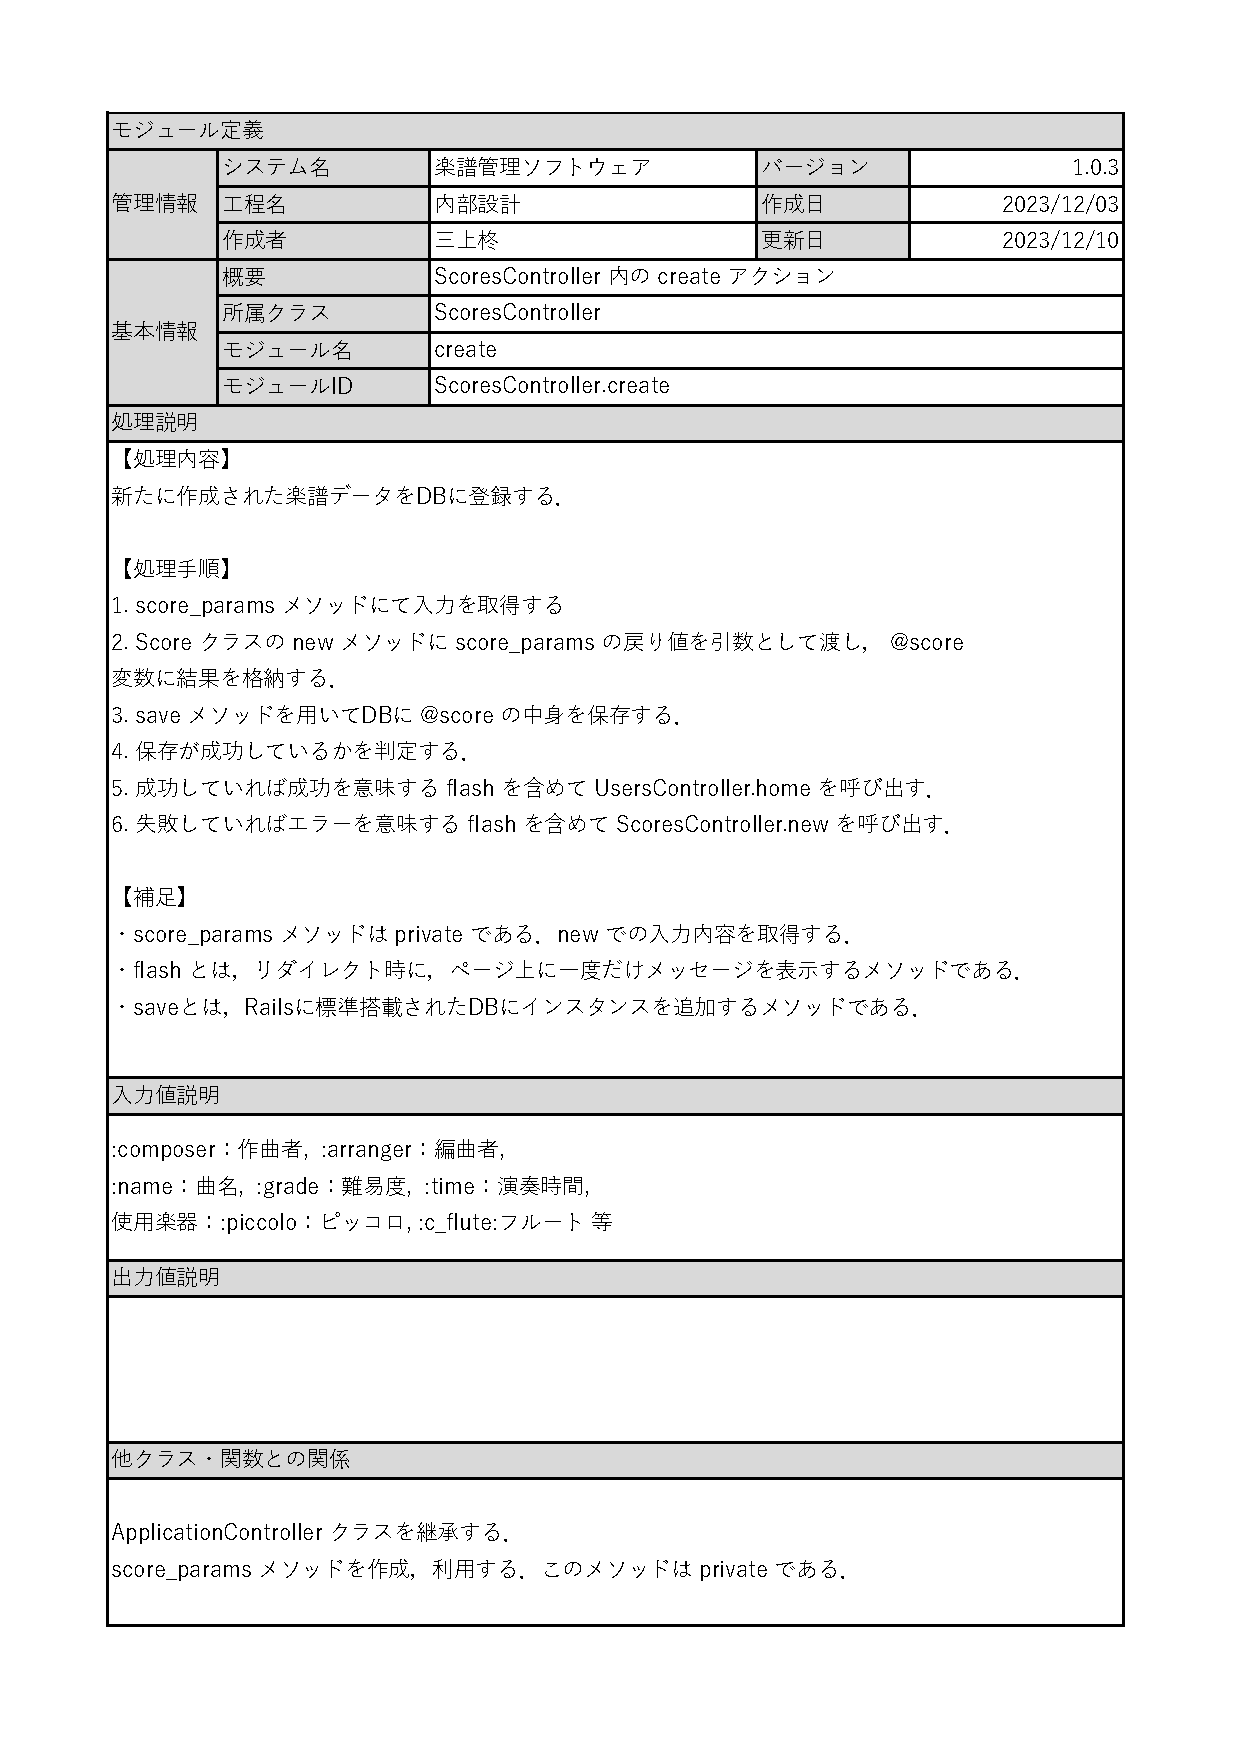
\includegraphics[scale=0.6]{img/Scores/xlsx/ScoresController_create.pdf}
    \vspace{-1cm}
    \caption{ScoresController.create定義書}
\end{figure}
\begin{figure}
    \centering
    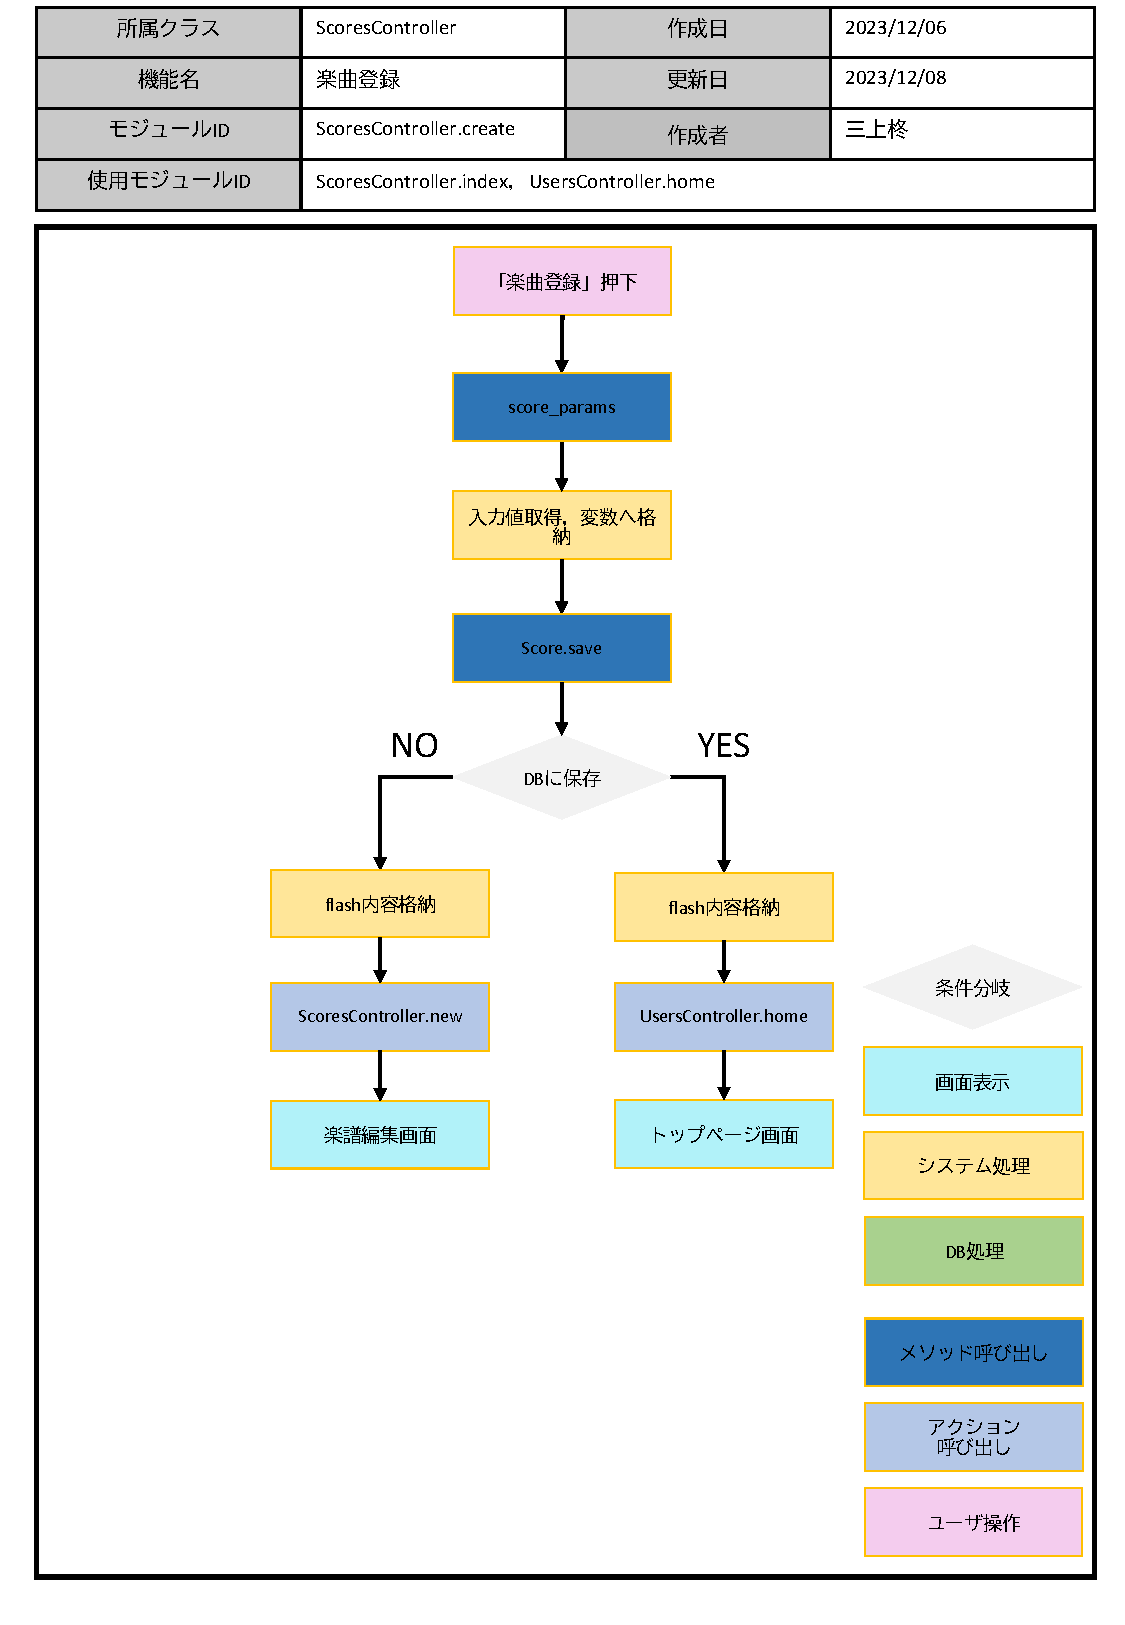
\includegraphics[scale=0.6]{img/Scores/pptx/ScoresController_create.pdf}
    \caption{ScoresController.createフロー図}
\end{figure}
\clearpage
\subsection*{UsersController クラスの create アクション}
新規のユーザを登録する機能を持つ.viewは持たない.
\begin{figure}[H]
    \centering
    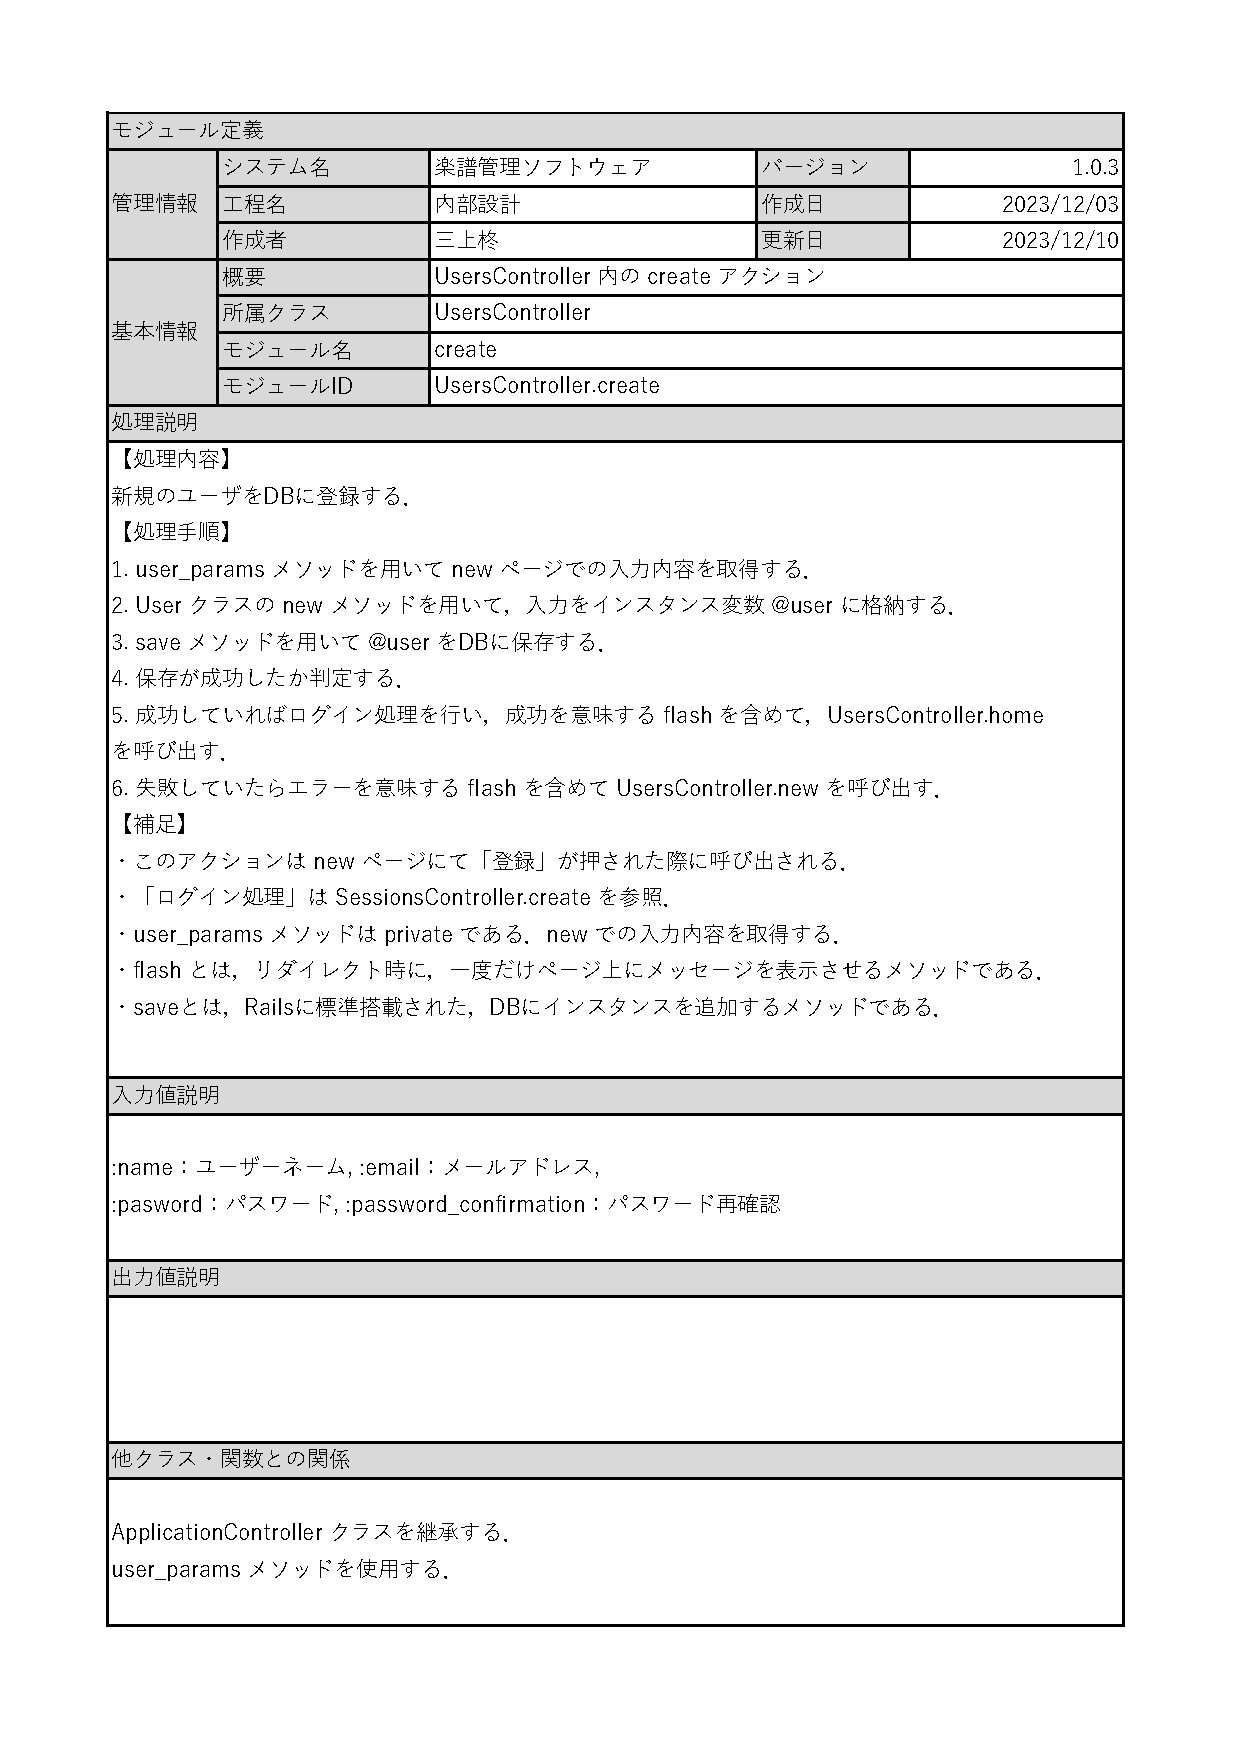
\includegraphics[scale=0.6]{img/Users/xlsx/UsersController_create.pdf}
    \vspace{-1cm}
    \caption{UsersController.create定義書}
\end{figure}
\begin{figure}
    \centering
    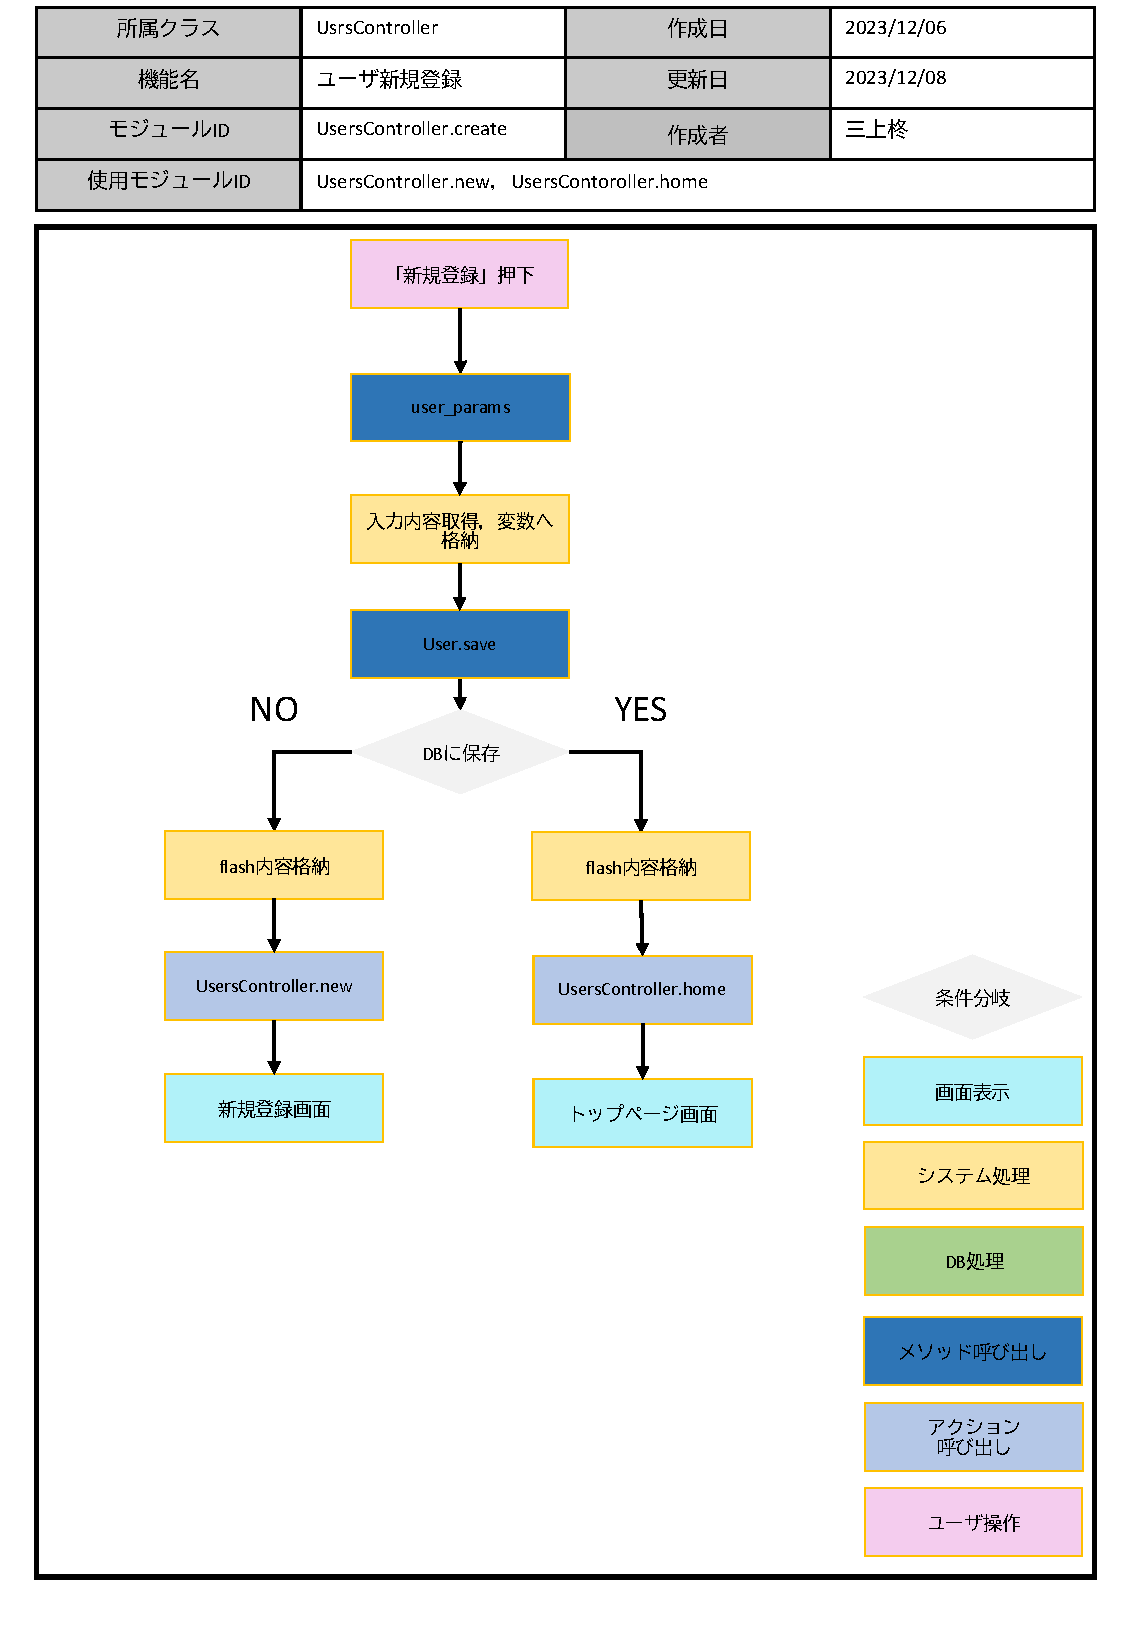
\includegraphics[scale=0.6]{img/Users/pptx/UsersController_create.pdf}
    \caption{UsersController.createフロー図}
\end{figure}

\clearpage

%create
\subsection*{ScoresController クラスの update アクション}
既登録された楽譜の編集情報をDBに更新する機能を持つ.viewは持たない.
\begin{figure}[H]
    \centering
    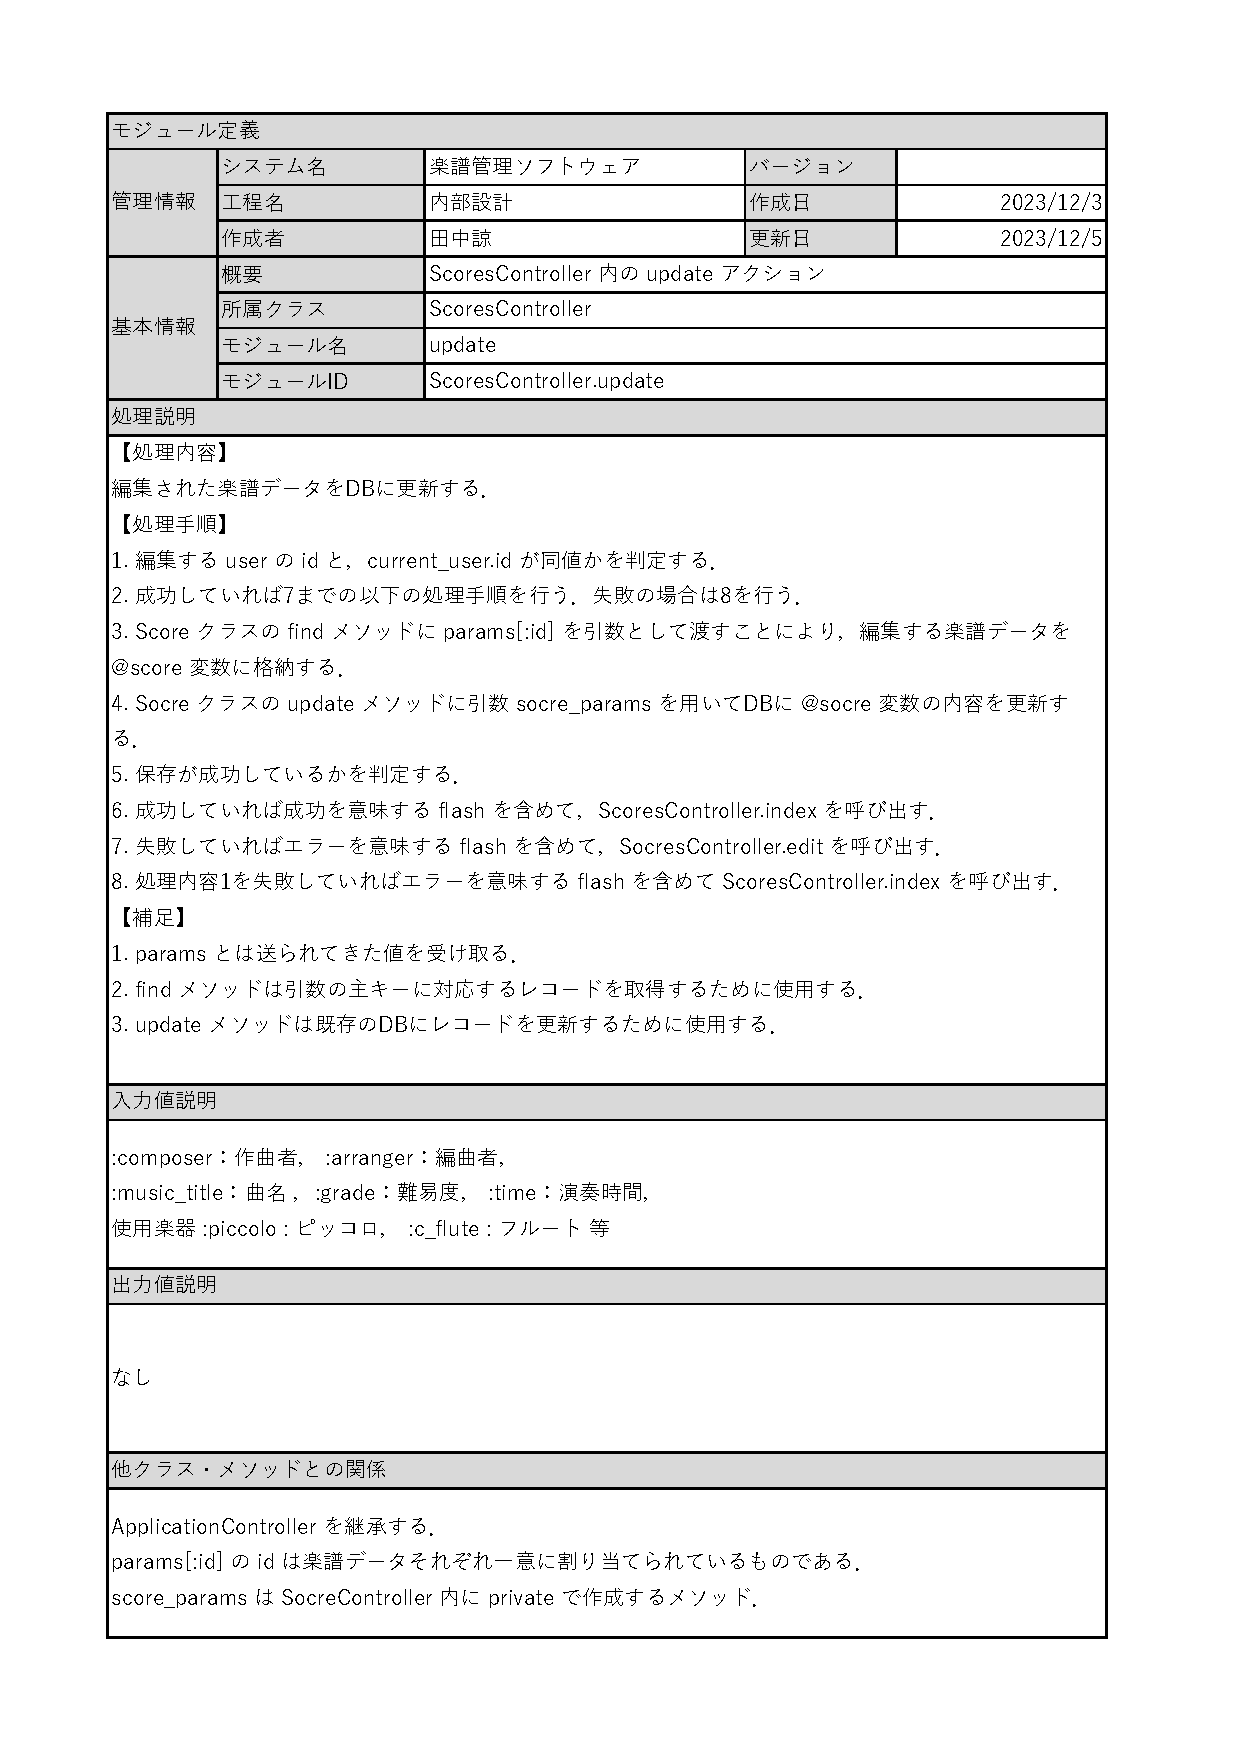
\includegraphics[scale=0.6]{img/Scores/xlsx/ScoresController_update.pdf}
    \vspace{-1cm}
    \caption{ScoresController.update定義書}
\end{figure}
\begin{figure}
    \centering
    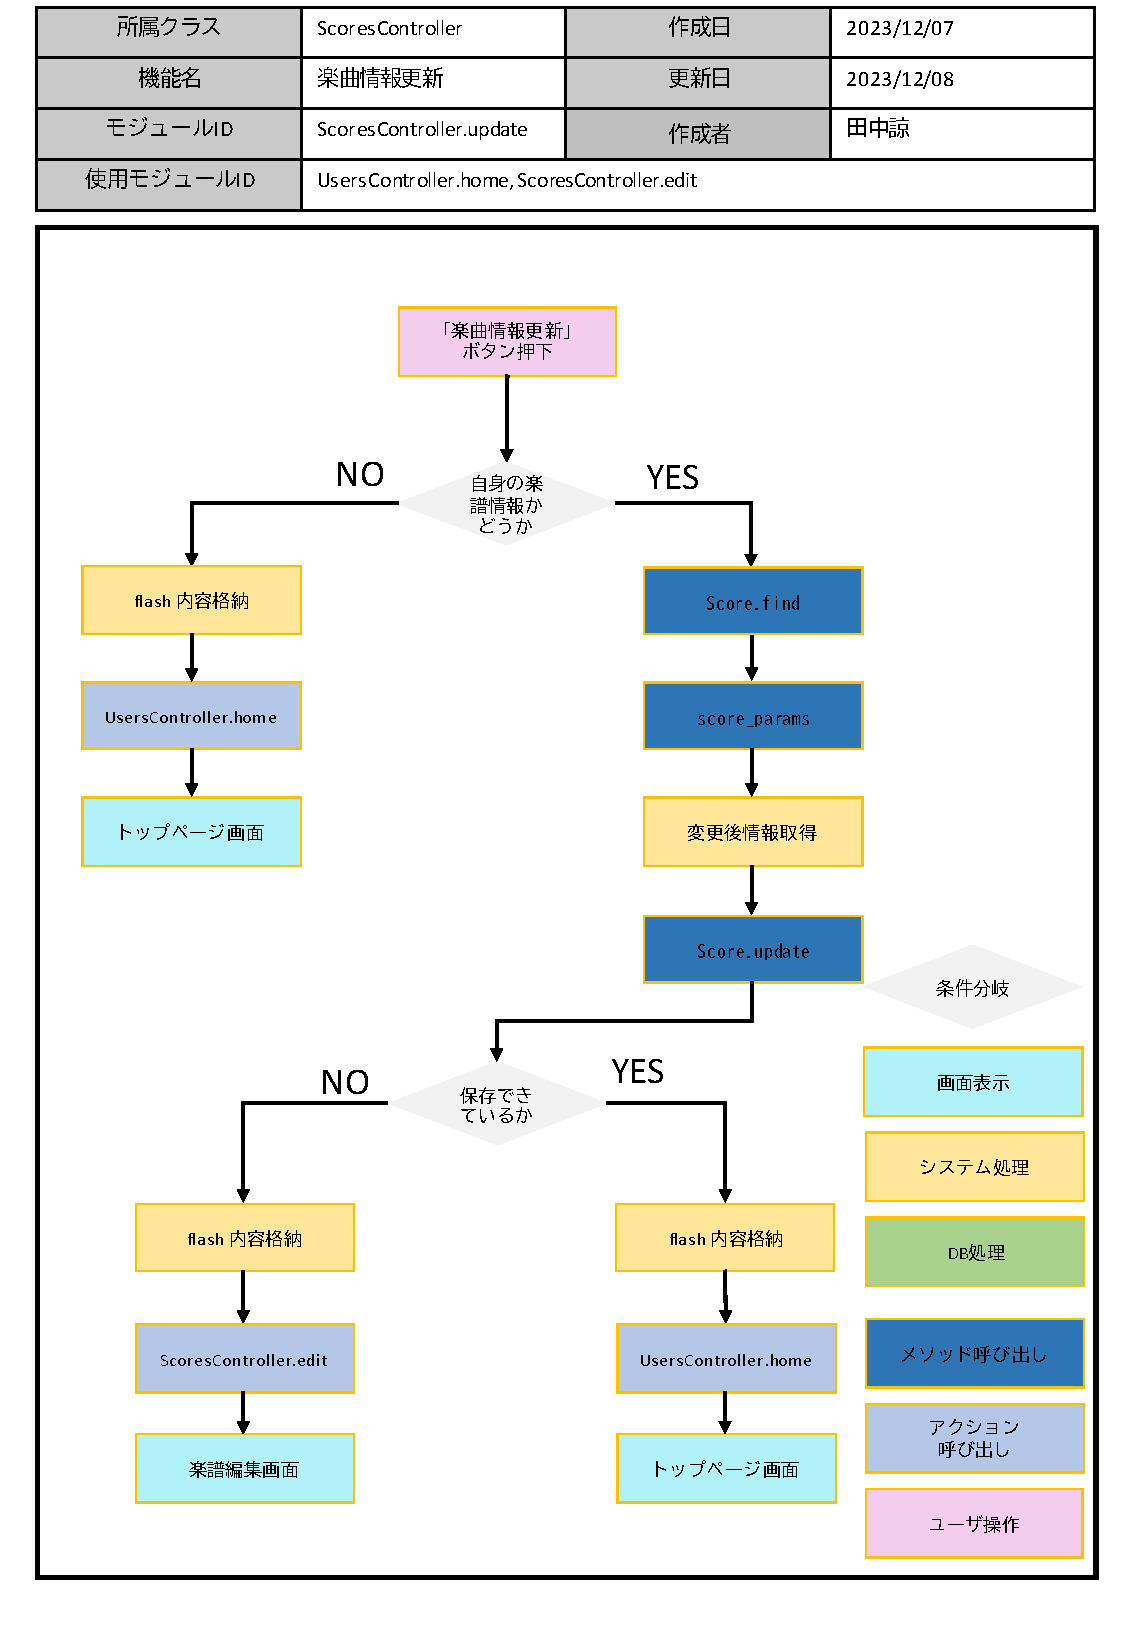
\includegraphics[scale=0.6]{img/Scores/pptx/ScoresController_update.pdf}
    \caption{ScoresController.updateフロー図}
\end{figure}
\clearpage
\subsection*{UsersController クラスの update アクション}
既登録されたユーザの編集情報をDBに更新する機能を持つ.viewは持たない.
\begin{figure}
    \centering
    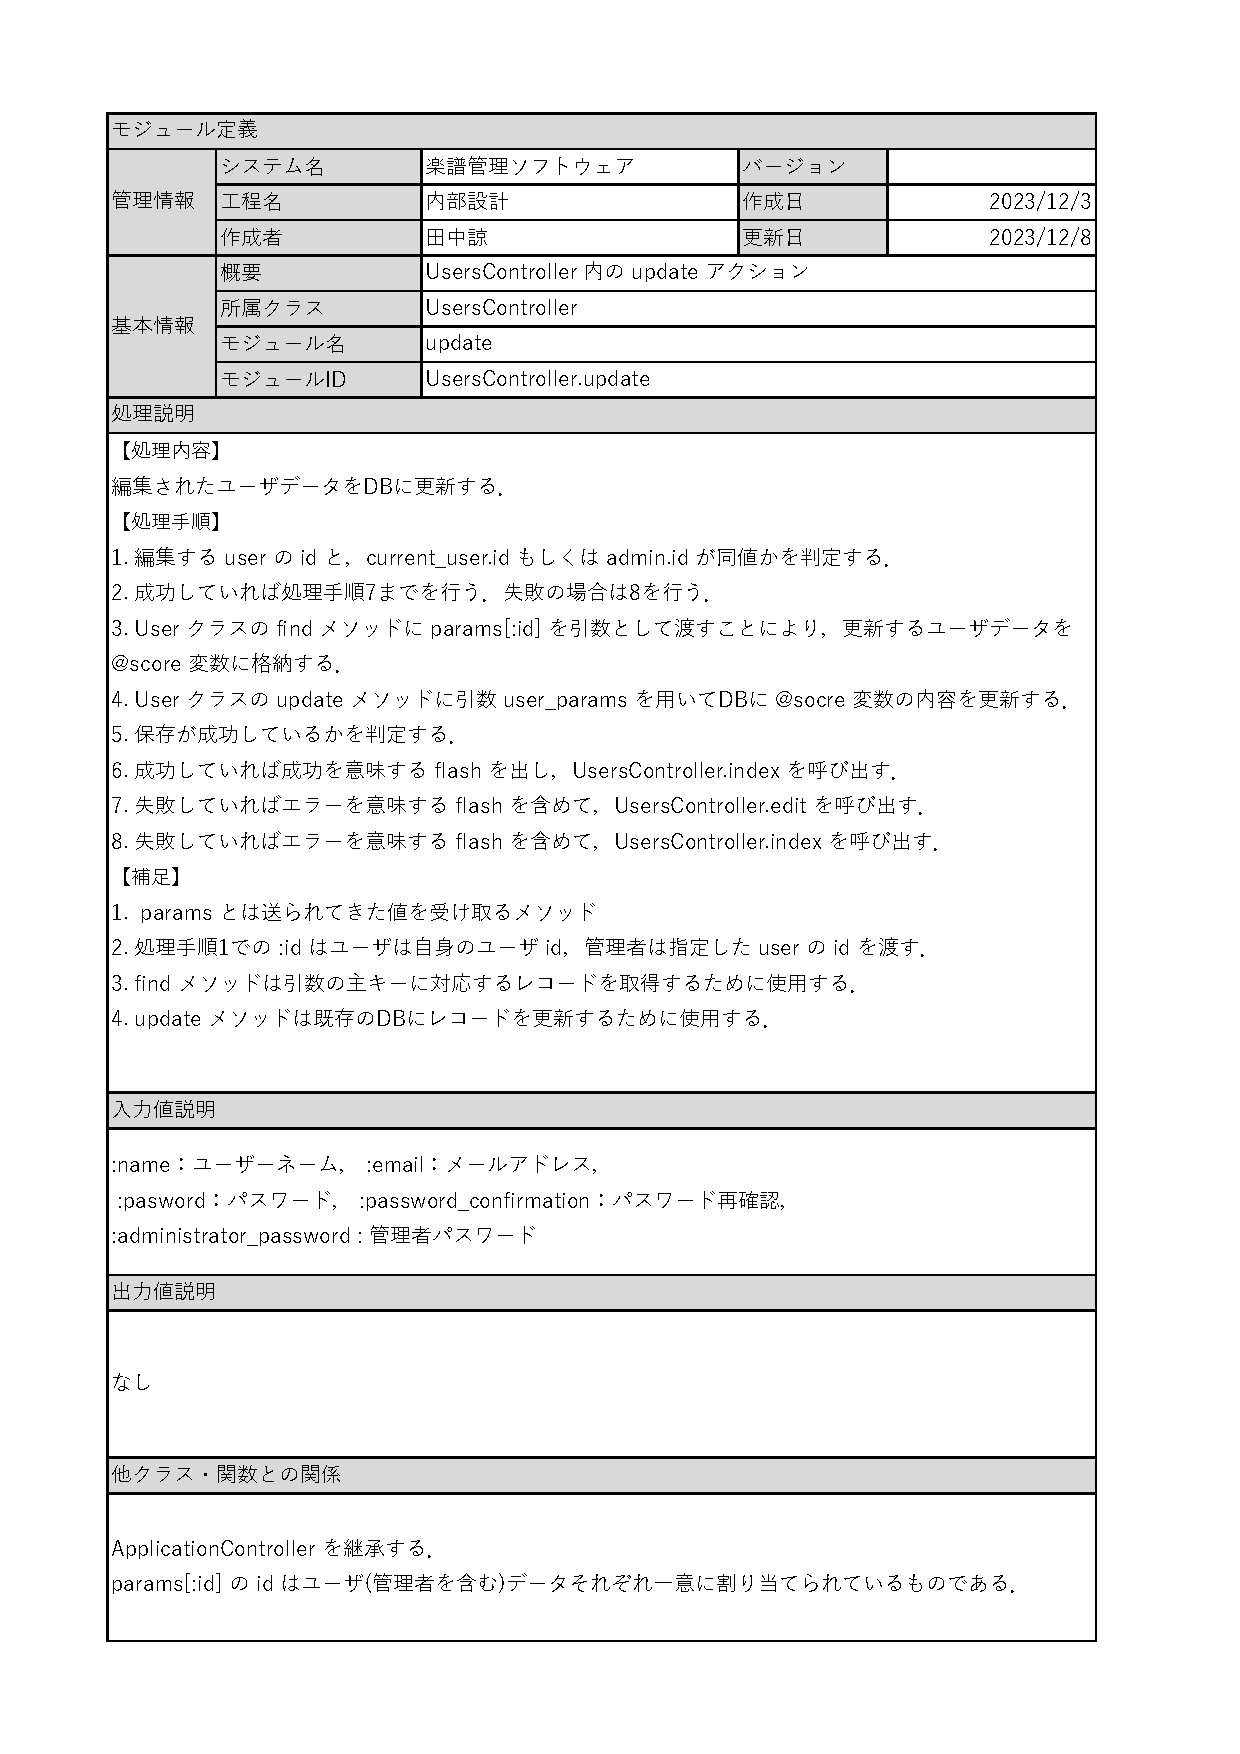
\includegraphics[scale=0.6]{img/Users/xlsx/UsersController_update.pdf}
    \vspace{-1cm}
    \caption{UsersController.update定義書}
\end{figure}
\begin{figure}
    \centering
    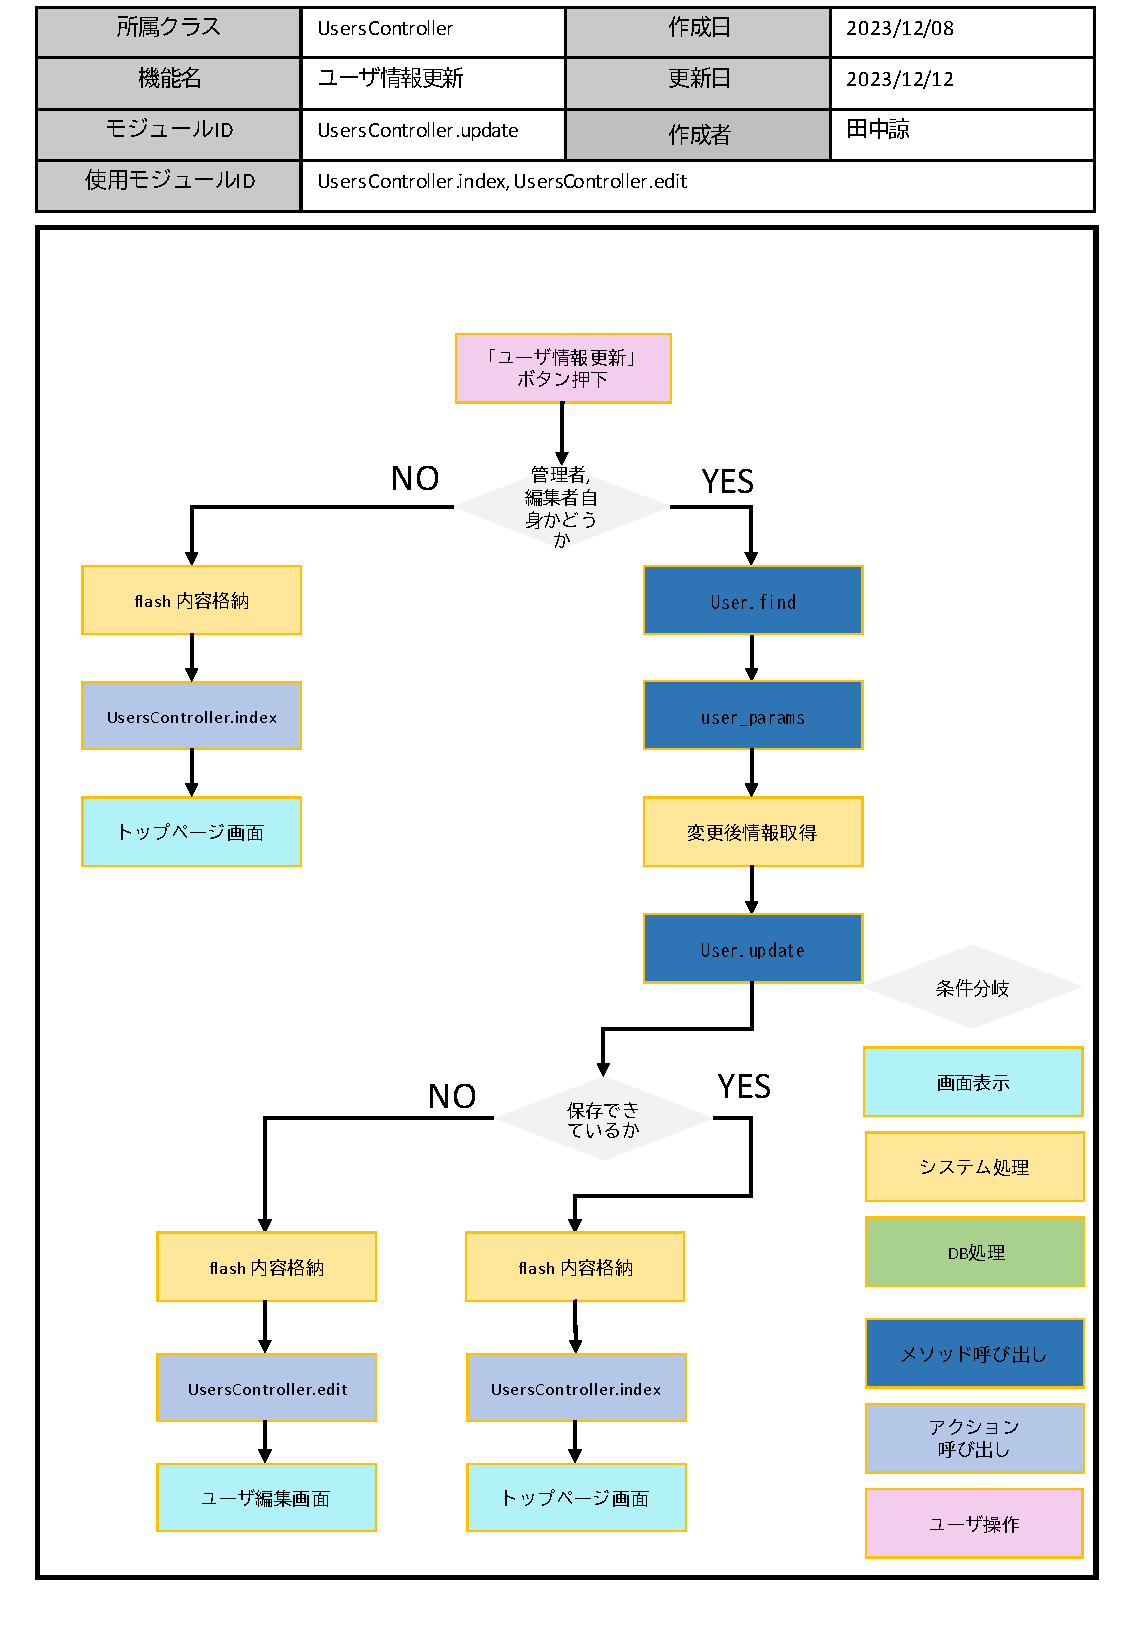
\includegraphics[scale=0.6]{img/Users/pptx/UsersController_update.pdf}
    \caption{UsersController.updateフロー図}
\end{figure}

\clearpage

%destroy
\subsection*{ScoresController クラスの destroy アクション}
既登録された楽譜データをDBから削除する機能を持つ.viewは持たない.
\begin{figure}[H]
    \centering
    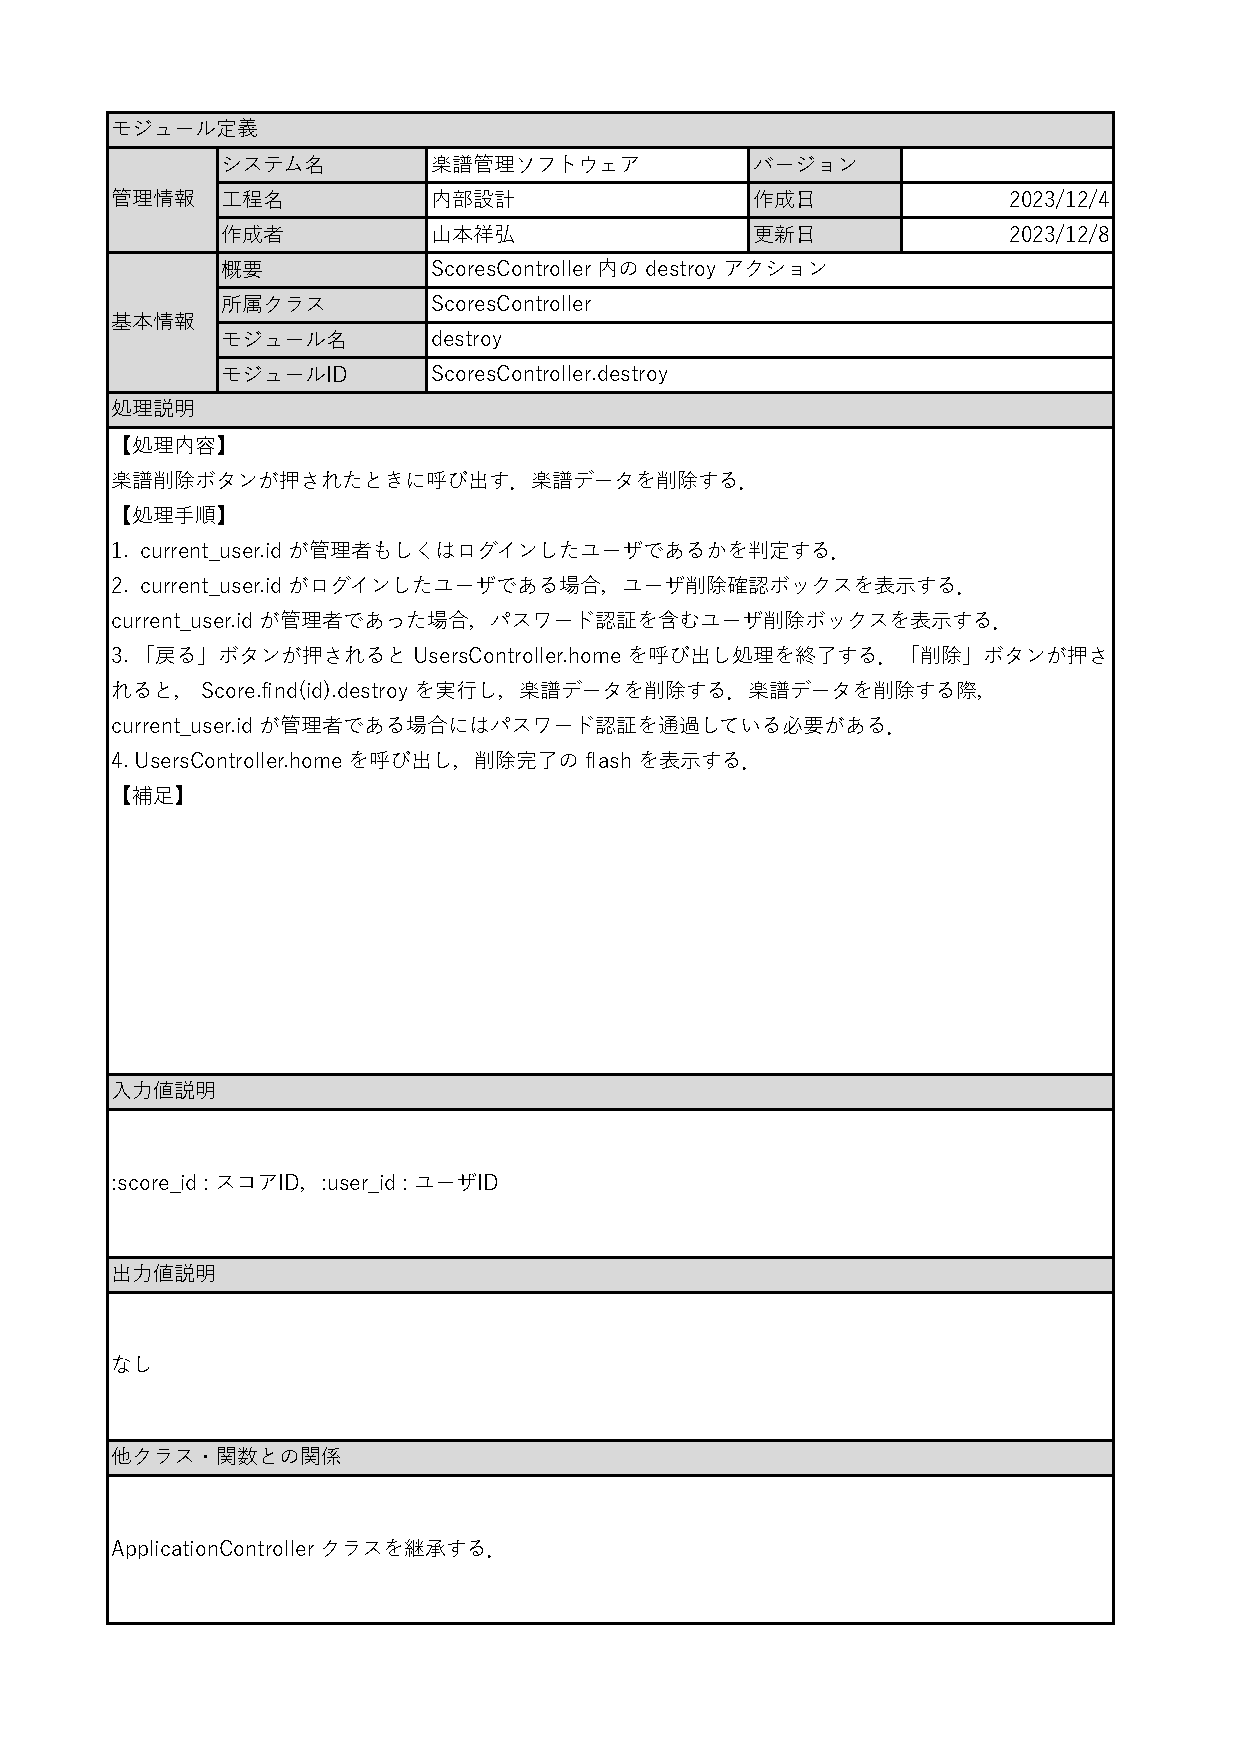
\includegraphics[scale=0.6]{img/Scores/xlsx/ScoresController_destroy.pdf}
    \vspace{-1cm}
    \caption{ScoresController.destroy定義書}
\end{figure}
\begin{figure}
    \centering
    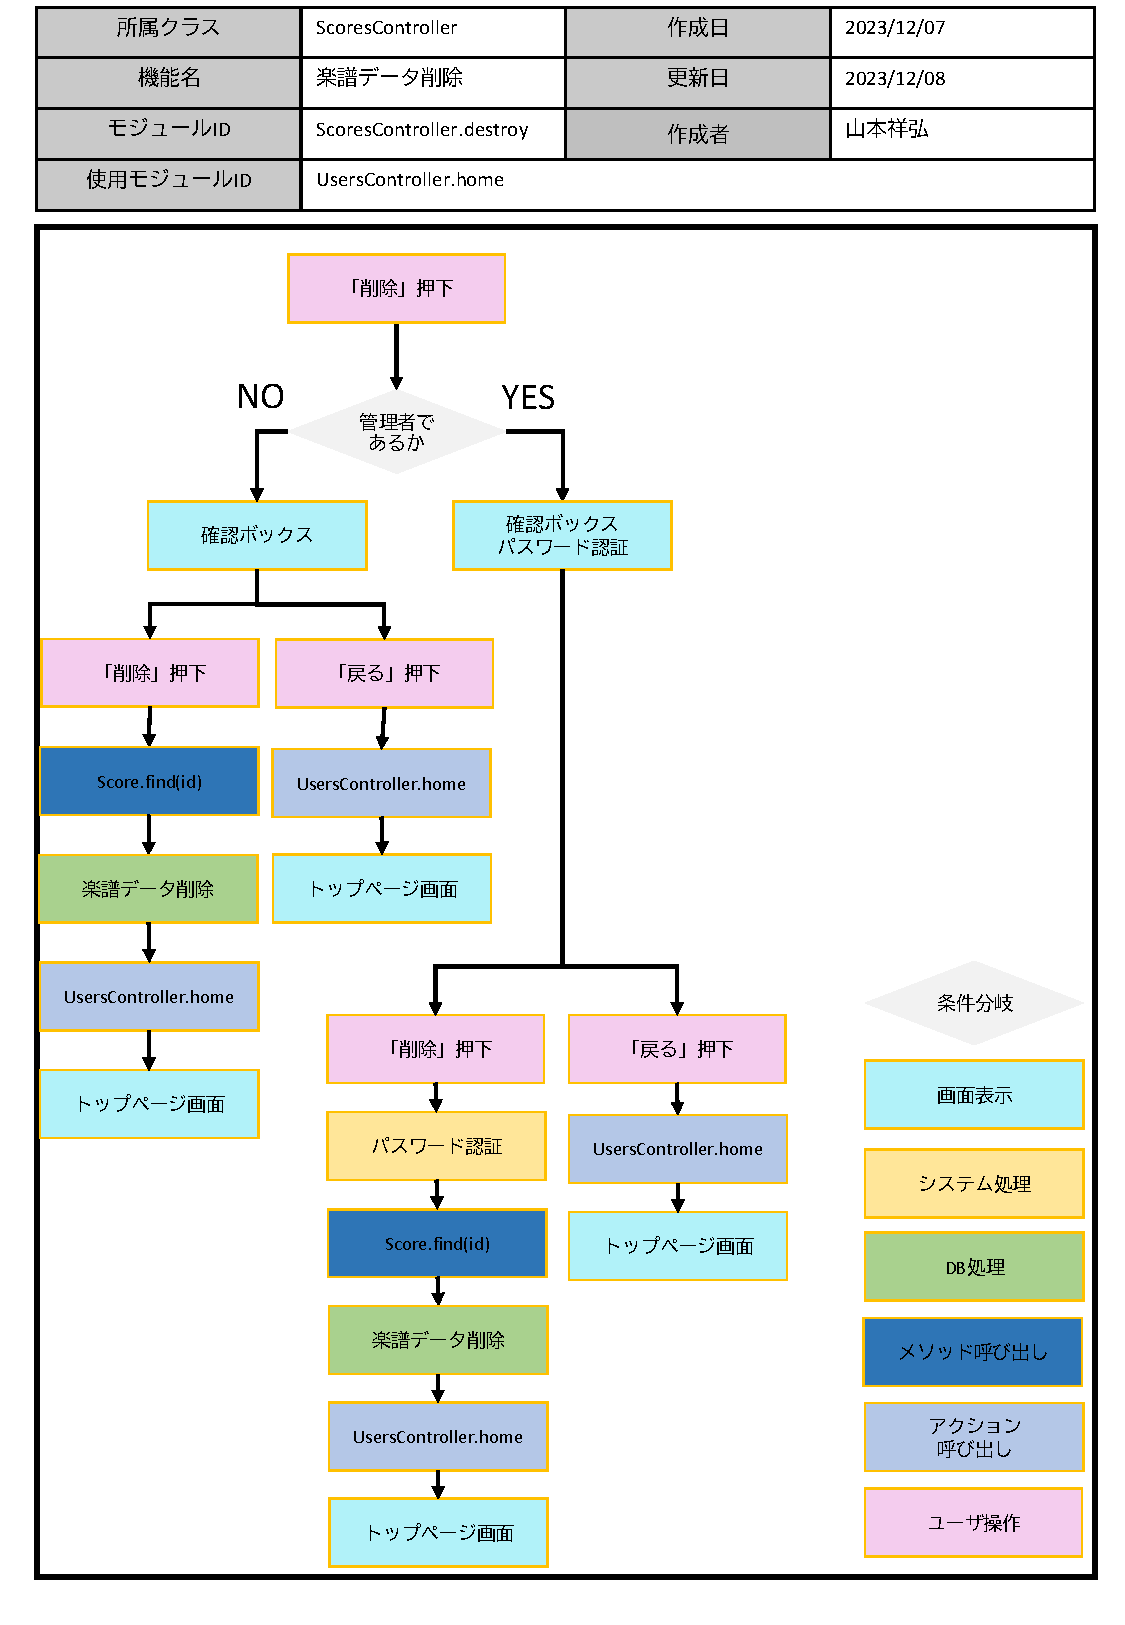
\includegraphics[scale=0.6]{img/Scores/pptx/ScoresController_destroy.pdf}
    \caption{ScoresController.destroyフロー図}
\end{figure}
\clearpage
\subsection*{UsersController クラスの destroy アクション}
既登録されたユーザをDBから削除する機能を持つ.viewは持たない.
\begin{figure}[H]
    \centering
    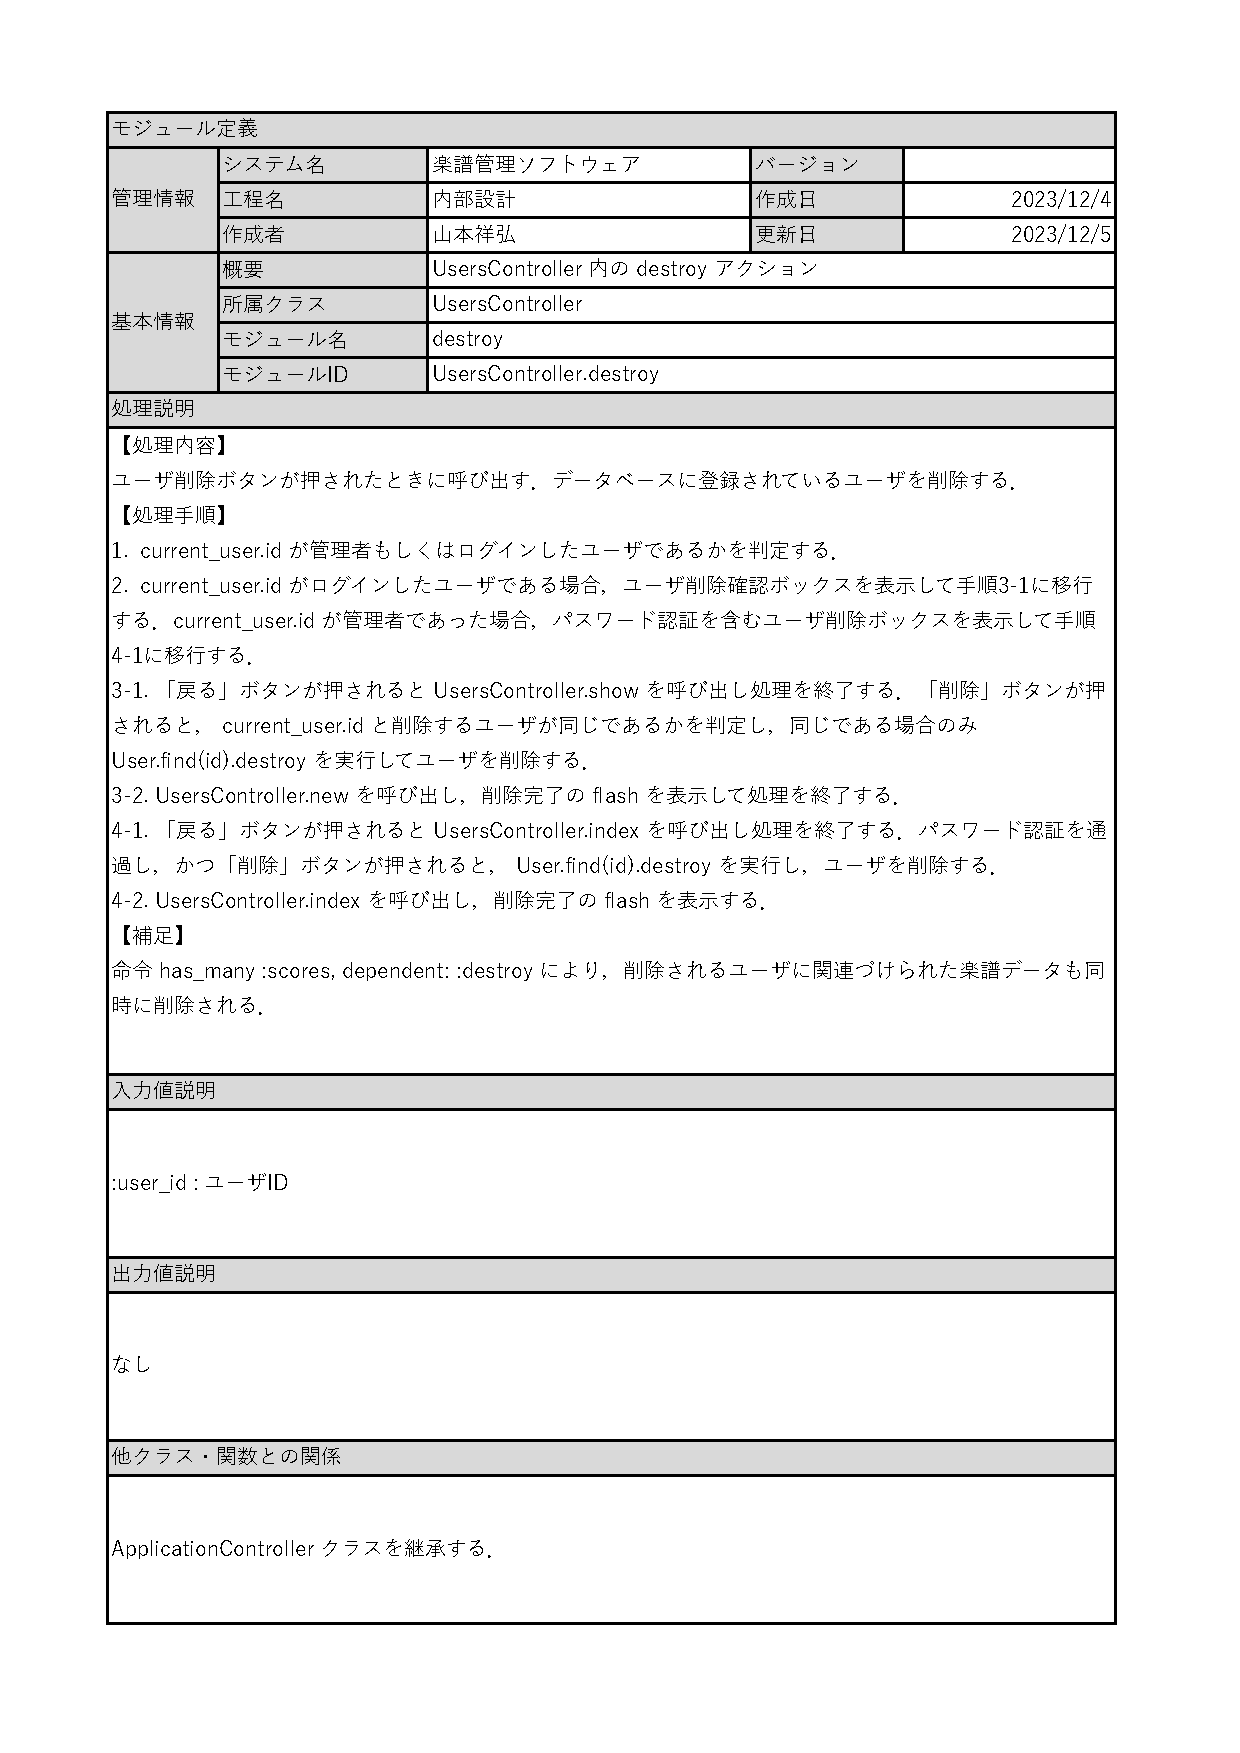
\includegraphics[scale=0.6]{img/Users/xlsx/UsersController_destroy.pdf}
    \vspace{-1cm}
    \caption{UsersController.destroy定義書}
\end{figure}
\begin{figure}
    \centering
    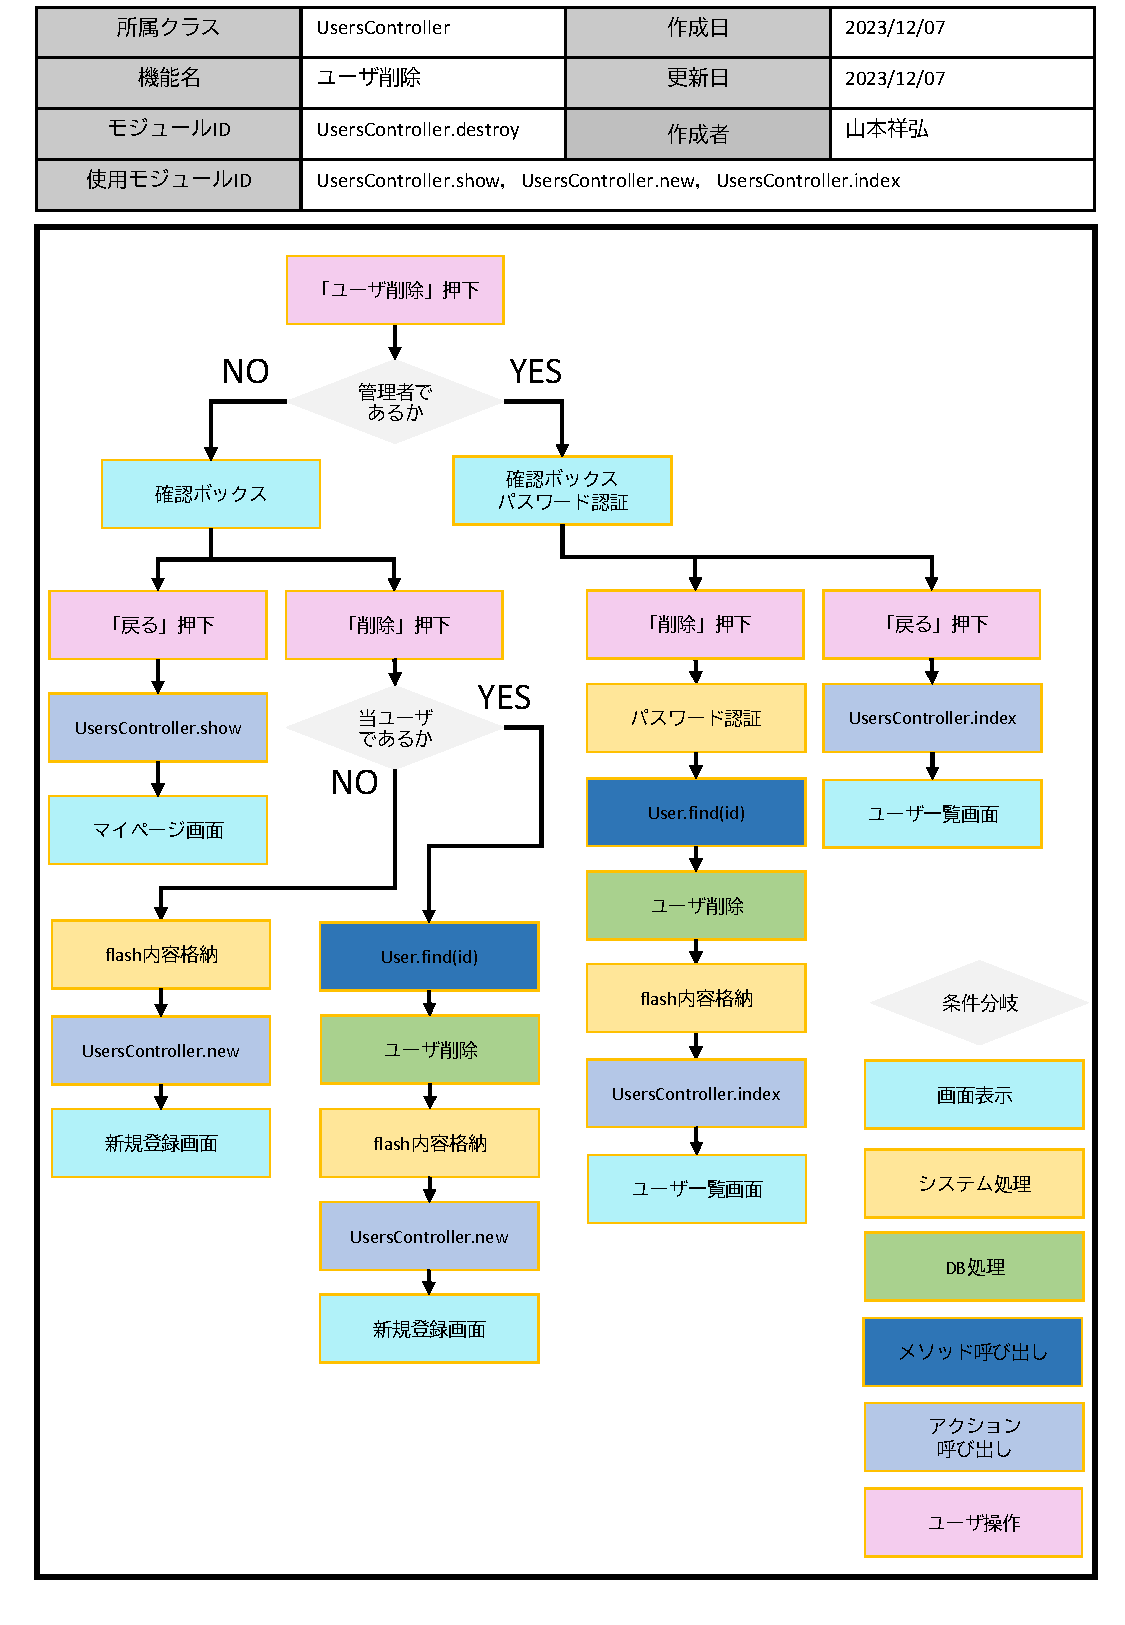
\includegraphics[scale=0.6]{img/Users/pptx/UsersController_destroy.pdf}
    \caption{UsersController.destroyフロー図}
\end{figure}

\clearpage

%session
\subsection*{SessionsController クラスの new アクション}
ログイン画面を表示する機能を持つ.対応するviewファイルを表示する.
\begin{figure}[H]
    \centering
    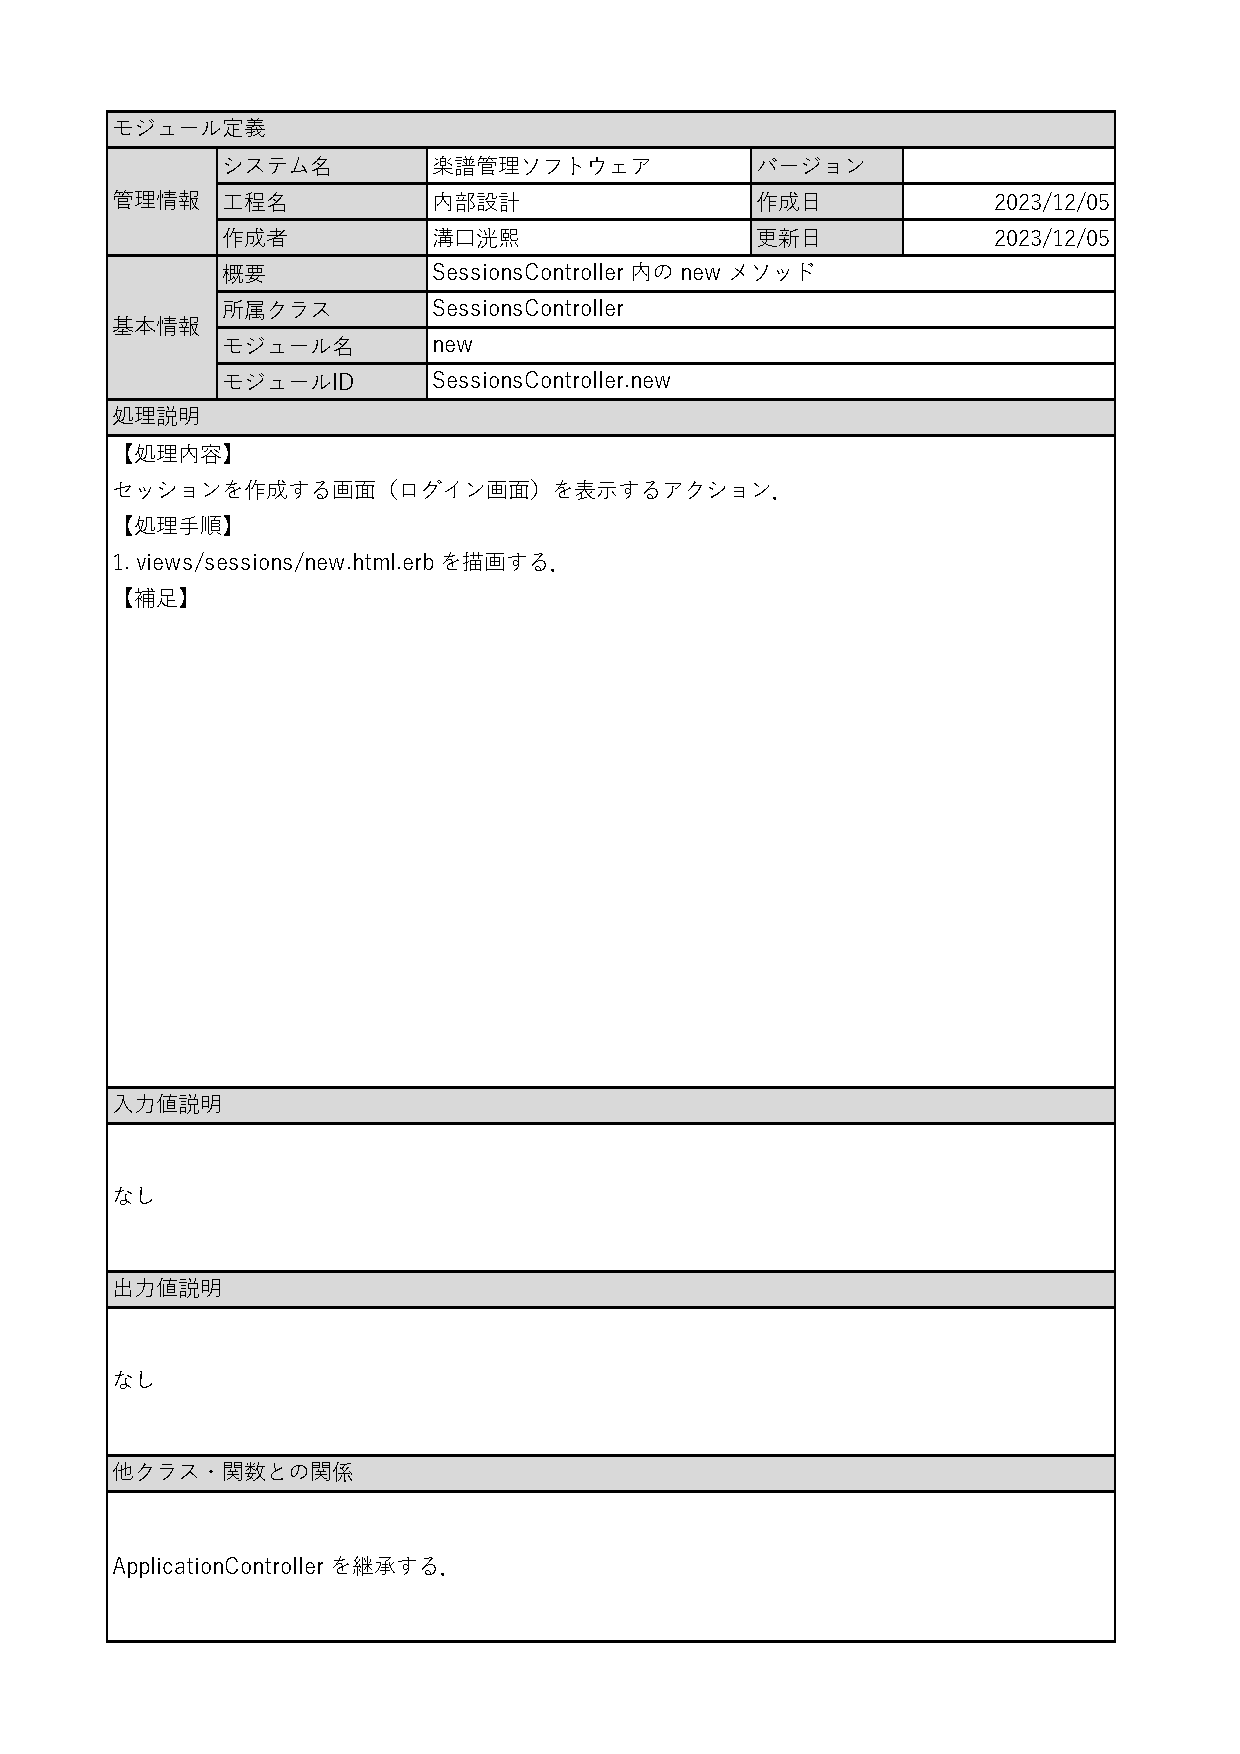
\includegraphics[scale=0.6]{img/Sessions/xlsx/SessionsController.new.pdf}
    \vspace{-1cm}
    \caption{SessionsController.new定義書}
\end{figure}
\begin{figure}
    \centering
    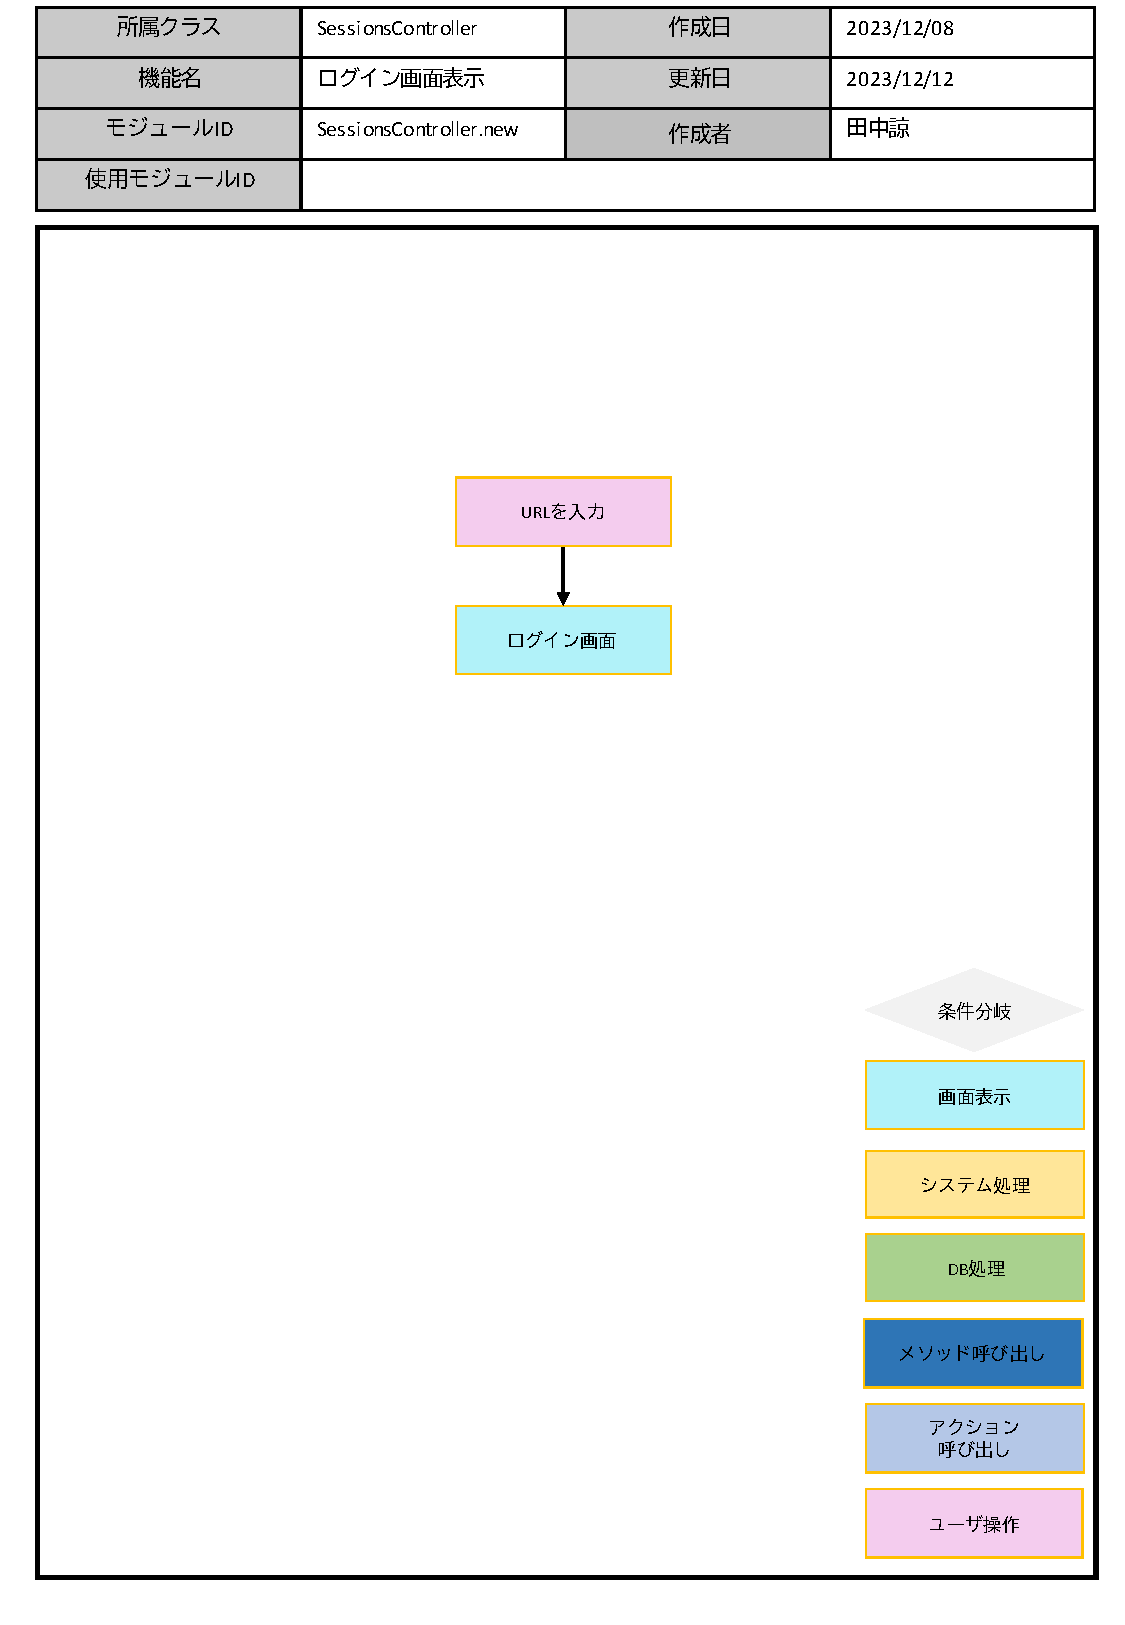
\includegraphics[scale=0.6]{img/Sessions/pptx/SessionsController_new.pdf}
    \caption{SessionsController.newフロー図}
\end{figure}
\clearpage
\subsection*{Sessionscontroller クラスの create アクション}
ログイン処理をする機能を持つ.対応するviewファイルは持たない.
\begin{figure}
    \centering
    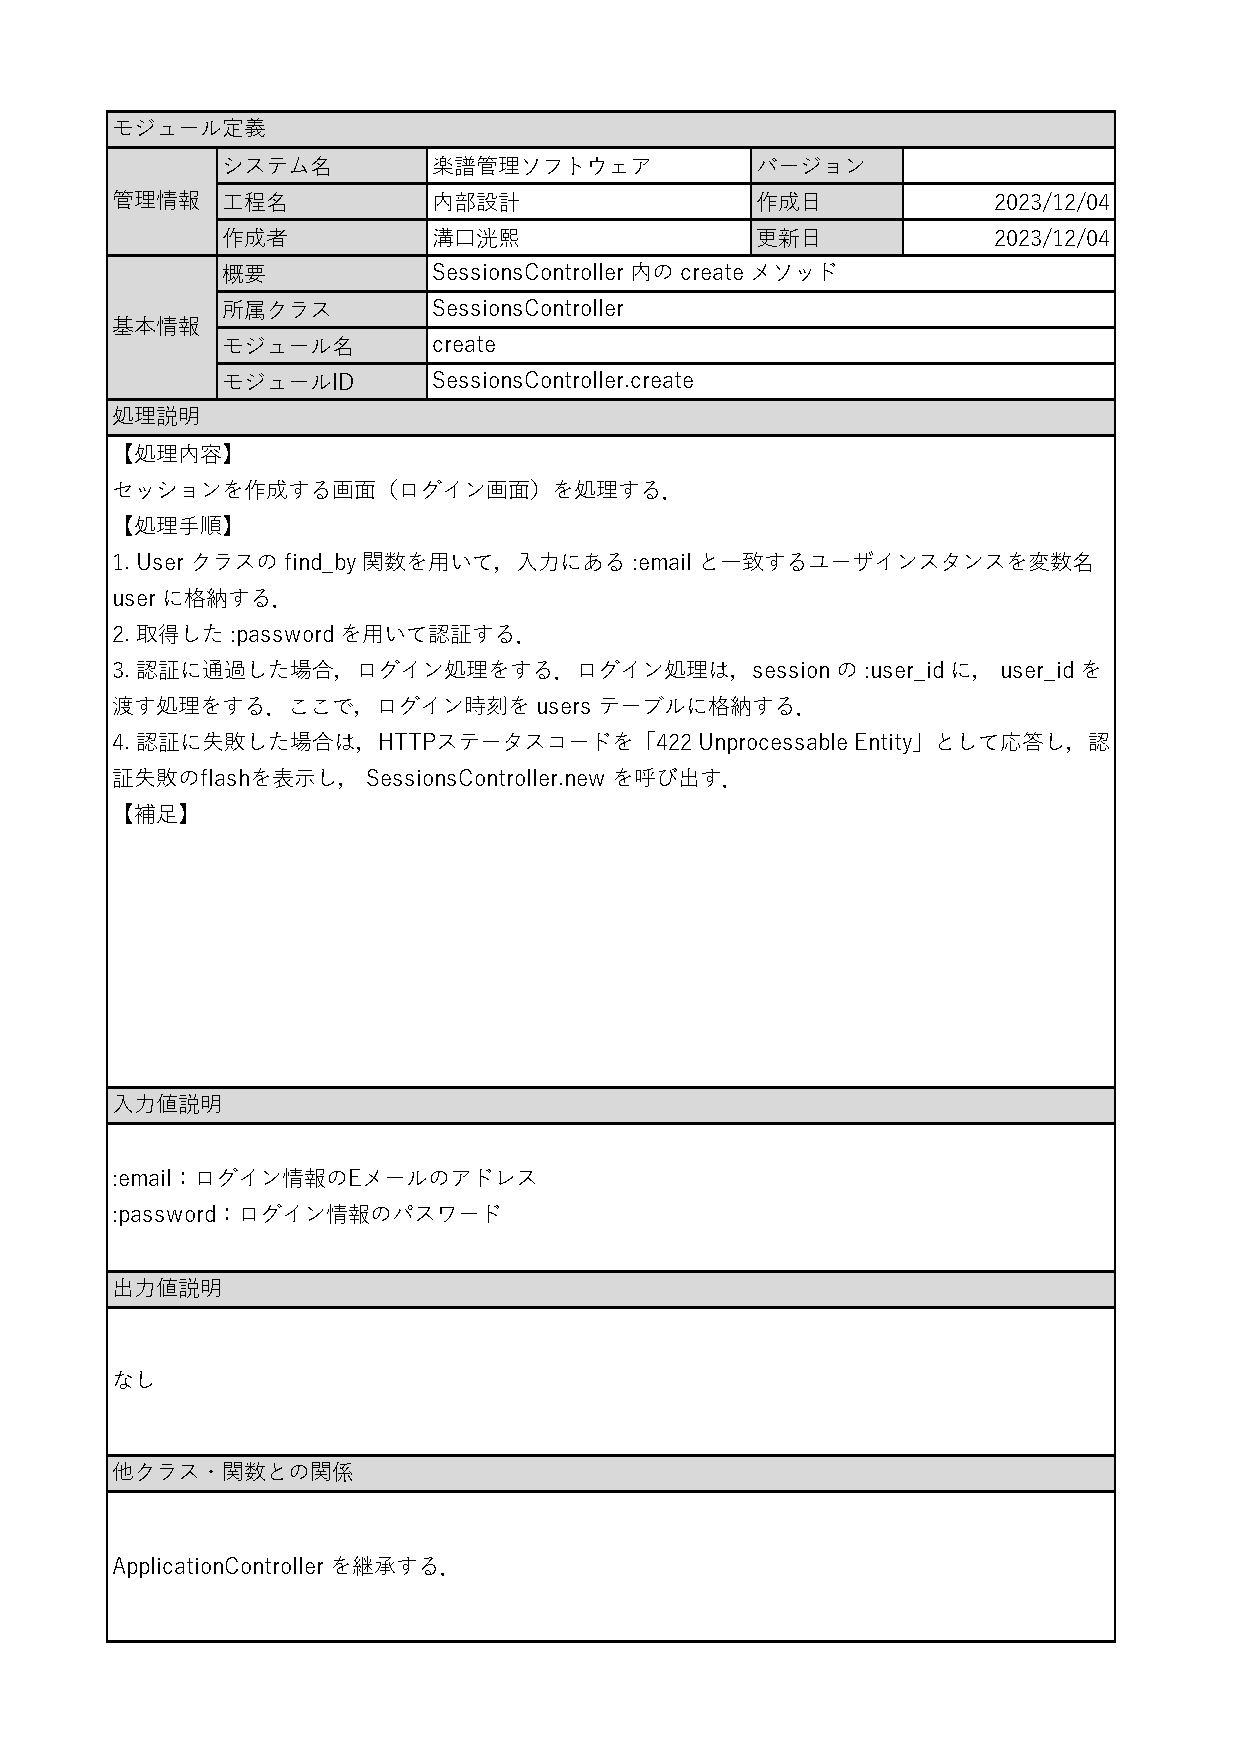
\includegraphics[scale=0.6]{img/Sessions/xlsx/SessionsController.create.pdf}
    \vspace{-1cm}
    \caption{SessionsController.create定義書}
\end{figure}
\begin{figure}
    \centering
    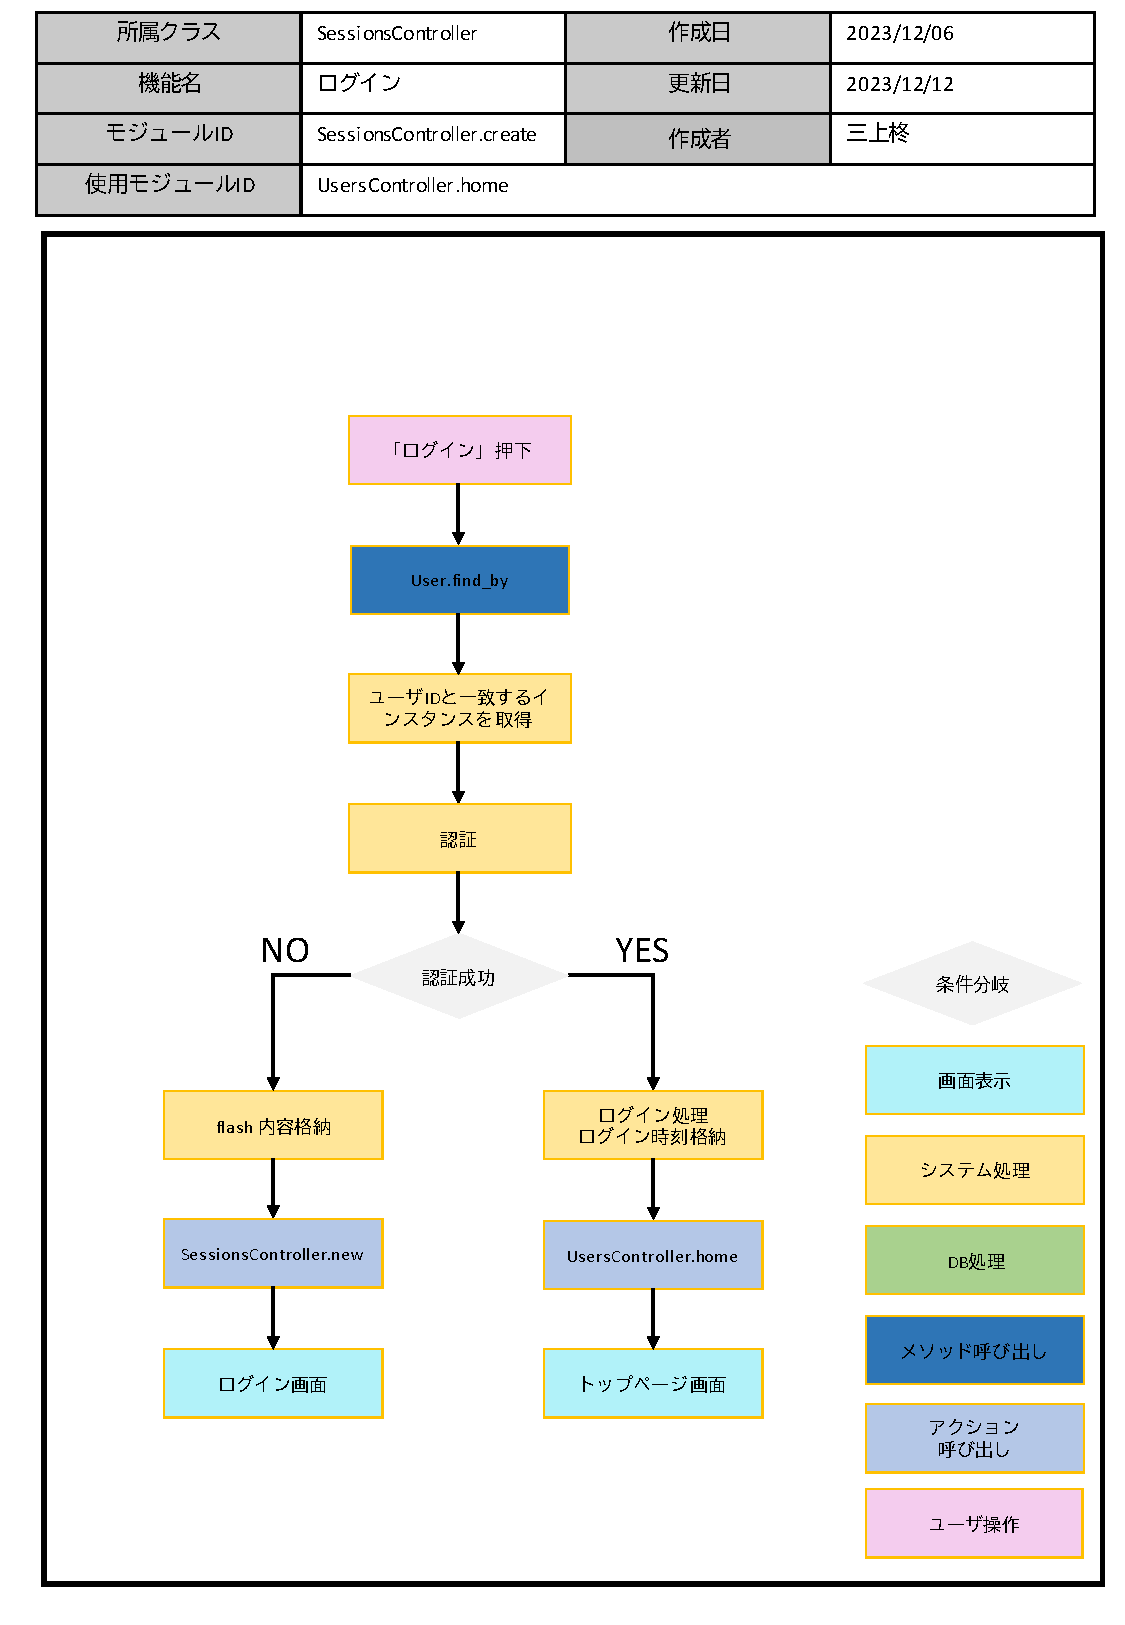
\includegraphics[scale=0.6]{img/Sessions/pptx/SessionsController_create.pdf}
    \caption{SessionsController.createフロー図}
\end{figure}
\clearpage 
\subsection*{SessionsController クラスの destroy アクション}
ユーザをログイン状態でなくす機能を持つ.対応するviewファイルは持たない.
\begin{figure}
    \centering
    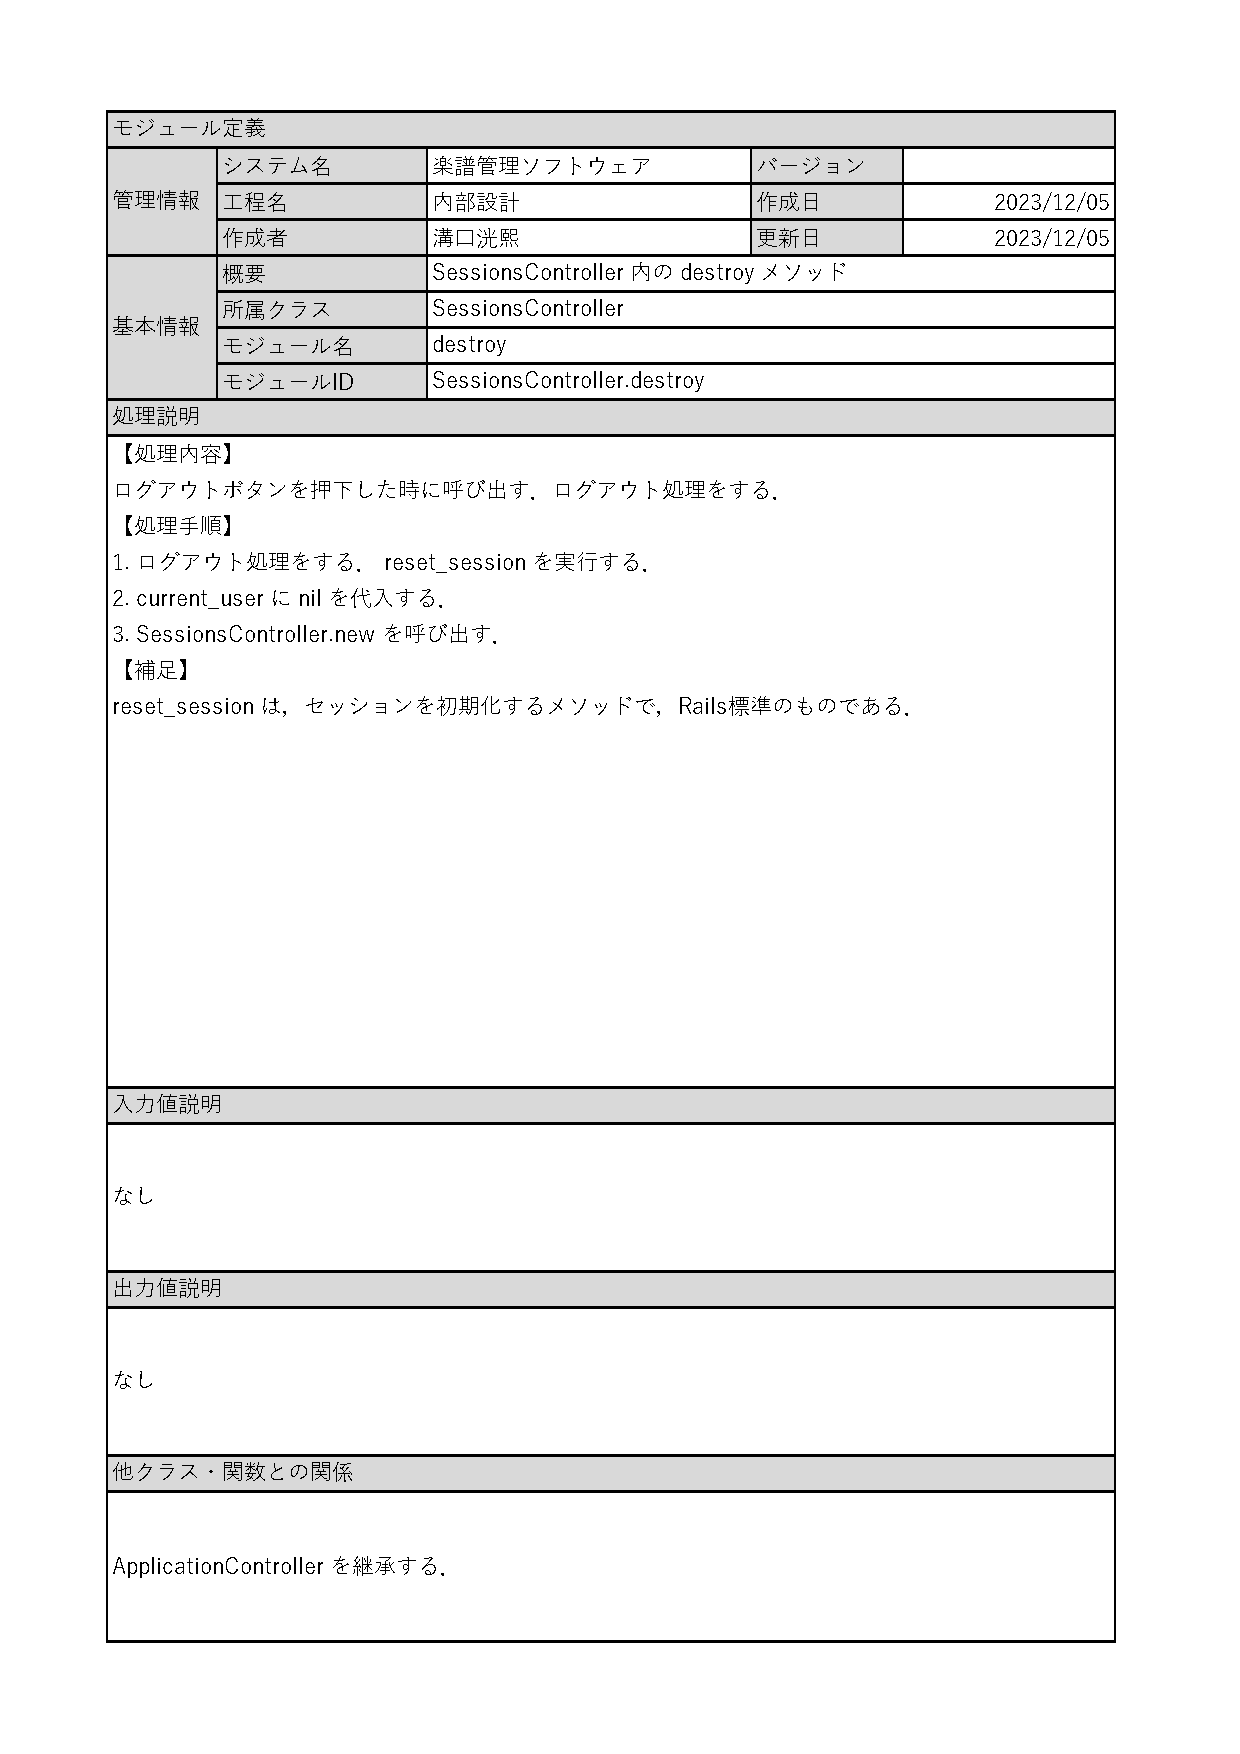
\includegraphics[scale=0.6]{img/Sessions/xlsx/SessionsController.destroy.pdf}
    \vspace{-1cm}
    \caption{SessionsController.destroy定義書}
\end{figure}
\begin{figure}
    \centering
    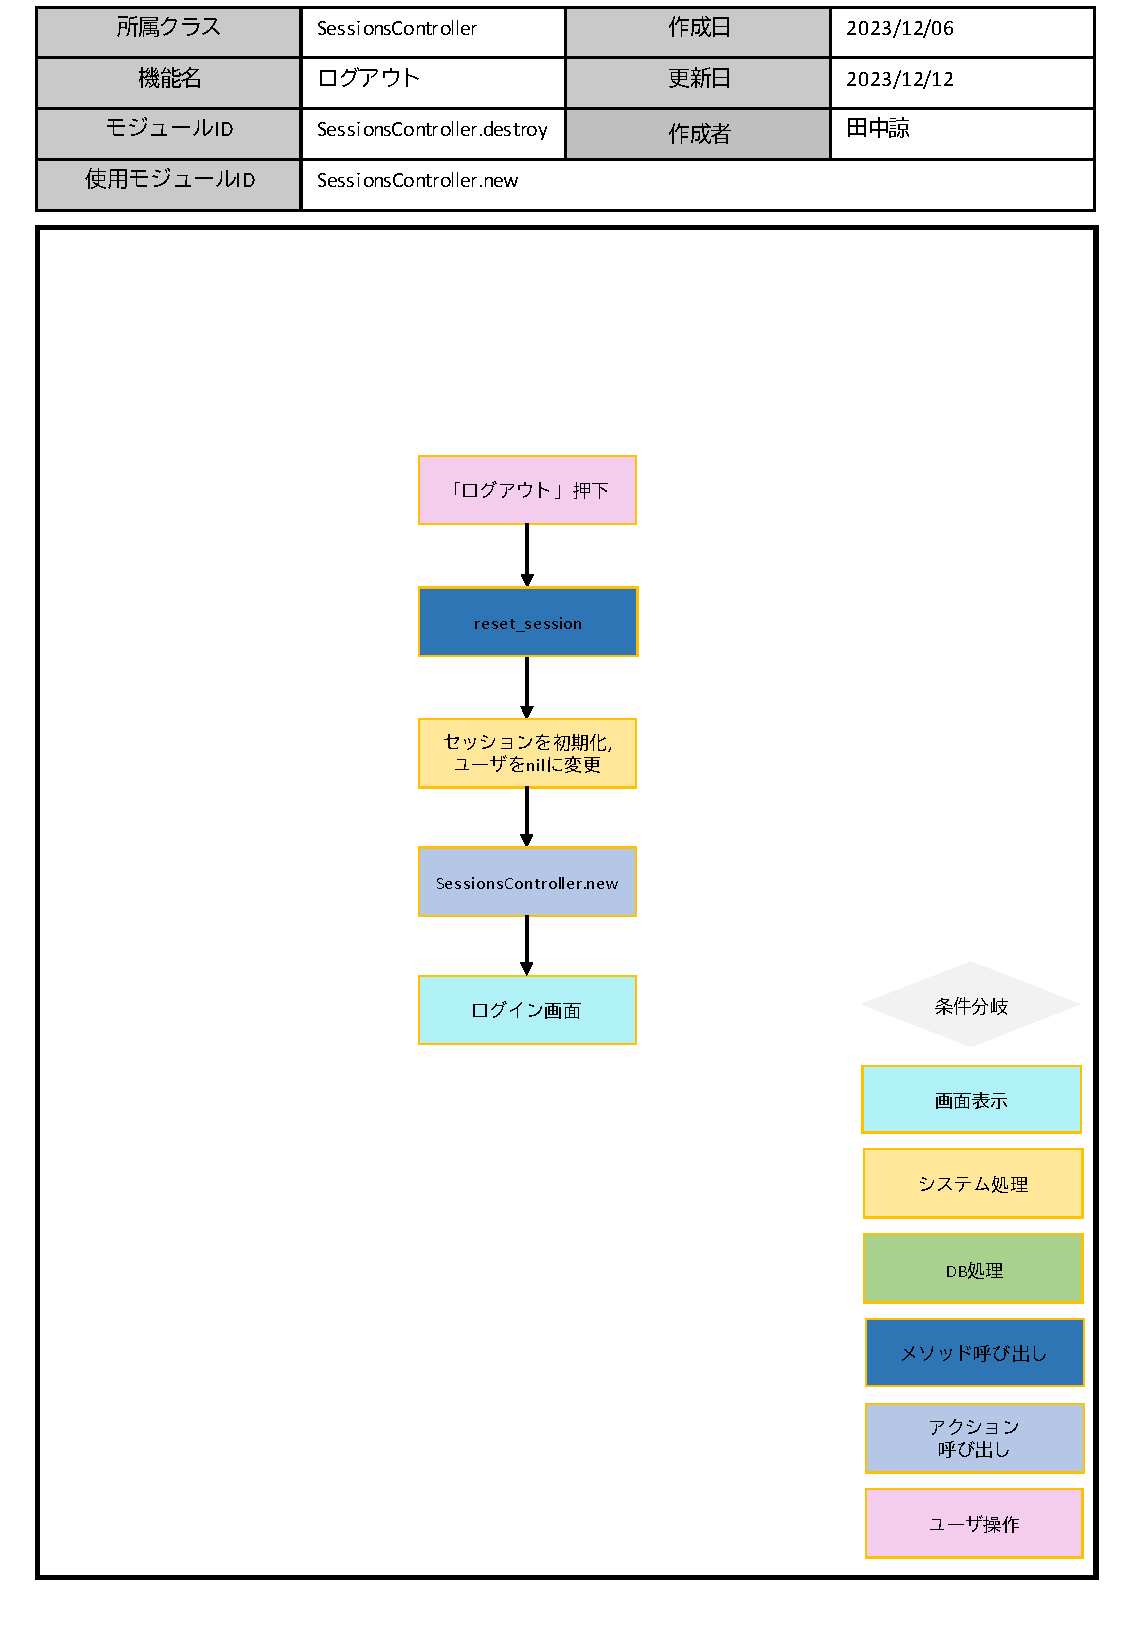
\includegraphics[scale=0.6]{img/Sessions/pptx/SessionsController_destroy.pdf}
    \caption{SessionsController.destroyフロー図}
\end{figure}
